\documentclass[12pt,a4paper,twoside]{book} % article, report or essay

\usepackage{thesis}

\begin{document}

%%%%%% Formal begining of the thesis
\pagenumbering{roman}
  
%% cover
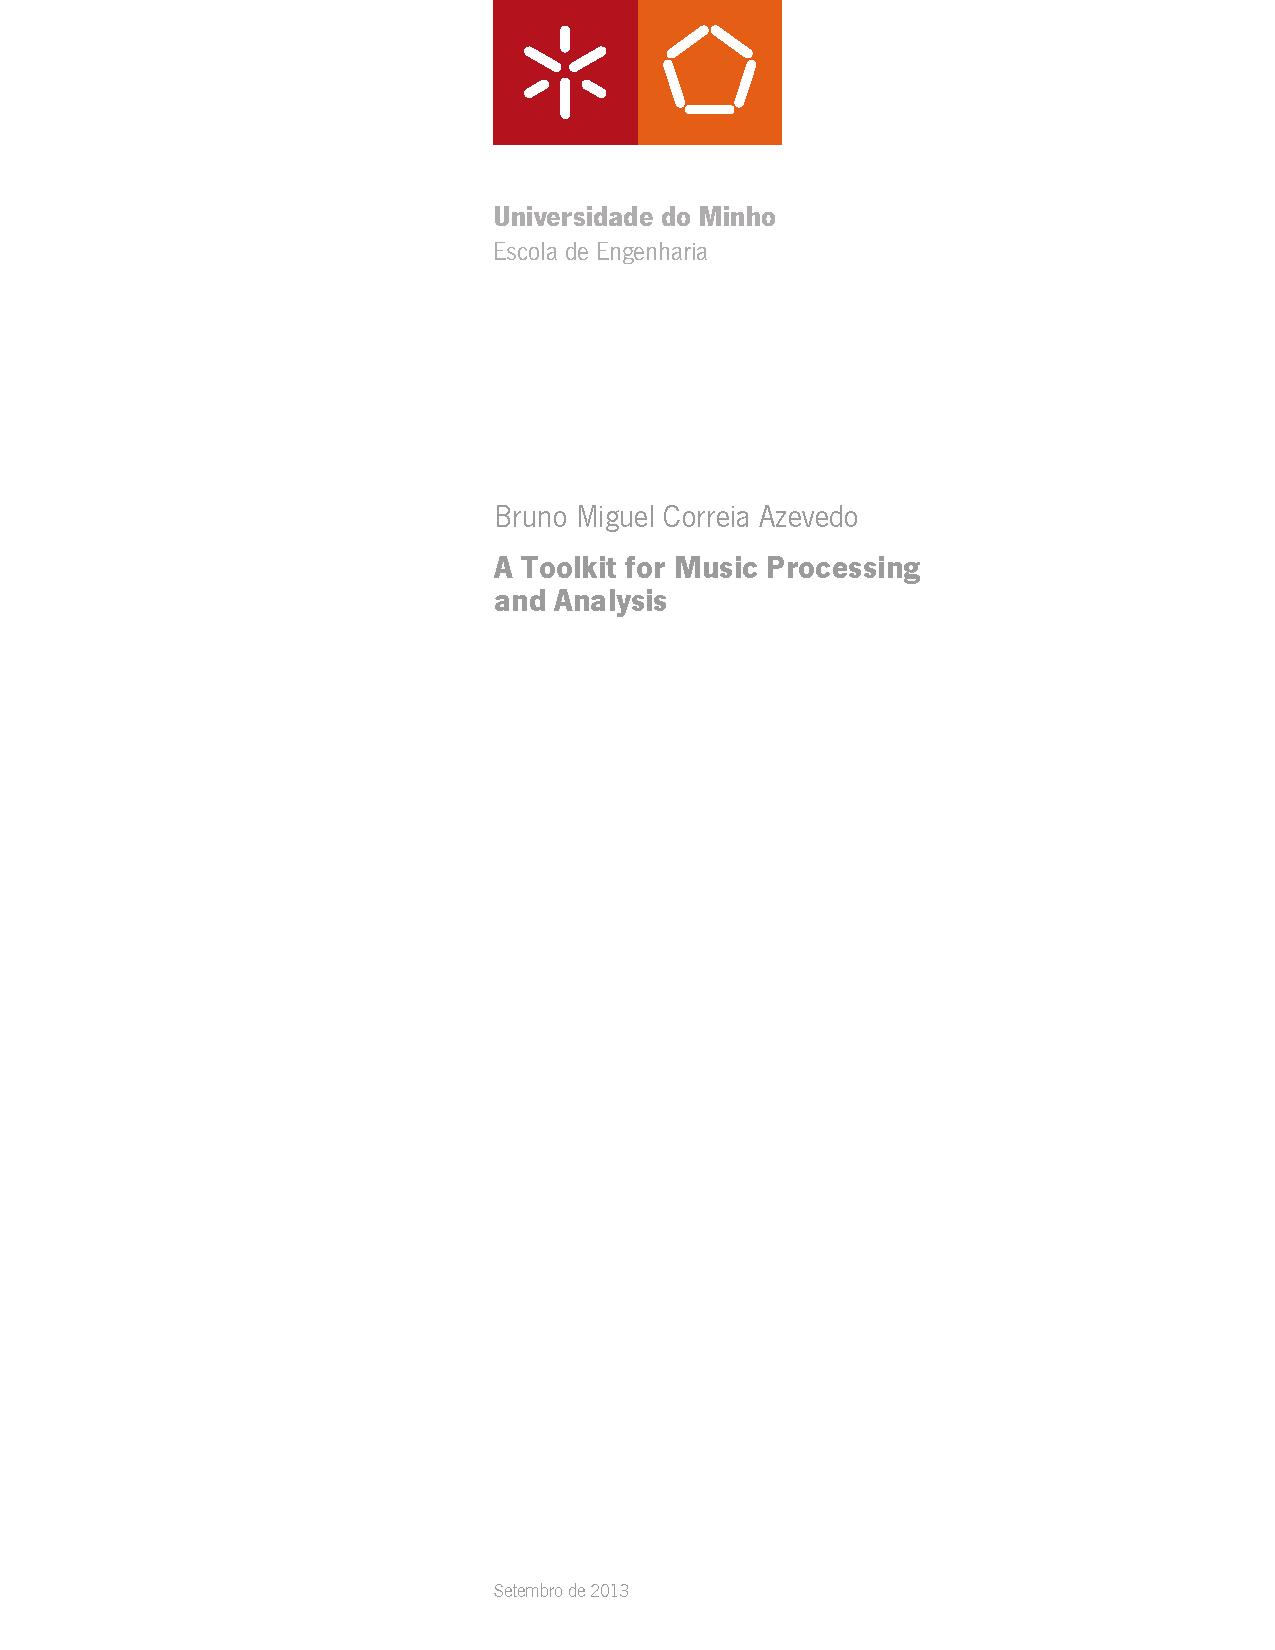
\includepdf[pages=-]{img/cover_mei} %  insert the whole pdf

\thispagestyle{plain}
%e\setcounter{page}{3}
\noindent{\LARGE\textbf{Declaração}}
\par\vspace{10mm}
\noindent{\textbf{Nome:}} Bruno Miguel Correia Azevedo
\par\vspace{3mm}
\noindent{\textbf{Endereço Electrónico:}} azevedo.252@gmail.com
\par\vspace{3mm}
\noindent{\textbf{Telefone:}} 917258220
\par\vspace{3mm}
\noindent{\textbf{Bilhete de Identidade:}} 13715148
\par\vspace{3mm}
\noindent{\textbf{Título da Dissertação:}} A Toolkit for Music Processing and Analysis
\par\vspace{3mm}
\noindent{\textbf{Orientador:}} José João Dias de Almeida
\par\vspace{3mm}
\noindent{\textbf{Ano de conclusão:}} 2013
\par\vspace{3mm}
\noindent{\textbf{Designação do Mestrado:}} Mestrado em Engenharia Informática
\par\vspace{20mm}
\noindent{É AUTORIZADA A REPRODUÇÃO INTEGRAL DESTA DISSERTAÇÃO APENAS PARA EFEITOS DE INVESTIGAÇÃO,
MEDIANTE DECLARAÇÃO ESCRITA DO INTERESSADO, QUE A TAL SE COMPROMETE.}
\par\vspace{10mm}
\begin{center}
Universidade do Minho, 1 de Setembro de 2013
\par\vspace{3mm}
Bruno Miguel Correia Azevedo
\end{center}

\newpage
\thispagestyle{plain}

%% resumo
\chapter*{Resumo}
\paragraph{}

\abc{}~\cite{abcnotation:Online} é uma notação musical simples mas poderosa que permite a produção
de partituras completas e profissionais.

Atualmente, existe uma escassez de ferramentas genéricas para processamento de notação musical,
particularmente para \abc{}.

Esta dissertação apresenta o \abcdt{}, uma linguagem de domínio
específico~\cite{kosar2010comparing,kosar2008preliminary} baseada em regras (embutida em Perl),
projetada para simplificar a criação de ferramentas para processamento de \abc{}. Inpiradas na
filosofia \unix{}, essas ferramentas pretendem ser simples e composicionais à semelhança dos filtros
\unix{}.

A partir das regras do \abcdt{} obtém-se uma ferramenta para processamento de \abc{} cujo algoritmo
principal segue a arquitetura de um compilador tradicional, dessa forma consistindo em três fases:
\textbf{1)} parsing de \abc{} (baseado no parser do \abcmtops{}~\cite{abcm2ps:Online}), \textbf{2)}
transformação semântica de \abc{} (associada a atributos \abc{}) e \textbf{3)} geração de output (um
gerador definido pelo utilizador or fornecido pelo sistema).

Um conjunto de ferramentas para processamento de \abc{} foi desenvolvido utilizando o \abcdt{}.
Cada uma delas tem uma finalidade única, desde detetar erros, a auxiliar no estudo de música e até
imitar o comportamento de algumas ferramentas \unix{}. Estas têm o objetivo de serem provas de
conceito e ainda podem ser melhoradas, no entanto demonstram quão facilmente ferramentas compactas
para processamento de \abc{} podem ser criadas.

Um teste e avaliação foram realizados a uma das ferramentas criadas (\canonabc{}) com uma partitura
\abc{} real, o \texttt{Canon de Pachelbel}.

\newpage
\thispagestyle{plain}

%% abstract
\chapter*{Abstract}
\paragraph{}

\abc{}~\cite{abcnotation:Online} is a simple, yet powerful, textual musical notation which allows to
produce professional and complete music scores.

Presently, there is a lack of music notation general processing tools, particularly for \abc{}.

This dissertation presents \abcdt{}, a rule-based
\ac{DSL}~\cite{kosar2010comparing,kosar2008preliminary} (Perl embedded), designed to simplify the
creation of \abcpt{}s. Inspired by the \unix{} philosophy, those tools intend to be simple and
compositional in a \unix{} filters' way.

From \abcdt{}'s rules an \abcpt{} whose main algorithm follows a traditional compiler architecture
is obtained, therefore consisting of three stages: \textbf{1)} \abc{} parsing (based on
\abcmtops'~\cite{abcm2ps:Online} parser), \textbf{2)} \abc{} semantic transformation (associated
with \abc{} attributes) and \textbf{3)} output generation (either a user defined or system provided
\abc{} generator).

A set of \abcpt{}s was developed using \abcdt{}. Every one of them has its single purpose, from
error detection, to aiding in music studying and even imitating some \unix{} tools behavior. They
are intended to be proof of concept and can still be improved, yet they demonstrate how easily
compact \abcpt{}s can be created.

A test and evaluation were done to one of the created \abcpt{}s (\canonabc{}) with a real \abc{}
score, \texttt{Pachelbel's Canon}.

\newpage
\thispagestyle{plain}

%% acknowledgements
\chapter*{Acknowledgments}
\paragraph{}

\begin{itemize}
  \item Thanks to my teacher José João Almeida for all the time dedicated to this dissertation, the
  supervision, the ideas and the joviality.
  \item Thanks to Jean-François Moine and Seymour Shlien for all the help given in exploring their
  tools, the prompt responses, the discussions and the good advices.
  \item Thanks to \textsc{slate'13} reviewers for their contribution to my
  paper's~\cite{Azevedo2013} improvement.
  \item Thanks to José Nuno Oliveira for the discussions and suggestions.
  \item Thanks to my family for the constant encouragement and support throughout my studies and
  also my life.
  \item Thanks to all my friends for their friendship, support and good moments.
  \item Thanks to Leandra Morais for all the moral support and encouragement when they were most
  needed.
\end{itemize}

\newpage
\thispagestyle{plain}

%% table of contents
\tableofcontents{}
\thispagestyle{plain}

%% list of figures
\listoffigures
\newpage
\thispagestyle{plain}

%% list of tables
\listoftables
\newpage
\thispagestyle{plain}

\listof{lstlisting}{List of Examples}
  
\chapter*{List of Acronyms}
\begin{acronym}[TDMA]
%A
  \acro{ASCII}[ASCII]{American Standard Code for Information Interchange}
%C
%D
  \acro{DSL}[DSL]{domain-specific language}
%E
%H
%I
  \acro{IR}[IR]{internal representation}
%J
%L
%M
%O
%R
%S
  \acro{OS}[OS]{Operating System}
%U
%V
%W
%Y
\end{acronym}

\newpage
\thispagestyle{plain}
\cleardoublepage
  
%%%%%% Content
\pagenumbering{arabic}
  \acresetall
  
  %% chapters
  % Why am I doing it? What do I hope to discover?
  \chapter{Introduction}
  \label{chap:intro}
  \section{Context and Motivation}
\subsection*{Textual Musical Notation}

All music needs to be written before read, comprehended or performed by any musician. To make it
possible, a notation system has been developed that provides musicians with the information
necessary to reproduce it as the composer wanted.

The notation consists in any system that represents audible music through written symbols. The use
of symbolic and abstract formats improves music reasoning, as it gives the composer a greater
freedom to express his music and provides easier readability to the performer.

As computers were introduced to the world of music, a variety of file formats and textual notations
emerged in order to describe music, such as, \abc{}~\cite{abcnotation:Online},
LilyPond~\cite{lilypond:Online} or MusicXML~\cite{musicxml:Online}.

\abc{} is used as the base notation throughout this dissertation.

\subsection*{\unix{} Metaphor}

In the 1970s the \ac{OS} \unix{} was born and with it a new philosophy\cite{raymond2004art} based on
the principle of creating simple, yet capable and efficient programs, which tackle only one problem
at a time.

The system's interface is the command line, thus making the work method very powerful and flexible
as it enables the automatic execution of commands. Moreover, commands handle text streams as a
universal type, allowing programs to be chained.

% There are some \unix{} commands whose behavior can be adapted:
% \begin{description}
%   \item[grep:]
%     Prints the lines of a file matching a pattern;\\
%     It could print melodic sequences matching a pattern. The pattern could be a sequence of melodic
%     intervals or rhythms;
%   \item[diff:]
%     Compares files line by line;\\
%     It could compare files voice by voice;
%   \item[\ldots]
% \end{description}


In order to facilitate the development of new \unix{} commands, \unix{} creators built a new
language (C).

\begin{quotation}
  \small\textit{\unix{} is simple. It just takes a genius to understand its simplicity.}
  \begin{flushright}
    Dennis Ritchie
  \end{flushright}
\end{quotation}

When moving to the music world, the goal is to build simple music commands, using a universal music
stream type - \abc{} -, creating a development language for conceiving music commands and exercising
command compositionality.

%% CLAIM %%
Each command - an \abcpt{} - assists in the solving of music related problems. For instance,
questions like \textit{"How many times does that happen in Beethoven's sonatas?"}, or \textit{"I
wish I could extract these parts from this score and transpose them up a major second"} could be
easily answered.

%% CLAIM %%
As \unix{}, with its universal interface - the text stream -, an \abcpt{} uses \abc{} as its
universal interface. Being text as well, an \abcpt{} can be chained with others.

%% CLAIM %%
There are many \unix{} commands whose functionality can be mapped to an \abcpt{}. This is true mainly
because of the textual nature of their input. Here are some \unix{} commands that could be mapped to
\abcpt{}s: musical cat, paste, wc, grep, diff, cut, join, sed, ...

\subsection*{\abc{} toolkit}

%% CLAIM %%
Presently, there is a lack of music notation general processing tools, particularly for \abc{}. So
the main goal is to build an \abc{} \ac{OS}, i.e. a system that provides a set of \abcpt{}s that
deal with real \abc{} and aid in musical tasks like analysis, composition, studying, ...

\subsection*{\abcdt{}}

%% CLAIM %%
In order to easily build simple and compositional (in a \unix{} filters' meaning) \abcpt{}s, a
system capable of precisely specifying how an \abc{} score should be processed is needed. The same
necessity appeared to \unix{}'s developers while developing it, from which the C language was built.
Therefore, a rule-based \ac{DSL}~\cite{kosar2010comparing,kosar2008preliminary} was created - \abcdt{}.

\subsection*{Application Areas}

In order to better understand the benefits of the toolkit being proposed, some real life activities
where those tools can help make a difference are described next:

\begin{description}
  \item[Musical Wikis] \hfill \\
    Wikis that deal with the edition of musical scores. E.g.: Wiki::Score.
  \item[Cultural and cooperative volunteering] \hfill \\
    In environments like Wikis where the edition of documents happens concurrently in cooperation
    with many elements. E.g.: Wiki::Score.
  \item[Score transcription] \hfill \\
    Often errors occur while manually transcribing a score and those errors are not easily detected.
  \item[Music learning] \hfill \\
    Custom tools may be created with the purpose of supporting tasks such as studying and
    rehearsing.
  \item[Musical analysis and composition] \hfill \\
    E.g.: Through the detection of certain patterns in specific musical style it is possible to
    assess if a composition uses any feature of that style;\\
    E.g.: Automatic classification of scores;\\
    E.g.: Verification of a score's authorship. In the same way that it is possible to assess the
    probability of an author having written a certain text through the type of vocabulary used.\\
    E.g.: Generation of scores that follow strict structural rules, such as the canon or the fugue.
\end{description}

The next section presents the work developed in the context of this dissertation, enumerating the
design goals that guided the project's development. Section \ref{sec:case_studies} introduces the
case studies which served as motivation to this work and Section \ref{sec:document_structure}
presents the structure of the document, including a summary of each chapter.


\section{Project Overview}
The main goal for this project is to have a set of \abcpt{}s. Each tool deals with a specific
problem and tries to solve it in a simple and efficient way. In order to simplify the creation of an
\abcpt{}, a rule-based \ac{DSL} - \abcdt{} - was designed. From \abcdt{}'s rules an \abcpt{} is
obtained whose main algorithm follows a traditional compiler architecture.

\subsection*{Design Goals}

A set of design goals was defined to guide the project's implementation.

\subsubsection*{Toolkit}
% Problems associated with the processing of textual musical notation:
% 
% \begin{description}
%   \item \textbf{Automatic validation of the notation and error detection} \hfill\\
%     When writing \abc{}, since it is \ac{ASCII} based, it is relatively easy to write errors on the score.
%     One of the features that is required for this toolkit is for it to be able to detect those
%     errors thus validating the notation in terms of syntax, lexicon, among others that are listed
%     below:
%     \begin{itemize}
%       \item \textbf{syntax}\\
%         e.g.: beats per measure, different key definitions in voices;
%       \item \textbf{lexicon}\\
%         e.g.: inappropriate use of symbols;
%       \item \textbf{misalignment}\\
%         e.g.: voice disparity due to transcription errors;
%       \item \textbf{suspicious use of musical symbols}\\
%         e.g.: use of chords out of context in a certain musical style;
%         e.g.: use of notes out of vocal range;
%     \end{itemize}
%   \item \textbf{Error fixing} \hfill\\
%     Since it can detect erros it's only natural that they can be fixed, either by automatically
%     setting the appropriate fix or by suggesting one to the user. Typically the errors fixed will be
%     of syntactic or lexical nature.
%     \begin{itemize}
%       \item \textbf{syntactic}\\
%         e.g.: when there are many consecutive rests, then a suggestion is made to join them by
%         measure;
%         e.g.: when the key is changed in only one voice, then that change is reproduced in all %         voices;
%       \item \textbf{lexical}\\
%         e.g.: when there's an orthographic or a capitalization error in reserved words, then it is
%         automatically fixed;
%     \end{itemize}
% \end{description}

Each \abcpt{} should:

\begin{itemize}
  \item \textbf{Deal with real \abc{} music} \hfill\\
    Each tool should be able to deal with more than just a sequence of notes. Musical elements other
    than notes and rests, like lyrics or accompaniment chords, are parsed and can be processed.
    Also, unexpected elements shouldn't break the tool's process.
  \item \textbf{Follow the \unix{} philosophy} \hfill\\
    Each tool tackles a single problem and can be composed with others to solve more complex
    problems.
  \item \textbf{Be open-source} \hfill\\
    The source code will be available to the general public therefore it will follow community
    practices and will be installable and usable as a third-party tool. The existence of an
    open-source community allows the exchange of information and ideas between developers and users.
    Interesting things can come out of a discussion in this mean, like new features or a solution to
    a certain problem.
\end{itemize}

\subsubsection*{ABC::DT}

\abcdt{} is a rule-based \ac{DSL} which aims to help the creation of \abcpt{}s in a simple and
compact way. Therefore, in order to achieve that simpleness it must have the following features:

\begin{itemize}
  \item Generate simple tools through a compact specification
  \item \abc{} oriented
  \item Associate transformations with specific \abc{} elements, allowing a surgical processing
  \item Rich embedding mechanisms (using Perl for specific \abc{} transformations)
  \item Apply the identity function to not specified elements (default transformation)
  \item Processing guided by the music's internal structure
  \item Transform and manipulate the internal structure as it best suits the task at hand for a more
  efficient processing
\end{itemize}

\subsubsection*{Musical Information Representation}

A score's \ac{IR} must:

\begin{itemize}
  \item \textbf{Keep the original order of the score elements} \hfill\\
    This is an obvious goal since almost every task needs to know the exact order of a score to
    produce anything useful.
  \item \textbf{Hold sufficient musical information to rebuild the score as it was} \hfill\\
    This way a score can easily be outputted as it was originally.
  \item \textbf{Have different views of its structure} \hfill\\
    In order to have a thorough and efficient processing, the structure may be reorganized into one
    oriented to the part (for melodic tasks), to the time (for harmonic tasks) or to the source (for
    general tasks, mainly to be able to reconstruct the original \abc{}).
  \item \textbf{Facilitate the application of scripting} \hfill\\
    This means the \ac{IR} can be serialized into a structure that is easily evaluated by a language
    like Perl.
\end{itemize}

\subsubsection*{Musical Corpora}

In order to do statistical analysis there must be:

\begin{itemize}
  \item \textbf{Musical corpus comprised of musical scores} \hfill\\
    This corpus will be used as a source of data for the analysis as well as testing material.
  \item \textbf{Build tools for statistical calculation} \hfill\\
    Each tool will output some statistical information.
\end{itemize}

\subsubsection*{Musical Information Visualization}

There are always different forms for displaying musical information to a user. Be it a graph, a
drawing, some sort of symbol, the actual score or even simple text, the output must always transmit
knowledge to the user so that a conclusion can be taken from it. Thus a tool's output must:

\begin{itemize}
  \item \textbf{Have an appropriate format (textual, graphical, other)} \hfill\\
    So that the user can make the most out of the tool's results.
  \item \textbf{Be easy to comprehend} \hfill\\
    The results cannot be cryptic, otherwise the user will not understand.  
  \item \textbf{Reveal some feature of the music} \hfill\\
    If an analysis is made to a score then some sort of feature, hidden or not, must be revealed.
\end{itemize}


\section{Case Studies}
\label{sec:case_studies}
Case studies help understand the origin of the problem and the problem itself, serving as a guide to
the development of a solution.

\subsection*{Wiki::Score}

Wiki::Score\cite{almeida2012wiki}\footnote{http://wiki-score.org/} is a platform similar to the
Wikipedia for cooperative editing of large scale music scores (eg. operas, symphonies, cantatas,
etc). Wiki::Score is a Wiki which, using the ABC notation for music representation, is primarily
intended for publishing modern editions of unknown works buried in music archives. It has emerged
from experience in the lab sessions of the Computing for Musicology course of the Music degree of
the University of Minho.

Being a Wiki anyone can edit a part and submit it, moreover it allows concurrent editions on the
same source. This makes Wiki::Score prone to having many errors in its scores.

Wiki::Score was the original motivation for this toolkit, therefore many of the requirements defined
came from the shortcomings it presented. It also serves as a mean to test and validate the tools
developed.


\section{Summary}

Currently, there are tools that process \abc{} with specific purposes as well as big software
packages that integrate a lot of features (some of them are described in \ref{sec:projects}),
however there's always the need for processing music, this is, making custom modifications to the
original \abc{}, producing some sort of information, integrating existing tools, etc...

Therefore, what's being proposed in this dissertation is an \ac{OS} comprised of simple tools for
generic \abc{} processing which can be composed with each other, and a versatile environment to
create new tools through a compact \ac{DSL} embedded in Perl.

\section{Document Structure}
\label{sec:document_structure}
This dissertation's document is organized as follows:

\subsubsection*{State of the Art}

This chapter presents information about known musical notations and a discussion about structure
types for representing music and their pros and cons according to their intended purposes. Also it
presents some of the most relevant projects and tools being developed or used. Finally it presents
information about musical corpora, how it should be built and what it can be used for.

\subsubsection*{ABC::DT and ABC processing tools}

This chapter presents the three stages comprising an \abcpt{}'s internal structure. As well as the
implementation of \abcdt{}, a Perl embedded \ac{DSL} which aims to facilitate the creation of new
\abcpt{}s.

\subsubsection*{ABC::DT by example}

This chapter presents examples of tools created using \abcdt{}, thus demonstrating how easily a
(simple and compact) tool or some occasional processing can be made.

\subsubsection*{Test and Evaluation}

A test and evaluation are made to one \abcpt{} developed within this dissertation writing period.
The goal is to help analyze the \abcpt{}'s behavior and to support some claims that are made
throughout this dissertation.

\subsubsection*{Conclusions and Future Work}

This chapter presents a recapitulation and an assessment of what was discussed throughout the
dissertation. Some possible future work is described.

\subsubsection*{Appendix}

This chapter presents tables and images referenced throughout the dissertation.



  % What is known?  What is unknown?
  \chapter{State of the Art}
  \label{chap:state_art}
  This chapter describes known textual music notations, summarizes the most popular music
representation approaches, presents the most relevant \abc{} tools and projects and introduces the
concept of corpus and how it can be applied to this toolkit.

\section{Musical Notation}
Most music notation programs have a visual approach, in which the user drags and drops notes and
symbols using the mouse and the resulting sheet is displayed on the screen.

An alternative approach is writing music using a text-based notation. This is a non-visual mode that
represents notes and other symbols using text characters, making it economic and sometimes intuitive
to use and also making possible faster transcriptions. A specialized program then translates the
notation into printable sheet music in some electronic format (e.g. PDF) and/or into a \midi{} file.

The three most known text-based notations are \abc{}~\cite{abcnotation:Online},
LilyPond~\cite{lilypond:Online} and MusicXML~\cite{musicxml:Online}.

\subsection{ABC}

\abc{} was introduced by Chris Walshaw in 1991 as a means to share traditional folk music, such as
Irish jigs. It was later expanded to provide multiple voices (polyphony), page layout details, and
\midi{} commands. \abc{} is a musical notation standard and not a software package meaning that it
depends on external tools to produce a printable sheet or a \midi{} file.

An \abc{} tune has a header with fields for title (T), composer (C), key signature (K), time
signature or meter (M) and default note duration or length (L). The music is notated using the
letters \emph{A} (\textit{lá}) to \emph{G} (\textit{sol}) to represent the notes.

The notation has a simple and clean syntax, and is powerful enough to produce professional and
complete music scores. The most important advantages are presented:

\begin{itemize}
  \item powerful enough to describe most music scores available in paper;
  \item actively maintained and developed;
  \item the source files are plain text files;
  \item easy searching and indexing of tune books and easy creation of music archives;
  \item it can be easily converted to other known formats;
  \item there are already tools for transforming and publishing \abc{}, such as,
    \abcmtops{}~\cite{abcm2ps:Online} (produces sheet music scores in PostScript or SVG) and
    \abctomidi{}~\cite{abc2midi:Online} (produces a \midi{} file);
  \item compact and clear notation;
  \item human readable;
  \item thousands of tunes available on the Internet;
  \item open source.
\end{itemize}

\abc{} was adopted in this dissertation in order to cope with real world problems that occurred in
the project WikiScore~\cite{almeida2012wiki}. Listing \ref{lst:abc_example} illustrates an example
of \abc{} notation and figure \ref{fig:abc_example} its corresponding score (the first
section's \emph{Soprano} part of the \emph{Christmas Villancico}\footnote{A Villancico is a musical
and poetic form written in Spanish and Portuguese, traditional from Spain, Latin America and
Portugal. These pieces were popular between century XV and XVIII.} \textit{Verbum caro factum est}).

\lstinputlisting[caption={\abc{} example},label={lst:abc_example},captionpos=t,abovecaptionskip=-\medskipamount,float]{misc/verbum_s1_p1.tex}

\vspace{-0.25cm}
\begin{figure}[htb]
  \centering
  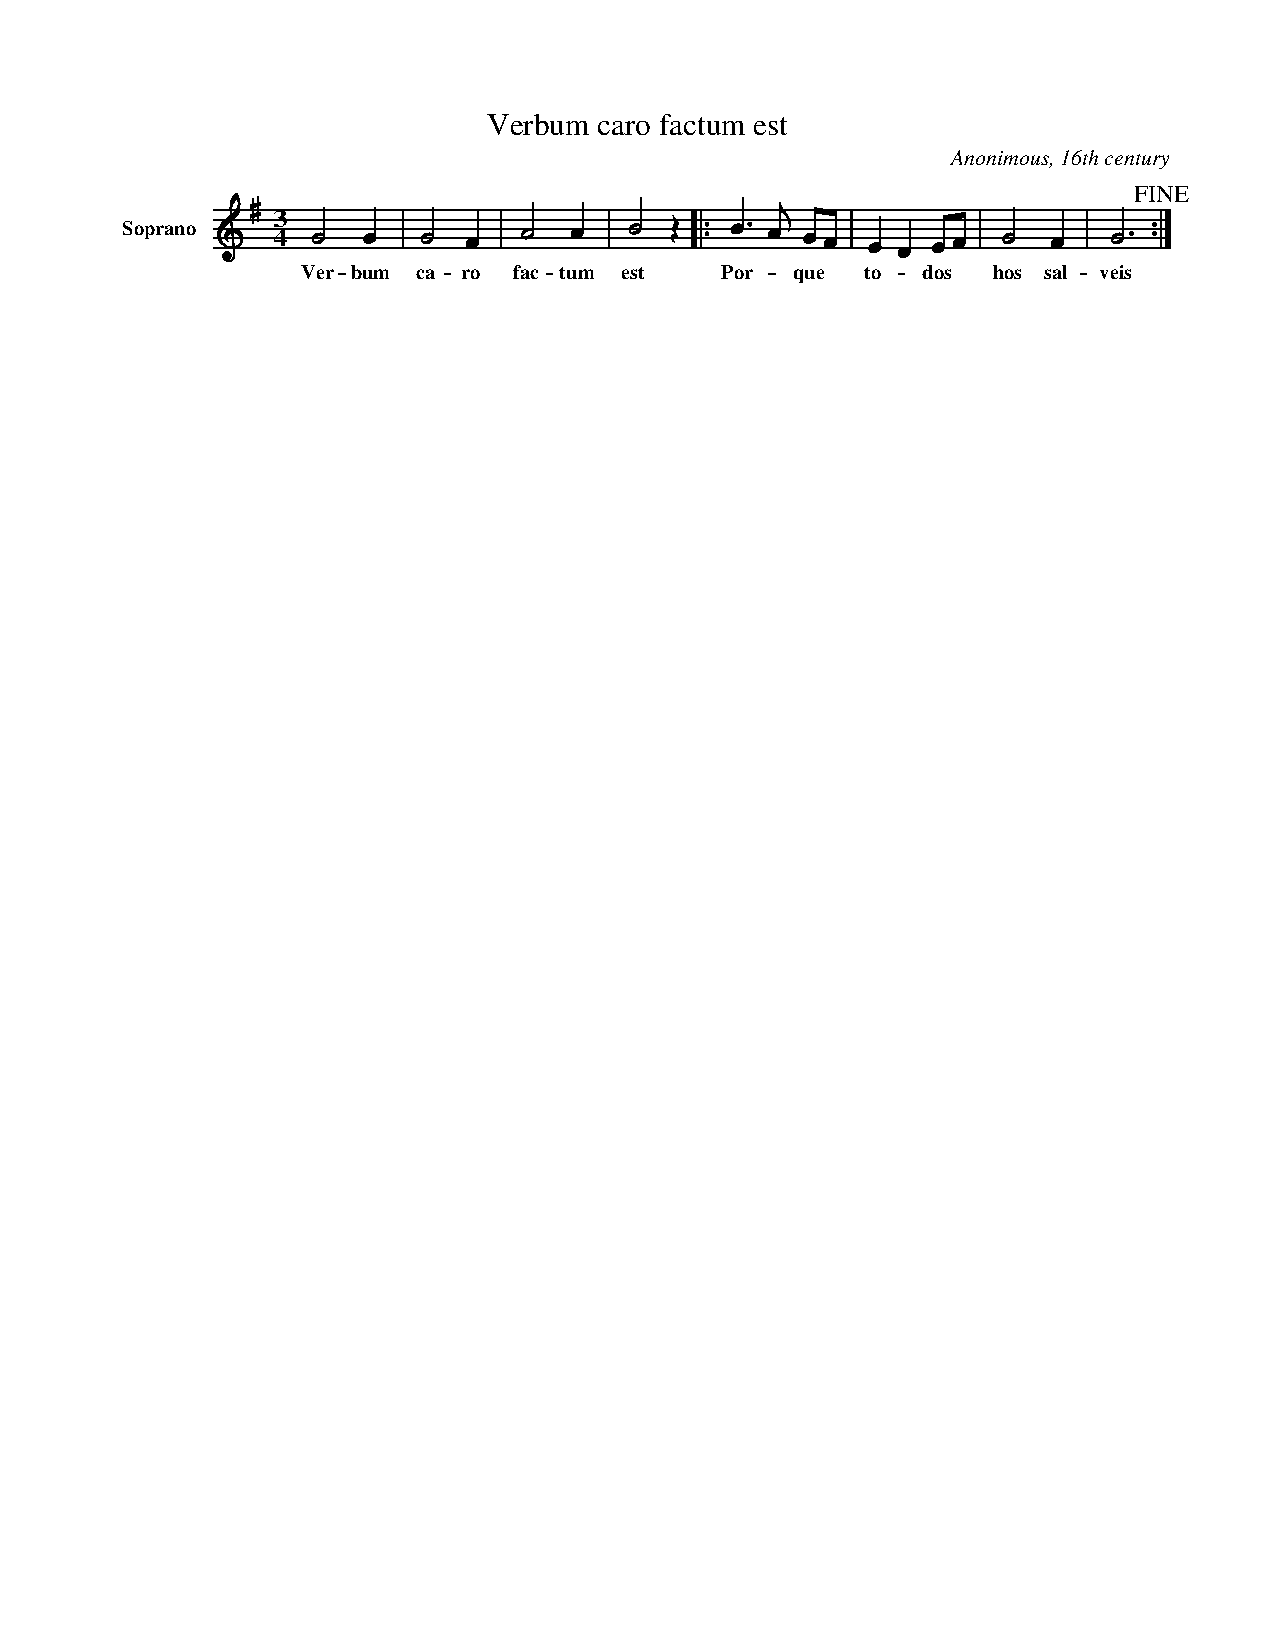
\includegraphics[width=0.8\textwidth, clip=true, trim = 0mm 230mm 0mm 17mm]{img/101.pdf}
  \caption{\abc{} example's generated score}
  \label{fig:abc_example}
\end{figure}

There are many \abcpt{}s and, among them, the most popular are the typesetter
\abcmtops{}~\cite{abcm2ps:Online} and the \midi{} creator \abctomidi{}~\cite{abc2midi:Online}. The
first translates music written in \abc{} into customary sheet music scores in PostScript or SVG
format. The latter converts an \abc{} file into a \midi{} file.

\subsection{LilyPond}

GNU LilyPond\cite{lilypond:Online} is a computer program and file format for music engraving. It
formats music beautifully and automatically, and has a friendly syntax for its input files. It is
Free Software, this is, open source. One of LilyPond's major goals is to produce scores that are
engraved with traditional layout rules, reflecting the era when scores were engraved by hand.

Although there are some small similarities to \abc{}, there are significant differences, starting
with their intent. \abc{}'s original purpose was to create a simple means of sharing folk tunes that
could be read as text and sent as email. Besides, it is a music notation standard, not a software
package. LilyPond is a software with the intent of creating printed musical scores that match the
best hand engraved musical scores of the past.

The similarity between \abc{} and LilyPond is in the means of specifying notes in a musical score,
this is, through the letters \emph{A} to \emph{G}.

LilyPond has a much more ambitious goal than \abc{}, therefore the markup language for its source
file can quickly become complex if the goal is to combine, for instance, melody, tab, chords, chord
diagrams and lyrics.

Listing \ref{lst:verbum_s1_p1_ly} illustrates the same example used for \abc{} using LilyPond
notation and figure \ref{fig:verbum_s1_p1_score_ly} its corresponding score.\\

\lstinputlisting[caption={LilyPond Example},label={lst:verbum_s1_p1_ly},captionpos=t,abovecaptionskip=-\medskipamount]{misc/verbum_s1_p1_ly.tex}

\vspace{-0.25cm}
\begin{figure}[htb]
  \centering
  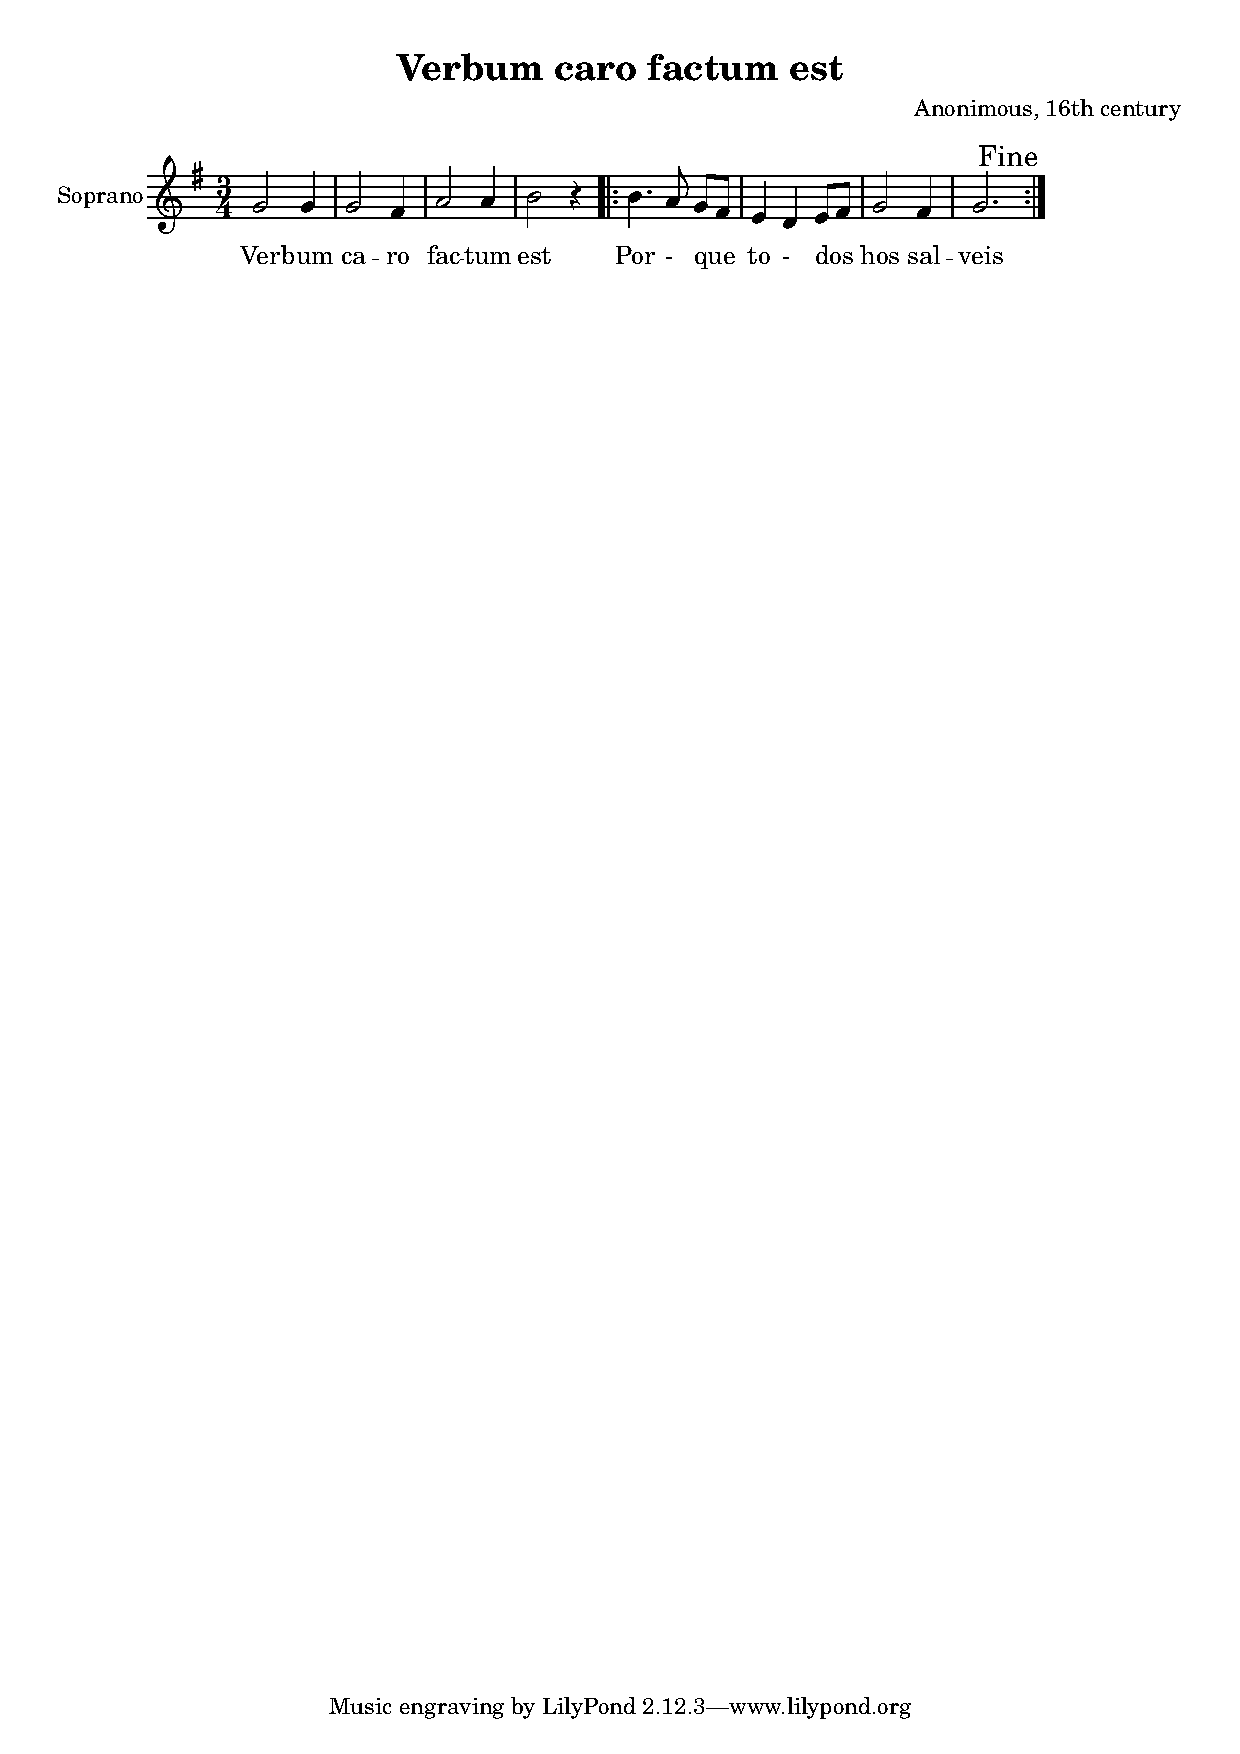
\includegraphics[width=0.8\textwidth, clip=true, trim = 9mm 250mm 9mm 6mm]{img/verbum_s1_p1_ly.pdf}
  \caption{LilyPond example's generated score}
  \label{fig:verbum_s1_p1_score_ly}
\end{figure}

\subsection{MusicXML}

MusicXML\cite{musicxml:Online} is an XML-based file format for representing Western musical notation
designed for notation, analysis, retrieval, and performance applications. The format is proprietary,
developed by Recordare LLC, but fully and openly documented, and can be freely used under a Public
License.

MusicXML was designed from the ground up for sharing sheet music files between different
applications, and for archiving sheet music files for use in the future. Its files are readable and
usable by a wide range of music notation applications, now and in the future. MusicXML complements
the native file formats used by Finale~\cite{Finale:Online} and other
programs~\cite{Sibelius:Online}, which are designed for rapid, interactive use.


\section{Internal Representation}
The representation of musical information is an area of research that has been receiving
contributions throughout time and it's not expected to be a consensus about a universal structure.

One of the most influent matters in making such representations is their final purpose. There are
different intentions, such as music rendering, play back, printing, music analysis, composition,
among others. The scope of this thesis includes only music rendering and analysis, therefore the
representation will have a well defined orientation which will not take into account additional
components that would benefit, for instance, composition tasks.

There are many models, data structures, paradigms, techniques, systems and theories proposed by many
authors~\cite{Brinkman1984,Buxton1978,Bilmes1992,Smaill1993,Wiggins1989,Dannenberg1993} and none can
be labeled as \emph{the perfect} representation, as there will never be a closed definition of
music and it is still difficult to represent all aspects of music.

% As will be explained in section \ref{sec:abc_dt}, this work presents a Perl module called \abcdt{},
% which can be viewed as a \ac{DSL} embedded in Perl. It processes some input information and returns it.
% The input information is parsed and an \ac{IR} is generated. That representation
% guides how the processing will be done. So, it is important to establish its structure, as it will
% determine how an \abc{} tune may be processed.

This dissertation's aim is to obtain a structure that allows the easy manipulation of music in a
computer. That structure should be compliant with a variety of tasks regarding music rendering and
analysis, such as, representing pitch and determining intervals from them, and obtaining all musical
elements that occur in a specific musical moment. Most importantly, it must allow the reconstruction
of the original \abc{}, in other words, it must contain all the original information including the
order of each element.

Next, a discussion on two topics is made: the pros and cons of sequential vs. hierarchical
representations and melody vs. harmony representations. The latter is mentioned again in section
\ref{sec:parse}.

\subsection{Sequential vs. Hierarchical}

The most used structures for music representation are the sequential and hierarchical structures.

\subsubsection*{Sequential}

In the beginning, computer music systems represented music as a simple sequence of notes. It was a
simple approach, thus making it difficult to encode structural relationships between notes, such as
enveloping a group of notes in order to apply some kind of property.

For instance, \midi{}~\cite{midi:Online} has no mechanisms for describing new structural
relationships.  However, \midi{} has a number of predefined structures. There are 16 channels, which
effectively form 16 groups of notes. Each group has a set of controllers such as volume and
pitch-bend. This gives \midi{} a limited 2-level structure.

The sequential structure refers to a sequence of any kind of musical component, usually indexed by
ordinal position rather than time. For instance, a musical element, such as a measure bar, is
referred as the fourth element rather than an element at time 5.7 seconds or at musical offset 3,
corresponding to the length of 3 quarter notes.

Many groupings of interest in music are likely to exhibit this property of strict ordering - most
melodies, for example, are monophonic. An analysis task's efficiency may improve when dealing with
this kind of structure.

\subsubsection*{Hierarchical}

It is widely accepted that music is best described at higher levels in terms of some sort of
hierarchical structure~\cite{balaban1987music}. This kind of structure has the benefit of isolating
different components of the score, therefore allowing transformations, such as tempo or pitch, to be
applied to each of them individually. It also represents a set of instructions for how to put the
score back together, hence allowing to reassemble it as it was.

Musical events can spread behavior to other events through the binary relation \textit{part-of},
which denotes relations like "measures part-of phrase". They can also inherit behavior and
characteristics from other events through the \textit{is-a} relation, which designates relations
like "a dominant chord being a special kind of seventh chord"~\cite{Honing1993}.

There are other kinds of relations that are needed as well in a hierarchical representation.
Honing\cite{Honing1993} suggests:

\begin{itemize}
  \item Binary:
    \begin{itemize}
      \item \textbf{associative:}
        e.g.: "A theme with its variations"
      \item \textbf{functional:}
        e.g.: "The function of a particular chord in a scale"
      \item \textbf{referential:}
        e.g.: "A theme referring to a previously presented or already known motif"
    \end{itemize}
  \item N-ary:
    These relations can structure more complex types of relation.\\
    e.g.: "the dependency of a certain chord on scale, mode and the context in which it is used is a
    ternary relation"
\end{itemize}

A single hierarchy scheme is not enough because music frequently contains multiple hierarchies, for
instance, a sequence of notes can belong simultaneously to a phrase marking and a to section (like a
movement). So the need of a multilevel hierarchy appears. There are some other possible hierarchies:
voices, sections (movement, measure), phrases, and chords, all of which are ways of
grouping and structuring music.

A few representations have been proposed~\cite{Dannenberg1990,Brinkman1984} that support multiple
hierarchies through named links relating musical events and through instances of hierarchies. And
others where tags are assigned to events in order to designate grouping, such as, all notes under a
slur.

\subsection{Melody vs. Harmony}

In polyphonic music there are materials besides melody that are combined in a score: rhythm and
harmony. Those three (melody, rhythm and harmony) determine the global quality of a
score~\cite{benward2003music} and their combination is usually called a texture. When there's only
one voice (melody), accompanied or not by chords, it is called monophony, but when there's two or
more independent voices, it is called polyphony.

The study of independent melodies is relatively simple compared to the analysis of polyphony. Each
voice moving through the horizontal dimension creates other effects by overlapping with notes in
other voices. The necessity for representing these vertical structures arises so that the harmonic
motion can be analysed.\\

Four suggestions of representations arise from this discussion: \partwise{}, \timewise{} and
\emph{hybrid} and \sourcewise{}.

\subsubsection{Part-wise}

The \partwise{} representation expresses a score by part (voice, instrument). So each part contains
many tuples (voice , \abcelements{}). Each \abcelement{} belongs to the specified voice. See example
\ref{ex:partwise}.

\begin{program}
  score $\rightarrow$ part*\\
  part $\rightarrow$ (voice, abc\_element*)\\
  \caption{\emph{Part-wise} representation}
  \label{ex:partwise}
\end{program}

This representation is best suited for melodic studies, considering that it is possible to directly
obtain all \abcelements{} belonging to a voice.

\subsubsection{Time-wise}

The \timewise{} representation expresses a score by time (musical moment), this is, by the offset of
the elapsed time. So each musical moment contains many parts. A part is a tuple (\emph{time offset}
, \emph{voice} , \abcelement{}). See example \ref{ex:timewise}.

\begin{program}
  score $\rightarrow$ musical\_moment*\\
  musical\_moment $\rightarrow$ part*\\
  part $\rightarrow$ (time\_offset, voice, abc\_element)
  \caption{\emph{Time-wise} representation}
  \label{ex:timewise}
\end{program}

This representation is best suited for harmonic studies, considering that it is possible to directly
obtain all musical events that occur in a specific moment in time.

MusicXML allows the representation of both time and part dimensions in two separate schemas. The
\partwise{} schema represents scores by part/instrument and the \timewise{} schema by time/measure.

\subsubsection{Hybrid}

The \emph{hybrid} representation derives from the need to solve an issue related with the
variability of a score's texture. This is, a score may have different densities of notes per part
and it is required that all events occurring at the same time are vertically aligned.

So, Brinkman~\cite{Brinkman1984} suggests a solution that uses a linked representation of a sparse
matrix. Each row of the latter references a part and each column the offset of the elapsed time,
which would enable traversing the score in any direction required (vertical or horizontal). Thus,
attaining a perception of the context of what's happening in a specific part, a feature that can't
be achieved when dealing with representations with only one dimension. Moreover, it makes the task
of score segmentation by part or time easier.

\subsubsection{Source-wise}

The \sourcewise{} representation expresses a score as it is parsed from the \abc{} file. So a score
is an ordered list of tuples (\abcelement{} , \context{}). The \context{} keeps record of an
\abcelement{}'s contextual information, this is, it keeps track of the current time offset, the
current voice, among other information (this \context{} is explained in more detail in section
\ref{sec:abcdt_rules}). See example \ref{ex:sourcewise}.

\begin{program}
  score $\rightarrow$ (abc\_element , context)*\\
  context $\rightarrow$ (current\_time, current\_voice, ...)
  \caption{\emph{Source-wise} representation}
  \label{ex:sourcewise}
\end{program}

This representation is best suited for rewriting purposes, considering that the actual order of
\abcelements{} is the same as in the original \abc{} file. It's also best for generic processing
where there's no need for a specific representation.


\subsection{Summary}

Two structures most commonly approached by researchers for representing music were discussed:
sequential and hierarchical. However, the decision of which structure type one should choose relies
on the purpose the \ac{IR} will have, such as, rendering of music, printing, music analysis,
composition, etc. This is, it relies in how many and what kind of questions are to be made to it.

A sequential structure may benefit certain tasks where a fast and simple traversal and/or a strict
ordering of its elements are required.

A hierarchical structure allows to isolate different components of a score and establish relations
between them. These are obvious advantages, although its traversal requires more advanced
techniques.\\

Regarding the horizontal and vertical dimensions of polyphonic music, four representations were
suggested. A \partwise{} representation is best suited for melodic studies, \timewise{} for harmonic
studies, \emph{hybrid} for both and \sourcewise{} for generic processing.

The most relevant disadvantage of the first three representations is that they don't maintain the
original order of elements. For instance, in \abc{}, it is common to write a part alternately with
other parts like (voice A, voice B, voice A, voice B). Meaning that a fragment of part A's music is
written first, followed by a fragment of part B, then another fragment from voice A and another from
voice B. When representing a score oriented to a vertical axis, the order in which each element is
written in the source file is lost, thus invalidating tasks like re-rendering \abc{} tunes.

% An assessment is taken after a, not so thorough, research on representations and their pros and
% cons: sequential and hierarchical structures are more suited to horizontal readings and tasks such
% as re-rendering an \abc{} tune, since they preserve the original order of the elements.

% Whereas, structures like sparse matrices grant both horizontal and vertical readings. Such
% structures provide a representation better suited to purposes requiring a quick access to vertical
% events on a score. Yet, it does not maintain the original order of elements. For instance, in
% \abc{}, it is common to write a part alternately with other parts like (voice A, voice B, voice A,
% voice B). Meaning that a fragment of part A's music is written first, followed by a fragment of part
% B, then another fragment from voice A and another from voice B. When representing a score oriented
% to a vertical axis, the order in which each element is written in the source file is lost, thus
% invalidating tasks like re-rendering \abc{} tunes.

A perfect representation would be one that is sufficiently generic and complete to be useful
in different analytic tasks in many styles of music~\cite{Honing1993}, like expressing common
abstract musical patterns.


\section{Projects and Tools}
\label{sec:projects}
In this section some of the most relevant projects and tools being developed or used at the moment
are discussed\footnote{A more extensive list of \abc{} software may be consulted in
http://abcnotation.com/software\#linux}.

\begin{description}
  \item[\textbf{abcm2ps}]~\cite{abcm2ps:Online}
    A command line program which translates music written in \abc{} music notation into customary
    sheet music scores in PostScript or SVG format.

    It is based on \texttt{abc2ps} 1.2.5 and was developed mainly to print Baroque organ scores that
    have independent voices played on multiple keyboards and a pedal-board. The  program has since
    then been extended to support various other notation conventions in use for sheet music.
    Moreover, it is now one of the most complete \abc{} implementations.

    It is developed in C language and the author, an organist and programmer called Jean-François
    Moine, releases “stable” and “development” versions of his program. As of this
    writing\footnote{\today}, the stable release is 6.6.22 and the development release is 7.6.0.
    Since release 7.2.1, \abcmtops{} tries to follow the \abc{} standard version
    2.1\footnote{http://abcnotation.com/wiki/abc:standard:v2.1}.

  \item[\textbf{abc2midi}]~\cite{abc2midi:Online}
    A program that converts an \abc{} music notation file into a \midi{} file.

    It is part of the abcMIDI package, which includes other utility applications.

    The program was developed in C language by James Allwright in the early 1990s and has been
    supported by Seymour Shlien since 2003. It contains many features, such as expansion of guitar
    chords, drum accompaniment, and support for micro tones which do not exist in other packages.

  \item[\textbf{tclabc}]~\cite{tclabc:Online}
    A \emph{tcl}\footnote{Tcl is a scripting language created by John Ousterhout. It is commonly
    used for rapid prototyping, scripted applications, GUIs and testing. Tcl is used on embedded
    systems platforms, both in its full form and in several other small-footprint versions.}
    extension which permits ABC tunes parsing and editing.

    \begin{itemize}
      \item the \abc{} tunes are converted into an \ac{IR} suitable for many tcl operations, without
      losing the original tune information;
      \item most of the \abc{} specification is supported;
      \item the headers and tune symbols may be changed in many ways;
      \item transposition is done automatically when changing the key signature;
      \item bars may be automatically inserted;
      \item \midi{} files may be imported and exported;
      \item partial dump/include solves the selection copy/paste functions;
      \item \midi{} input and output are supported on many systems;
    \end{itemize}

  \item[\textbf{Music21}]~\cite{music21:Online}
    A Python-based toolkit for computer-aided musicology.

    Music21 is a set of tools for helping scholars and other active listeners answer questions about
    music quickly and simply.

    Music21 builds on preexisting frameworks and technologies such as Humdrum, MusicXML, MuseData,
    \midi{}, and LilyPond, but Music21 uses an object-oriented skeleton that makes it easier to
    handle complex data. At the same time, Music21 tries to keep its code clear and makes reusing
    existing code simple.

    Applications of this toolkit include computational musicology, music informations, musical
    example extraction and generation, music notation editing and scripting, and a wide variety of
    approaches to composition, both algorithmic and directly specified.

    It also has a large corpus of musical scores in many formats, including \abc{} and MusicXML.

  \item[\textbf{abctool}]~\cite{abctool:Online}
    A Python script that manipulates music files in \abc{} format.

    It's mostly useful for people working on the command line and/or editing \abc{} directly in an
    editor. It relies on external programs for certain tasks like converting into PostScript or
    transposing.

    Its main features are reading from standard input or file, outputting to standard output
    (PostScript, PDF or \midi{}), viewing (using \abcmtops{} and \texttt{gv}), transposing,
    translating chord names to Danish/German, and removing chords and fingerings.

    It is open source, developed by Atte André Jensen and released under GPL.

  \item[\textbf{Haskore}]~\cite{hudak1996haskore}
    Haskore is a set of Haskell modules for creating, analyzing and manipulating music.

    The formal approach used in this project is very elegant and powerful and is a very good
    studying resource. Nevertheless, when one wants to process existing \abc{} music, there are many
    details that don't fit in Haskore model like slurs, dynamics, microtones. In order to process
    them, those elements must be forgotten or drastic changes to the model must be introduced.

  \item[\textbf{EasyAbc}]~\cite{easyabc:Online}
    An open source \abc{} editor for Windows, OSX and Linux.

    It uses \abcmtops{} and \abctomidi{} and it has a rich features list. Most notably, it can
    import MusicXML files and export tunes in SVG format. It is published under the GNU Public
    License and was developed by Nils Liberg.

  \item[\textbf{abcpp Preprocessor}]~\cite{abcplus:Online}
    A simple yet powerful preprocessor designed for, but not limited to, \abc{} music files.

    It was written to overcome incompatibilities between \abc{} packages, and to facilitate writing
    portable and more readable \abc{} files. A preprocessor is a program that modifies a text file,
    according to commands contained in the file.

    It provides:
    \begin{itemize}
      \item conditional output;
      \item exclude or include parts of a piece according to specified conditions;
      \item define macros, i.e. symbols and sequences of customized commands;
      \item rename commands, symbols, and notes;
      \item include parts of other files.
    \end{itemize}

  \item[\textbf{ABCp}]~\cite{abcp:Online}
    A parser for the \abc{} music notation.

    It is a C library that interprets \abc{}. It is released as open source, under the terms of the
    BSD license, and may be used in both free and commercial software.

    ABCp has been designed with the following requirements in mind:
    \begin{itemize}
      \item to be able to handle the \abc{} 2.0 standard as well as previous standards and the
      extensions introduced by the most widely used tools (\abcmtops{}, abcMIDI, ...);
      \item to be fast;
      \item to be small: there must be a fair trade-off between size and functionalities;
      \item to be easily embeddable: no big restriction on the programming language to use;
      \item to be usable: no complex API or class hierarchy to remember.
    \end{itemize}

  \item[\textbf{Music::Abc::Archive}]~\cite{music_abc_archive:Online}
    A Perl module to parse \abc{} music archives.

    \abc{} music archives contain songs in the \abc{} format. This module encapsulates the \abc{}
    archive and individual songs so they may be managed more easily by Perl front-ends.

\end{description}

Some of the tools and projects presented were very relevant: \texttt{abctool} is a simple command
following \unix{}'s philosophy; \abctomidi{} and \abcmtops{} deal with processing real world \abc{}s,
but have specific purposes; \texttt{Music21} has similar goals and has a very powerful and complex
object oriented modules for music processing; \texttt{Haskore} is very flexible and elegant but
can't deal with real world \abc{} details.


\section{Corpora}
In order to calculate the difference between what is considered a pattern, assess what is expected,
calculate similarities between scores or generate statistics there must exist some example cases.

Those example cases are called corpus and in this dissertation's case it is a specific corpus (a
musical corpus) which contains rich metadata regarding musical scores. The knowledge generated by
the analysis of the corpus may be shared by many tools through a richer combination of tools.

The corpus can be used as testing material for the toolkit, for instance, a tool that validates an
\abc{} score's syntax needs either flawless examples or examples with deliberately typed errors to
guarantee that it works as it's supposed to. Also, it can be used to train systems that learn from
data, for instance, a system that is trained with a set of scores in order to learn how to identify
certain music aspects, such as the style.

% Other uses for the corpus include:
% \begin{description}
%   \item[Testing material for the toolkit] \hfill \\
%     A tool that validates syntax needs either flawless examples or examples with deliberately typed errors
% to guarantee that it works as it's supposed to. 
%   \item[Training systems that learn from data] \hfill \\
%     A system that is trained with a set of scores in order to learn how to identify certain music
%     aspects, such as the style.
% \end{description}

\subsection{Building corpora}

This phase, according to existing literature on building corpora~\cite{Atkins1992,
wynne2005developing,teseandre} (plural of corpus), consists of planning the whole process and
annotating them.

\subsubsection*{Planning}

In this step decisions have to be made so that the remaining steps may take place. They consist in
defining the quantity of scores that will be added to the corpus, selecting the scores that should
be added (according to their use and availability), defining the intermediary formats and
conventions to be used in the processing pipeline, defining if and what annotations should be
included in the corpus and finally, defining in which formats the corpus should be available and how
should the analysis tools interface with them.

% \begin{itemize}
%   \item Define the quantity of scores that will be added to the corpus;
%   \item Select the scores that should be added, according to their use and availability;
%   \item Define the intermediary formats and conventions to be used in the processing pipeline;
%   \item Define if and what annotations should be included in the corpus;
%   \item Define in which formats the corpus should be available and how should the analysis tools
%     interface with them.
% \end{itemize}

% \subsubsection*{Getting permissions}
% 
% Scores will be gathered from public domain as they are not subject to copyright.

\subsubsection*{Gathering scores}

\abc{} notation has become very popular since its introduction, and nowadays thousands of tunes
exist in electronic format. Scores, as in a music consisting of multiple voices, exist in a lesser
number because the features that allow the writing of polyphony were only added to the standard much
later, yet it is an ever growing culture. However, a previous parsing and reformatting might still
be needed in order to process them efficiently.

\subsubsection*{Annotating scores}

In order to improve the usefulness of a corpus for a richer and more rigorous statistical analysis,
it might be subject to the process of annotation. It consists in applying some sort of structural
representation to act as a blue print of the original text and to provide additional interpretative
information.

% Yet, the use of annotations is not always the best approach. Susan Hunston, in \textit{Corpora in
% Applied Linguistics}~\cite{hunston2002corpora} states that the kind of questions that are usually
% asked to a corpus tend to be limited rather than the questions that can be asked. This happens
% because the categories used to annotate a corpus are frequently determined before any analysis is
% done. Thus, as stated before, a careful planning has to be made.


\subsection{What can be analysed} 

It's desired that a set of tools for statistical calculation is built. To make that possible a large
set of corpora must be built, so that statistical analysis and hypothesis
testing\footnote{Hypothesis testing is the use of statistics to determine the probability that a
given hypothesis is true.} can be performed and from the results extract valuable information.

The corpus may be used for finding sets of vertical patterns that occur in a large number of scores
in the corpus\cite{Conklin2002}, measuring rhythmic similarity (the repetitive nature of the music)
with manual annotations to the corpus\cite{antonopoulos2007music}, identifying trends and changes
throughout a historical time period through cluster analysis\cite{albrechtemergence}, among many
other uses.

% Some examples of what can be analysed in musical corpora:
% 
% \begin{itemize}
%   \item Find sets of vertical patterns that occur in a large number of scores in the
%     corpus\cite{Conklin2002};
%   \item Find significant statistical differences between melodies of folk music from different
%     countries\cite{chai2001folk};
%   \item Display multiple excerpts from a collection of scores, such as all of the cadences, without
%     human intervention and editing\cite{Knopke};
%   \item Measure rhythmic similarity - the repetitive nature of the music - with manual annotations
%     to the corpus\cite{antonopoulos2007music};
%   \item Study norms of behavior for documenting relationships between accents and harmonic structure
%     in common-practice music, and the role of notational variants in identifying scribes and
%     composers\cite{Ariza};
%   \item Identify trends and changes throughout a historical time period through cluster
%     analysis\cite{albrechtemergence}.
% \end{itemize}

\subsection{Existing Corpora} 

There are many existing musical corpus available in the Internet. A large corpus will be assembled
ranging from \abc{} corpus, to \midi{}, MusicXML and still LilyPond. 

The corpus format may vary depending on what the tools can read and process, for instance, if
\midi{} transformations are implemented then a \midi{} corpus has to exist as well. As this
dissertation's focus is \abc{}, the main format will also be \abc{}.

Here are some of the websites and packages from where they'll be gathered:

\begin{description}
  \item[http://abcnotation.com/browseTunes] \hfill \\
    Around 350,000 tunes available as \abc{} or \midi{} sound files;
  \item[http://thesession.org/] \hfill \\
    Around 11,000 tunes available as \abc{} or \midi{} sound files;
  \item[http://moinejf.free.fr/abc/index.html] \hfill \\
    \abc{} organ pieces;
  \item[http://www.classicalarchives.com] \hfill \\
    Around 14,000 \midi{} sound files;
  \item[http://abc.sourceforge.net/NMD/] \hfill \\
    Around 1000 \abc{} files;
  \item[Music21 corpus package] \hfill \\
    A collection of approximately 10,000 works including a complete collection of the Bach Chorales,
    numerous Beethoven String Quartets, and examples of Renaissance polyphony. The corpus includes
    \abc{}, MusicXML and Kern files.
  \item[http://wiki-score.org/] \hfill \\
    Modern editions written in \abc{} of unknown works buried in music archives.
  \item[http://www.mutopiaproject.org/] \hfill \\
    Sheet music editions of classical music in LilyPond.
\end{description}

\subsection{Summary}

A musical corpus will be built according to the needs of the toolkit. The initial need is for a
toolkit that reads and processes \abc{} notation, so the main focus will be to build an \abc{}
corpus.

A careful planning on how to build the corpus plays an important part on determining the quality and
quantity of tasks that can make use of it. Such planning strongly affects the final results an
\abcpt{} can produce.



  % How am I going to discover it?
  % This study was based on the approach of…
  % This approach was chosen because…
  % It was likely to achieve the project aims by…
  % Others have used this method to…
  \chapter{ABC::DT and ABC processing tools}
  \label{sec:abc_dt}

A typical \abcpt{} follows a traditional compiler's structure:

\begin{enumerate}
  \item \textbf{Parse \abc{} input}\\ \hfill
    The \abc{} parser generates an internal representation (\ac{IR}) to be transformed in the
    following stage.
  \item \textbf{Transform the generated representation}\\ \hfill
    The \ac{IR} is transformed.
  \item \textbf{Generate the output}\\ \hfill
    An output of the transformed \ac{IR} is generated.
\end{enumerate}

Figure \ref{fig:process_stages} illustrates an \abcpt{}'s architecture.

\begin{figure}[H]
  \centering
  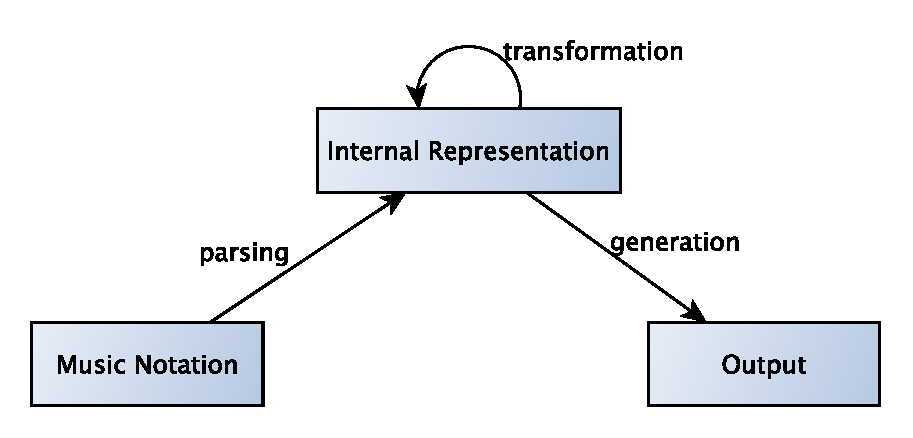
\includegraphics[width=0.8\textwidth]{img/abc_dt.pdf}
  \caption{\abcpt{}'s architecture}
  \label{fig:process_stages}
\end{figure}

In order to be able to create new \abcpt{}s in the most simple and compact way possible, a \ac{DSL}
called \abcdt{} was created as well as its processor, in which:

\begin{enumerate}
  \item The parsing process is invoked automatically, considering the parser is constant and
  independent of the intended transformation, thus being common to every \abcpt{}.
  \item The \ac{IR}'s transformation is described by a set of rules specified by the user (referred
  to as \abcdtrules{}). Each rule is composed by the pair \emph{actuator $\Rightarrow$
  transformation}, where the \actuator{} describes the \ac{IR}'s part to be processed and the
  \transformation{} is the set of instructions to be applied to that part.
  \item The output generation in \abc{} format is provided by default. The default function is the
  identity function - \toabc{}.
\end{enumerate}

The details of \abcdt{}'s implementation will be described next, following the three stages of the
architecture aforementioned.

\section{Parse ABC Input}
\label{sec:parse}

As was previously stated in the introduction, an \abcpt{} must be able to deal with real \abc{}
music. Therefore, the \abc{} parser has to be robust, i.e., it must be able to expect cases that it
doesn't recognize.

The main options for building the parser were: to build it from scratch; to reuse an existing parser
from robust programs like \abcmtops{}~\cite{abcm2ps:Online} or \abctomidi{}~\cite{abc2midi:Online}
and adapt it to the requirements; or to use directly one of the aforementioned programs' parsers.

Since building a robust parser is very time consuming, the first solution was discarded. The second
option would raise problems when adapting it to newer versions. So, using \abcmtops{} or
\abctomidi{}'s parser was the natural choice. The program chosen was \abcmtops{} for the reasons
that are explained in the following section.

\subsection{\abcmtops{} parser's features}

\abcmtops{} is one of the most widely used programs for working with \abc{}, not just as a
standalone software but as part of many applications. This fact implies that it's not a piece of
software that was casually made. It was designed to process \abc{} in the best way possible,
therefore its quality is acknowledged.

It is actively maintained and well documented which facilitates the analysis of the structures its
parser generates. Moreover, its author, Jeff Moine, was and still is a preponderant influence for
the evolution of the \abc{} notation and standard. Its parser is also used in other Moine's tools
like \tclabc{}~\cite{tclabc:Online}.

The \ac{IR} generated by its parser follows the sequential structure type and it's \sourcewise{}. In
other words, each element captured by the parser is simply appended to an ordered list, resulting in
a sequence of \abcelements{} in the same order they are parsed. An element is any component existing
in \abc{}, from the header information - like the key or initial meter - to a note, bar, a tuplet or
lyrics.

Given that \abcmtops{} was designed to print \abc{} scores, its \ac{IR} (\sourcewise{}) is not well suited
for music analysis or composition purposes. Still, it can be easily transformed into different views
of the same representation. For instance, a \timewise{} \ac{IR} could be a set of monophonic voices,
which could be used to describe relationships between vertical musical entities on a polyphonic
score.

% Therefore, it lacks all the benefits inherent to an hierarchical
% representation, such as, inheriting behavior and characteristics between musical events.
As the aim of this dissertation is to build a toolkit based on scripts, the sequential structure is
very appropriate since the sequence of elements that it provides can be easily mapped to an
\emph{array} or a \emph{hash}. These data types are part of the common, yet powerful, data types of
a scripting language like Perl, which is the kind of approach that's intended.

\subsection{From \abcmtops{} parser's IR to Perl}

At this point, it was necessary to define a strategy to implement the first stage (\emph{Parse
\abc{} Input}).

It consists in selecting the best and most robust tool that processes \abc{}, isolate its parser and
finally add a traversal function that serializes\footnote{Serialization is the process of
translating data structures into a format that can be stored and resurrected later in the same or
another computer environment.} the \ac{IR}'s structure so that it can be evaluated by Perl into a Perl
structure.

Perl is the developing language being used and, since it supports reflection\footnote{Reflection is
the ability of a computer program to examine and modify the structure and behavior (specifically the
values, meta-data, properties and functions) of an object at runtime.}, it provides the ability to
evaluate a string as if it were a source code statement at runtime.

So \abcmtops{} is the tool selected to have the parser extracted. Its parser is implemented in C, so
the structure that it generates is a list of C data structures. Therefore, a C program - called
\abctoperl{} - was created. It uses \abcmtops{}' parser to parse an \abc{} file into a C structure,
then it translates that structure into a serialized Perl \emph{hash} which is then printed to the
standard output.

In short, \emph{Parse \abc{} Input} stage is comprised of a Perl serialization of the structure
generated by \abcmtops{}' parser (\abctoperl{}), followed by a Perl evaluation of the serialized
structure into a Perl \emph{hash}. This way, a Perl structure that maps the original C structure is
obtained, which can be manipulated in the following stages.

Figure \ref{fig:parse_abc_input_stage} depicts the internal workflow of \emph{Parse \abc{} Input}
stage. \abctoperl{}'s workflow is represented by the group node '\abctoperl{}'.

\begin{figure}[htb]
  \centering
  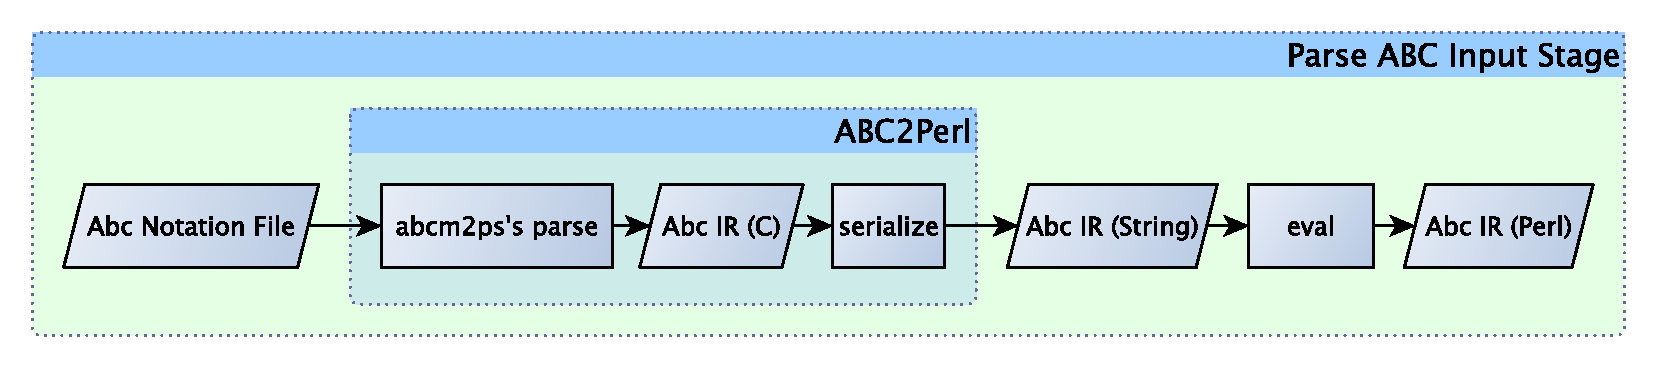
\includegraphics[width=\textwidth]{img/parse_abc_input_stage.pdf}
  \caption{\emph{Parse \abc{} Input} stage}
  \label{fig:parse_abc_input_stage}
\end{figure}

A simple mapping of the original C structure into a Perl one is being made. Hence the original order
and meaning are being kept. However, it could be possible to reorganize the structure to serve other
purposes. For example, representing it by part (\partwise{}) means that a specific part can be
accessed directly. Or representing it by elapsed time (\timewise{}) means that it is be possible to
directly retrieve all musical events that occur in a specific moment in time.

The approach being used in this strategy can be reused in other situations similar to this one where
a parser is needed and there already exists a powerful one. \abcdt{}'s parser update process is
facilitated due to its constituents being autonomous, which means that only those constituents need
to be updated to newer versions.

An Haskell specification of the serialized structure can be consulted in appendix
\ref{sec:abcm2ps_parser_ir}.

\section{Transform the generated representation}

This stage consists of making a traversal of the \ac{IR} generated in the previous stage and
applying a rule-based transformation to it.

The generic processing strategy is based on a structured processing of the \ac{IR}. It is possible
to process complex structures, like \abcmtops{}', if its processing is divided , i.e., if there are
many small surgical transformations done to its parts, and each individual result is composed into a
single one.  This approach has been successfully used, for instance, in the processing module of XML
documents, XML::DT~\cite{tesejj}, attribute grammars~\cite{paakki1995attribute} and
\emph{Stratego}~\cite{Stratego:Online}.  This strategy is called DT (\emph{Down Translate}) and it's
basically a depth traversal of the structure where each individual element may have a specific
transformation associated.

The global transformation consists in specifying a set of rules. Those rules associate smaller
transformations to very specific points in the \ac{IR} and any point not covered in the rules is
kept unchanged, triggering the default transformation.

In order to provide a systematic and efficient method to specify the rules, a \ac{DSL} called
\abcdt{} was created. It allows the user to specify, in Perl, the rules to be applied to an \abc{}
score. It's actually a Perl module that can be seen as a \ac{DSL} embedded in Perl. The set of rules
is called \abcdtrules{}.

In the following sections, \abcdt{}'s main processor algorithm (\dt{}) and \abcdtrules{} are going
to be explained in more detail.

\subsection{Processor Algorithm}

\abcdt{}'s main processor is called \dt{}. It admits an \abc{} file which is parsed using the
\abctoperl{} program described in the previous section. It also admits a table of \abcdt{} rules - a
dispatch table\footnote{A dispatch table is a table of pointers to functions or methods.} - in which
an \actuator{} is associated with a \transformation{}.

It performs a traversal guided by the \ac{IR} meaning that a full traversal is done and each \abc{}
element is processed sequentially. Each visited element is matched against the table of \abcdt{}
rules in order to find the \transformation{} to apply. Additionally, the \context{} for the current
element is calculated, which consists of the voice's id and name, the time elapsed until that
element, the meter, the key, among others. The \context{} grants a more complete control of what can
be processed, thus providing a richer semantic processing.

It's possible to define a default transformation to cover any \abcelement{} that doesn't match any
rule. This is achieved through the rule \emph{-default}. Moreover, if no default transformation is
explicitly defined, then there is the default's default transformation, which is the identity
function (\toabc{}).

\dt{}'s behavior resembles the one from the utility \awk{}\footnote{\awk{} is a pattern scanning and
processing language, typically used as a data extraction and reporting tool}~\cite{awk:Online}
considering that the latter's processing is based on a sequence of pattern-action statements. Each
processed file is transformed into a sequence of symbols. Each symbol is processed one at a time and
matched against all patterns, and for each pattern that matches, the associated action is executed.
In \abcdt{}'s case, only the most specific \actuator{} (pattern) has its \transformation{} executed.
This is explained in more detail in section \ref{sec:abcdt_rules}.

\dt{}'s default output is the concatenation of each individual \transformation{}'s result, which is a
string. Optionally, a \emph{-end} rule can be added to the rules which enables a general post
processing of the final result, hence, making possible to attain different output formats.

The algorithm just described is expressed in Algorithm \ref{alg:dt}.

\begin{algorithm}
  \KwIn{abc-file}
  \KwIn{rules: $[(actuator,transf)]$}
  $musicIR \gets$ abc2perl(abc-file) \hfill //parse\\
  \ForAll{$ elem \in musicIR $}{
     $context \gets$ recalculate current context\\
     $transf\gets \mbox{rule ∈ rules with best matching actuator \textbf{or} -default \textbf{or} \toabc{}}$\\
     $res \gets res$ ++ $transf(elem, context)$ \\
  }
  \Return{rules[-end] \textbf{or} $res$}
  \caption{\dt{}'s algorithm}
  \label{alg:dt}
\end{algorithm}

The rule-based structured processing strategy grants an easy and effective way to build tools that
make simple transformations, considering that most of the processing is done in the background, this
is, it's only needed to provide the description of what is to be changed.

% In order to define how the outcome of processing a symbol should be merged with others, the
% processor must know which processing strategy it must use. Thus, a table of strategies is needed
% and by default the processor uses the \texttt{STR} strategy which makes the string concatenation
% of the outcome of each symbol.\\
% Other strategies might be added to the table. For instance, a strategy that maps a set of
% symbols to a Perl structure so that it can be processed as a whole. Such a set might be
% difficult to process with the default strategy.

\subsection{ABC::DT Rules}
\label{sec:abcdt_rules}

A language with the ability to do descriptive/surgical processing, in the sense that a
transformation may be applied to a specific element, enhances the effectiveness of the tool to be
generated. That ability takes shape as an \abcdt{} rule. It is a correspondence between an
\actuator{} and a \transformation{}.

\subsubsection{Actuator}

\emph{Actuators} act as a query language for selecting specific \abcelements{} (e.g.: a note) or a
set of elements (e.g.: all elements that are defined in a particular context/state). They are
designed in a way that there is a natural notation for matching (testing whether or not an \abc{}
element matches a pattern).

An \actuator{} (pattern) specifies a set of conditions on an \abcelement{}. An element that
satisfies the conditions matches the pattern; an element that does not satisfy the conditions does
not match the pattern.

There's an undirected graph of \abcelements{} that guides the pattern matching process. That graph
dictates the priority an \actuator{} has over other \actuators{}, so that if there's more than one
match, the most specific \actuator{}'s \transformation{} is applied to the \abcelement{}. Figure
\ref{fig:pscom} illustrates the graph for the \emph{pscom} class, in which the \actuators{}
\emph{MIDI} and \emph{FORMAT} are both instances of \emph{pscom} and therefore are more specific.
\emph{Actuator} \emph{MIDI::channel}\footnote{\emph{MIDI::channel} is an abcMIDI command that
selects a melody channel (ranging from 1 to 16 channels)} is an instance of \emph{MIDI} and is more
specific than the previous \actuators{}. Example \ref{ex:pscom_example} shows an example of the
\emph{actuator matching} process' behavior when facing a situation where there are more than one
possible matches.\\

\begin{figure}[h!]
  \centering
  \graph
  [scale=0.7]{g1}
  {
    margin="0 0 0 0";
    pscom--MIDI
    MIDI--"MIDI::channel"
    MIDI--"..."
    pscom--FORMAT;
    FORMAT--staves;
    FORMAT--autoclef;
    FORMAT--"....";
  }
  \caption{ Undirected graph of the \emph{pscom} class }
  \label{fig:pscom}
\end{figure}

\begin{program}
  An \abc{} element representing the abcMIDI command \emph{\%\%MIDI channel} is being subject to
  the \actuator{} matching process.\\

  The set of rules passed to the processor contains the \actuators{} \emph{pscom}, \emph{MIDI} and
  \emph{MIDI::channel}.\\

  The \abcelement{} satisfies the conditions specified by all of the \actuators{}, therefore the
  most specific has to be chosen.\\

  The graph dictates that the most specific \actuator{} is \emph{MIDI::channel}, so it is the
  actuator selected.

  \caption{\emph{Actuator matching}}
  \label{ex:pscom_example}
\end{program}

An \actuator{} is comprised of one to three components, each separated by the characters
'\emph{::}'.

An \actuator{} with just a single component represents either: 1) an \abc{} state, 2) an
\abcelement{} type, 3) a specific \abcelement{}, or 4) one of the special \actuators{}
(\emph{-default} and \emph{-end}).

\begin{enumerate}
  \item The \abc{} state represents the context in which an \abcelement{} appears in the tune. It
  can be \emph{in\_global} (any element written between the tune's beginning and the header
  \texttt{X:}), \emph{in\_header} (any element written between the headers \texttt{X:} and
  \texttt{K:}), \emph{in\_tune} (any element written after the header \texttt{K:}) and
  \emph{in\_line} (any embedded element, i.e. written between the characters '[' and ']').

  \item The \abcelement{} type represents a class of elements, such as \emph{note} (a note or a
  chord), \emph{info} (any \abc{} header (\texttt{K:}, \texttt{V:}, ...)), \emph{pscom} (any
  formatting or abcMIDI command), \emph{tuplet} (an element that indicates that the following
  elements belong to a tuplet), \emph{gchord}, \emph{deco} (respectively, an accompaniment chord and
  a decoration/ornament which are associated with a \emph{note}, \emph{rest} or \emph{bar}).

  \item A specific \abcelement{} represents an instance of a class of \abcelements{}, such as
  \emph{staves} (an instance of the class \emph{pscom}; it's a particular formatting command),
  \emph{!ff!} (an instance of the class \emph{deco}; it's a dynamics, \emph{fortissimo}), \emph{V:}
  (an instance of the class \emph{info}; it's the header that indicates that the following music
  belongs to the voice specified).

  \item The special \actuator{} \emph{-default} describes how to transform uncovered \abcelements{}
  and the \actuator{} \emph{-end} enables a general post processing of \dt{}'s final result, hence,
  making possible to attain different output formats.
\end{enumerate}

An \actuator{} may have other components added: 1) an instance of an \abcelement{}'s class, 2) a
restriction on \abcelements{}.

\begin{enumerate}
  \item An instance of an \abcelement{}'s class may be added, such as \emph{MIDI::channel}
  (\emph{channel} is an instance of \emph{MIDI} (abcMIDI command)) or \emph{note::C}
  (\emph{C} is an instance of \emph{note}).

  \item A restriction (filter) on \abcelements{} may be added, such as \emph{V:Tenor::rest} (it
  selects any \emph{element} \emph{rest} that belongs to the voice with name \texttt{Tenor}),
  \emph{bar::gchord::FINE} (selects any \emph{gchord} with text \texttt{FINE} that is associated to
  a \emph{bar}) or \emph{in\_line::K:} (selects all \emph{K:} \emph{elements} whose \emph{state} is
  \emph{in\_line}, this is embedded headers).
\end{enumerate}

Due to the existence of different levels of detail, when an \abcelement{} matches more than one
\actuator{}, the most specific is the one chosen. This corresponds to the deepest selectable node in
the graph of \actuators{}.

A list of the currently available \actuators{} in \abcdt{} rules may be consulted in appendix
\ref{sec:abcdt_rules_actuators}.\\

In the future, another approach to \actuators{} specification is going to be investigated. What's
intended is a richer syntax for identifying \abcelements{}, one that uses path expressions to
navigate through an \abc{} tune and has a set of standard functions to help selecting
\abcelements{}. This approach should be very similar to \emph{XPath}'s\cite{XPath:Online}.

\subsubsection{Transformation}

A \transformation{} is specified by the user and it defines how each \abcelement{} should be
processed according to its internal values.

\abcdt{} requires that only \abcelements{} that need to be transformed are specified, meaning that
what is not explicitly specified also needs to be processed. The default function which processes
the latter is the identity function - \toabc{} - and it prints the contents of an \emph{element}
just as it was in the \abc{} source file. \toabc{}'s Perl implementation was inspired on
Jean-François Moine's \tclabc{}~\cite{tclabc:Online} \symdumpi{} function which dumps the original
\abcelement{}.  \abcmtops{} and \tclabc{} use the same parser and \ac{IR}, therefore \symdumpi{}
integration in \abcdt{} was made without major obstacles.

In addition to user specified functions, there is a set of default functions that help accomplish
certain tasks which would otherwise make more difficult the creation of \abcpt{}s.
Music21~\cite{music21:Online} has been developing a set of effective methods for music processing
which reveal an advanced state of maturity, therefore they have been a source of inspiration for
some of the created functions.

Most of these functions emerged from simple necessity when some of the \abcpt{}s (described in
chapter \ref{chap:abc_dt_by_example}) were being built . Many \transformations{} were becoming very
complex and were making the code very hard to read and maintain, therefore, some functionalities
being implemented became \abcdt{} default functions. Some of those functions may be consulted in
appendix \ref{sec:abcdt_functions}.

As was previously mentioned in this section, during \dt{}'s traversal, for every \abcelement{}
visited, the \context{} is calculated. This \context{} allows the user to access contextual
information of the tune at that moment. It includes the current voice's \emph{id} and \emph{name},
the \emph{time} elapsed until that moment, the \emph{meter}, the total duration a measure should
have (\emph{wmeasure}), the note's \emph{length}, and the \emph{key} along with some properties: the
number of sharp/flats (\emph{sf}), the \emph{exp} flag, the number of explicit accidentals
(\emph{nacc}), the \midi{} number for each explicit note in the key element (\emph{pits}) and the
code that identifies the accidental for each explicit note in the key element (\emph{accs}).

\subsection{ABC::DT's main features}

\abcdt{}'s main features are summarized as follows:

\begin{description}
  \item[Dispatch Table] \hfill \\
    \abcdt{} rules are defined by a correspondence between the \actuators{} and \transformations{}.
  \item[Rich Actuators] \hfill \\
    The set of \actuators{} is comprised of well structured elements in order to provide a precise
    \abcelements{} matching.
  \item[Higher-Order Processing] \hfill \\
    The \transformations{} are user specified functions, or the identity function (\toabc{}).
  \item[Systematic] \hfill \\
    In order to build an \abcpt{}, the user must define what and how is to be transformed.
  \item[Specify only the necessary] \hfill \\
    If no \actuator{} applies, the \emph{default} function is used.
  % \item[Processing strategies] \hfill \\
  %   There is a table of strategies. Each strategy defines how a transformation's output is to be
  %   merged with others.
\end{description}

\section{Generate the output}

In this stage, an output of the transformed \ac{IR} is produced.

By default, \toabc{} is the transformation applied to an \abcelement{}, therefore the output
generated consists in the string concatenation of the individual transformations, which is
\abcdt{}'s universal type, the \abc{} stream.

The \abc{} stream is not the only format that can be generated as it depends on the intended purpose
for the \abcpt{} being built. \abcdt{} allows a post processing to be done at the end of the
\ac{IR}'s traversal, thus enabling a anything to be done with the intermediate transformations. This
is achieved through the \actuator{} \emph{-end} that has already been described earlier in this
chapter.

This control over the final format allows an \abcpt{} to be integrated with others that can make use
of the information generated.\\

Next, an hypothetical situation (meaning that the features described are not yet implemented in
\abcdt{}) where the graph format is used to help visualize characteristics present in a score that
are otherwise difficult to observe is described.

\subsection*{Note distribution by pitch and duration}

The purpose of the graph generated is to study the distribution of notes in a score, i.e., to find
correlations between pitch and duration. It plots three features: pitch, duration of notes, and how
frequently these pitches and durations are used.

\subsubsection*{Algorithm}

The algorithm used in this example consists in processing a tune with \dt{} in order to produce the
desired graph.

For every note found, the number of occurrences of the pair \emph{pitch $\Rightarrow$ duration} is
updated. In the end of \dt{}'s traversal, a post processing for generating the graph is done by
calling an auxiliar function that makes use of the note distribution data gathered during the
traversal and an external plotting tool, such as \emph{gnuplot}~\cite{gnuplot:Online},
Ti\emph{k}Z~\cite{tikz:Online}, \emph{Maxima}~\cite{maxima:Online}.

Table \ref{tab:plot_rules} describes an example of \abcdtrules{} that could be used with \dt{} in
order to generate the required graph.

\begin{center}
  \begin{table}[H]
    \begin{tabular}{|p{2.25cm}|p{7.25cm}|p{5cm}|}
      \hline
      Actuator & Transformation (Perl) & Notes\\
      \hline
      \hline
      \multirow{8}{*}{\emph{note}}
      & \$pitch = get\_pitch\_name(); & \emph{get\_pitch\_name()} is an \abcdt{} function that
      returns the note's pitch.
      \\

      & \$dur = get\_note\_length(); & \emph{get\_note\_length()} is an \abcdt{} function that
      returns the note's duration/length.
      \\

      & \$occurrence\{\$pitch\}\{\$dur\}++; & \emph{\%occurrence} stores the number of
      occurrences.
      \\
      \hline

      \hline
      \emph{-end} & plot(\%occurrence); & \emph{plot} would be an \abcdt{} function that given a
      structure like \emph{\%occurrence} generates a 3D graph.
      \\
      \hline
    \end{tabular}
    \caption{\abcdtrules{} for the graph generation}
    \label{tab:plot_rules}
  \end{table}
\end{center}

The graph generated is shown in figure \ref{fig:note_distribution}.

\begin{figure}[htb]
  \centering
  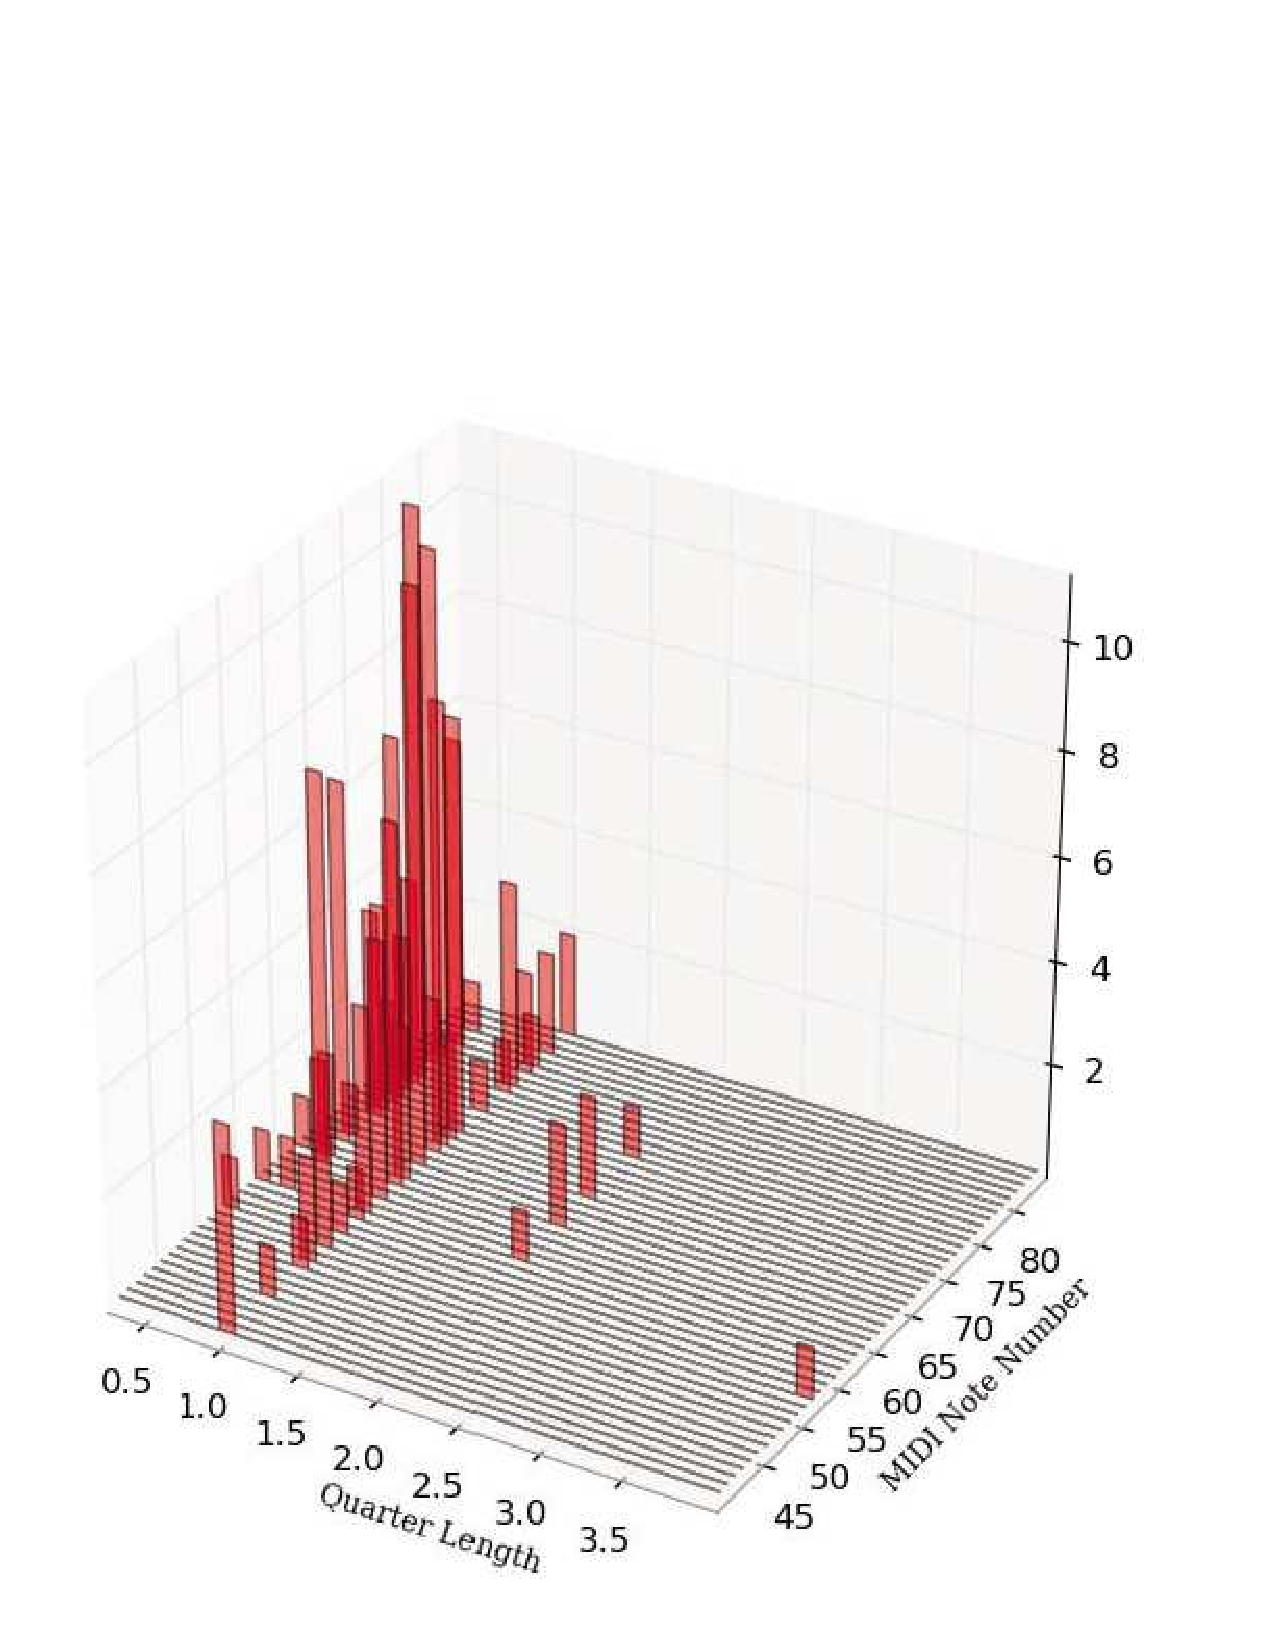
\includegraphics[width=0.8\textwidth, clip=true, trim = 15mm 10mm 20mm 70mm]{img/plot.pdf}
  \caption{Note Distribution by pitch and duration}
  \label{fig:note_distribution}
\end{figure}

The graph plots three features: pitch, duration of notes, and how frequently these pitches and
durations are used. It can be seen that pitches follow a type of bell-curve distribution, with few
high notes, few low notes, and many notes toward the middle of the register.  This line of inquiry
may reveal characteristics that are not easy to figure out, for instance, that a composer may be
following a certain trend.

\section{Summary}

With the \ac{DSL} \abcdt{} there is a considerable simplification of the process of creating an
\abcpt{} considering the following features:

\begin{itemize}
  \item It's not necessary to specify what doesn't need to be transformed (default functions);
  \item A transformation specification is rule-based which facilitates its writing;
  \item There's a set of rich \actuators{} which allows to precisely select a specific point to
  transform.
\end{itemize}

Using a structured processing of \abc{} allows an \abcpt{} to be described in an effective way.

Using Perl as the language embedded into \abcdt{} provides a rich environment to allow easy
processing of text. Furthermore, through the use of data structures, like hashes, the user has
bigger expressive power to specify transformations.\\

The next chapter presents some \abcpt{}s created using \abcdt{}.


  % What have I found? What does it mean?
  \chapter{ABC::DT by example}
  \label{chap:abc_dt_by_example}
  This chapter presents examples of \abcpt{}s created using \abcdt{}, thus demonstrating how easily a
(simple) tool or some occasional processing can be done. Some of the tools presented are an
extension of those presented in the article~\cite{Azevedo2013} submitted and accepted to
\emph{SLATE'13}'s conference.

The tools presented here are merely a proof of concept of what can be done with \abcdt{}, therefore,
they only provide a limited number of features and can be further improved in the future. However,
as they are, some of them have already proven their worth, consult chapter
\ref{chap:test_eval}.

Every \abcpt{} created performs at least one traversal to an \abc{} \ac{IR} (through \dt{}). So, in
order to facilitate the \abcdtrules{} readability for each \dt{} call, a tabular format will be
used, in which each row describes a single \abcdtrule{}.

%TODO nas regras (tabelas) por codigo perl mais bonito (fancy verbatim) ou letra mais pequena
%todo SE TIVER tempo por attach (midi)

\section{Paste ABC}
This tool, as the \unix{} \emph{paste}, merges voices parallel to each other in the time
perspective. In other words, each individual voice will start at the beginning of the resulting
score.

Some decisions were made regarding what should be done with some information present in each tune.
This ensured that the resulting tune was consistent with each individual tune:

\begin{enumerate}
  \item The resulting tune's header derives from the first tune which has an actual tune written, in
  other words, at least one \emph{note}.
  \item The \context{} is updated every time a change is detected during the tune's traversal. It is
  a local data structure that comprises the \emph{current voice} and its \emph{key}, \emph{meter},
  \emph{length}, \emph{tempo} and \emph{number of measures}.
  \item Any \context{} change detected, like the \emph{key} or the \emph{meter}, is written to the
  resulting tune only if it is different from the current \context{}.
  \item In the resulting tune, any voice that has fewer measures than the longest one is appended
  with the necessary \measurerests{} to match the longest.
\end{enumerate}

\subsection*{Algorithm}

\pasteabc{}'s algorithm is divided in three stages: \textbf{1)} retrieving the header for the
resulting tune, \textbf{2)} pasting the tunes and \textbf{3)} appending any necessary
\measurerests{}. In the end, the output generated is printed to the output.

An algorithmic description is made in algorithm \ref{alg:pasteabc}.

\begin{enumerate}
\item As mentioned before, the resulting tune's header comes from the first tune with at least
one \emph{note} written.

This stage follows a simple algorithm where each tune is processed by \dt{} in the order they are
passed in. As soon as a tune with a \emph{note} written is found, it stops and returns that tune's
header. During the tune's traversal, the \context{} is updated. It will be used in the final stage
where a post processing is done to guarantee the resulting tune's validity.

The set of \abcdtrules{} to be passed to \dt{} consists in applying a blank transformation to every
\abcelement{} with state \intune{} or \inline{} (consult section \ref{sec:abcdt_rules} for more
information on state), activating a flag when a \emph{note} is found to stop processing further
tunes and, finally, recording the \context{}. See table \ref{tab:paste_fst_stg_rules} for a
description of the \abcdtrules{}.

\begin{center}
  \begin{table}[h]
    \begin{tabular}{|p{2.25cm}|p{7.25cm}|p{5cm}|}
      \hline
      Actuator & Transformation (Perl) & Notes\\
      \hline
      \hline
      \intune{} & q\{\}; &
      \\
      \hline

      \hline
      \inline{} & q\{\}; &
      \\
      \hline

      \hline
      \emph{note} & \$has\_tune = 1; q\{\}; &
      \\
      \hline

      \hline
      \inheader{}::\emph{M:} & update\_context(\{meter => 1\}); toabc(); & \emph{update\_context} is
      a local function that updates, in this rule's case, the \context{}'s meter. \toabc{} is called
      in the end so that the actual \abcelement{} is printed instead of the returning value from the
      previous statement.
      \\
      \hline

      \hline
      \inheader{}::\emph{L:} & update\_context(\{length => 1\}); toabc(); &
      \\
      \hline

      \hline
      \inheader{}::\emph{K:} & update\_context(\{key => 1\}); toabc(); &
      \\
      \hline

      \hline
      \inheader{}::\emph{Q:} & update\_context(\{tempo => 1\}); toabc(); &
      \\
      \hline
    \end{tabular}
    \caption{\abcdtrules{} for \pasteabc{}'s first stage}
    \label{tab:paste_fst_stg_rules}
  \end{table}
\end{center}

\item This stage's consists in processing each tune with \dt{} and concatenating each individual
result. This is the actual pasting where each tune's original \abc{} is returned except for the
following parts.

The header from each tune is not printed since it has already been retrieved in the previous stage.

abcMIDI commands \emph{\%\%staves} and \emph{\%\%score} are not printed as well, since each voice's
positioning on the resulting score may differ from the original one.

The \context{} is also being recorded each time one of its constituents is found, which enables the
possibility of not printing the context change if it is the same as the current one. This makes the
resulting tune cleaner without useless duplications. See table \ref{tab:paste_snd_stg_rules}.

\begin{center}
  \begin{table}[h]
    \begin{tabular}{|p{2.5cm}|p{4.75cm}|p{8cm}|}
      \hline
      Actuator & Transformation (Perl) & Notes\\
      \hline
      \hline
      \emph{in\_global::info} & q\{\}; &
      \\
      \hline

      \hline
      \emph{in\_header::info} & q\{\}; &
      \\
      \hline

      \hline
      \emph{staves} & q\{\}; &
      \\
      \hline

      \hline
      \emph{score} & q\{\}; &
      \\
      \hline

      \hline
      \emph{bar} & update\_measure\_count(); toabc(); & \emph{update\_measure\_count} is a local
      function that increments the measure count for the current voice.
      \\
      \hline

      \hline
      \emph{V:} & print\_voice(); & Local function that prints the voice element if it is different
      from the current voice. Also, if this voice has been previously defined, then the short form
      of the voice's \abcelement{} is printed. \context{}'s voice is updated.
      \\
      \hline

      \hline
      \emph{M:} & print\_meter(); & Local function that prints the meter element if it is different
      from the current meter. \context{}'s meter is updated.
      \\
      \hline

      \hline
      \emph{L:} & print\_length(); & Same as the previous rule but applied to the length element.
      \\
      \hline

      \hline
      \emph{K:} & print\_key(); & Same as the previous rule but applied to the key element.
      \\
      \hline

      \hline
      \emph{Q:} & print\_tempo(); & Same as the previous rule but applied to the tempo element.
      \\
      \hline

    \end{tabular}
    \caption{\abcdtrules{} for \pasteabc{}'s second stage}
    \label{tab:paste_snd_stg_rules}
  \end{table}
\end{center}

\item The final step consists in verifying if there is any voice with fewer measures than the voice
with the biggest number of measures. If there is such a voice then a \measurerest{} with length
equal to the missing measures is appended after that voice. This is possible because, in step
\textbf{2)}, the number of measures for each voice was being recorded.
\end{enumerate}

\begin{algorithm}[h]
  \KwIn{abc\_tunes}
  \ForAll{$ tune \in abc\_tunes $}{
    $header \gets dt(tune,$ rules from table \ref{tab:paste_fst_stg_rules}$)$ \hfill //1)\\
  }
  \ForAll{$ tune \in abc\_tunes $}{
    $res \gets res$ ++ $dt(tune,$ rules from table \ref{tab:paste_snd_stg_rules}$)$ \hfill //2)\\
  }
  $measures \gets add\_measures()$ \hfill //3)\\
  \Return{$header$ ++ $res$ ++ $measures$}
  \caption{\pasteabc{}'s algorithm}
  \label{alg:pasteabc}
\end{algorithm}

\subsection*{Usage}

Listing \ref{lst:pasteabcman} shows \pasteabc{}'s manual.\\

\lstinputlisting[caption={\pasteabc{}'s manual},label={lst:pasteabcman},captionpos=t,abovecaptionskip=-\medskipamount,float]{misc/paste_manual.tex}

Listing \ref{lst:paste_abc_by_example} shows a usage example for \pasteabc{}. It reads tunes
\textbf{101.abc} (listing \ref{lst:verbum_s1_p1}) and \textbf{103.abc} (listing
\ref{lst:verbum_s1_p3}) and its output is shown in listing \ref{lst:verbum_s1_p1_p3_pasted} along
with the corresponding score (figure \ref{fig:verbum_s1_p1_p3_score}).\\

\begin{lstlisting}[caption={\pasteabc{} by example},label={lst:paste_abc_by_example},captionpos=t,abovecaptionskip=-\medskipamount]
paste_abc 101.abc 103.abc
\end{lstlisting}

\lstinputlisting[caption={Verbum caro factum est: Section 1; Part 1 - Soprano},label={lst:verbum_s1_p1},captionpos=t,abovecaptionskip=-\medskipamount]{misc/verbum_s1_p1.tex}

\vspace{-0.25cm}
\begin{figure}[H]
  \begin{center}
    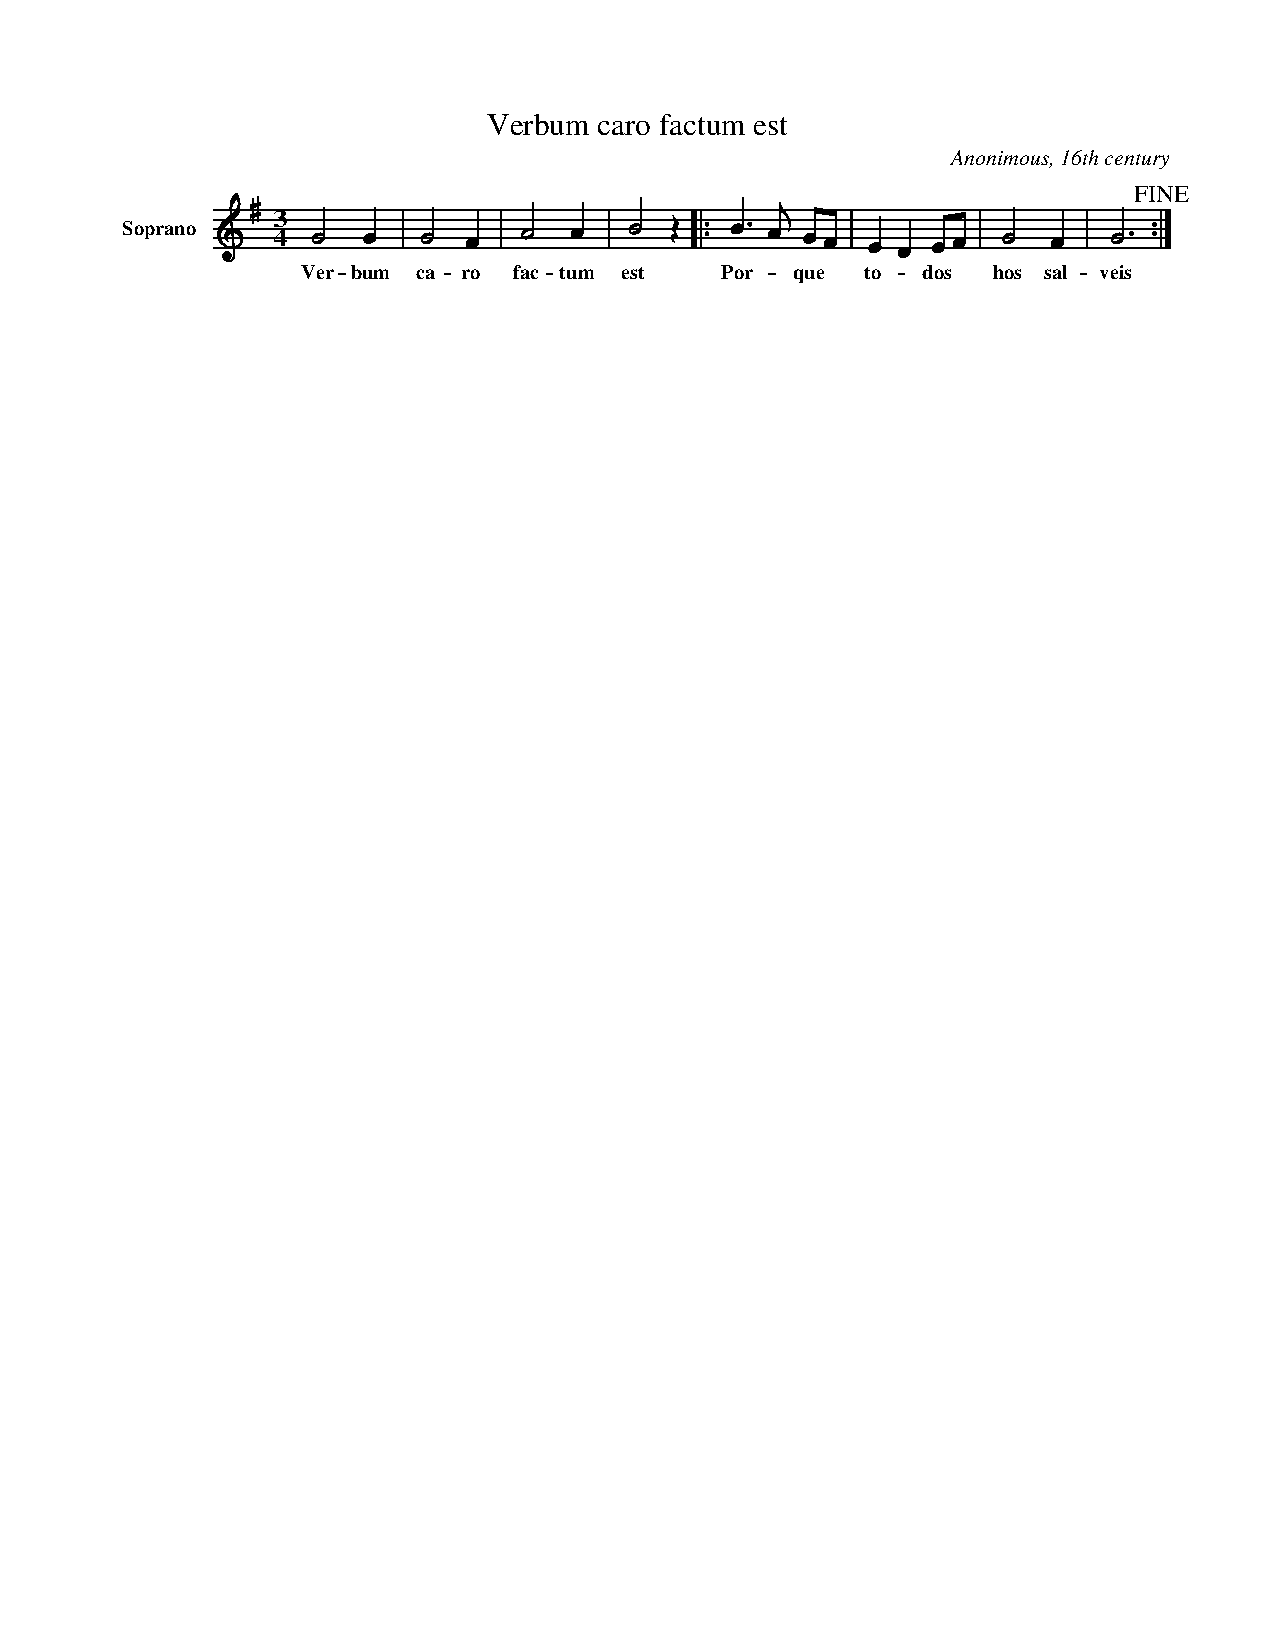
\includegraphics[width=0.8\textwidth, clip=true, trim = 0mm 230mm 0mm 17mm]{img/101.pdf}
    \caption{Verbum caro factum est: Section 1; Part 1 - Soprano (Score)}
    \label{fig:verbum_s1_p1_score}
  \end{center}
\end{figure}

\lstinputlisting[caption={Verbum caro factum est: Section 1; Part 3 - Tenor},label={lst:verbum_s1_p3},captionpos=t,abovecaptionskip=-\medskipamount]{misc/103.tex}

\vspace{-1.30cm}
\begin{figure}[h]
  \begin{center}
    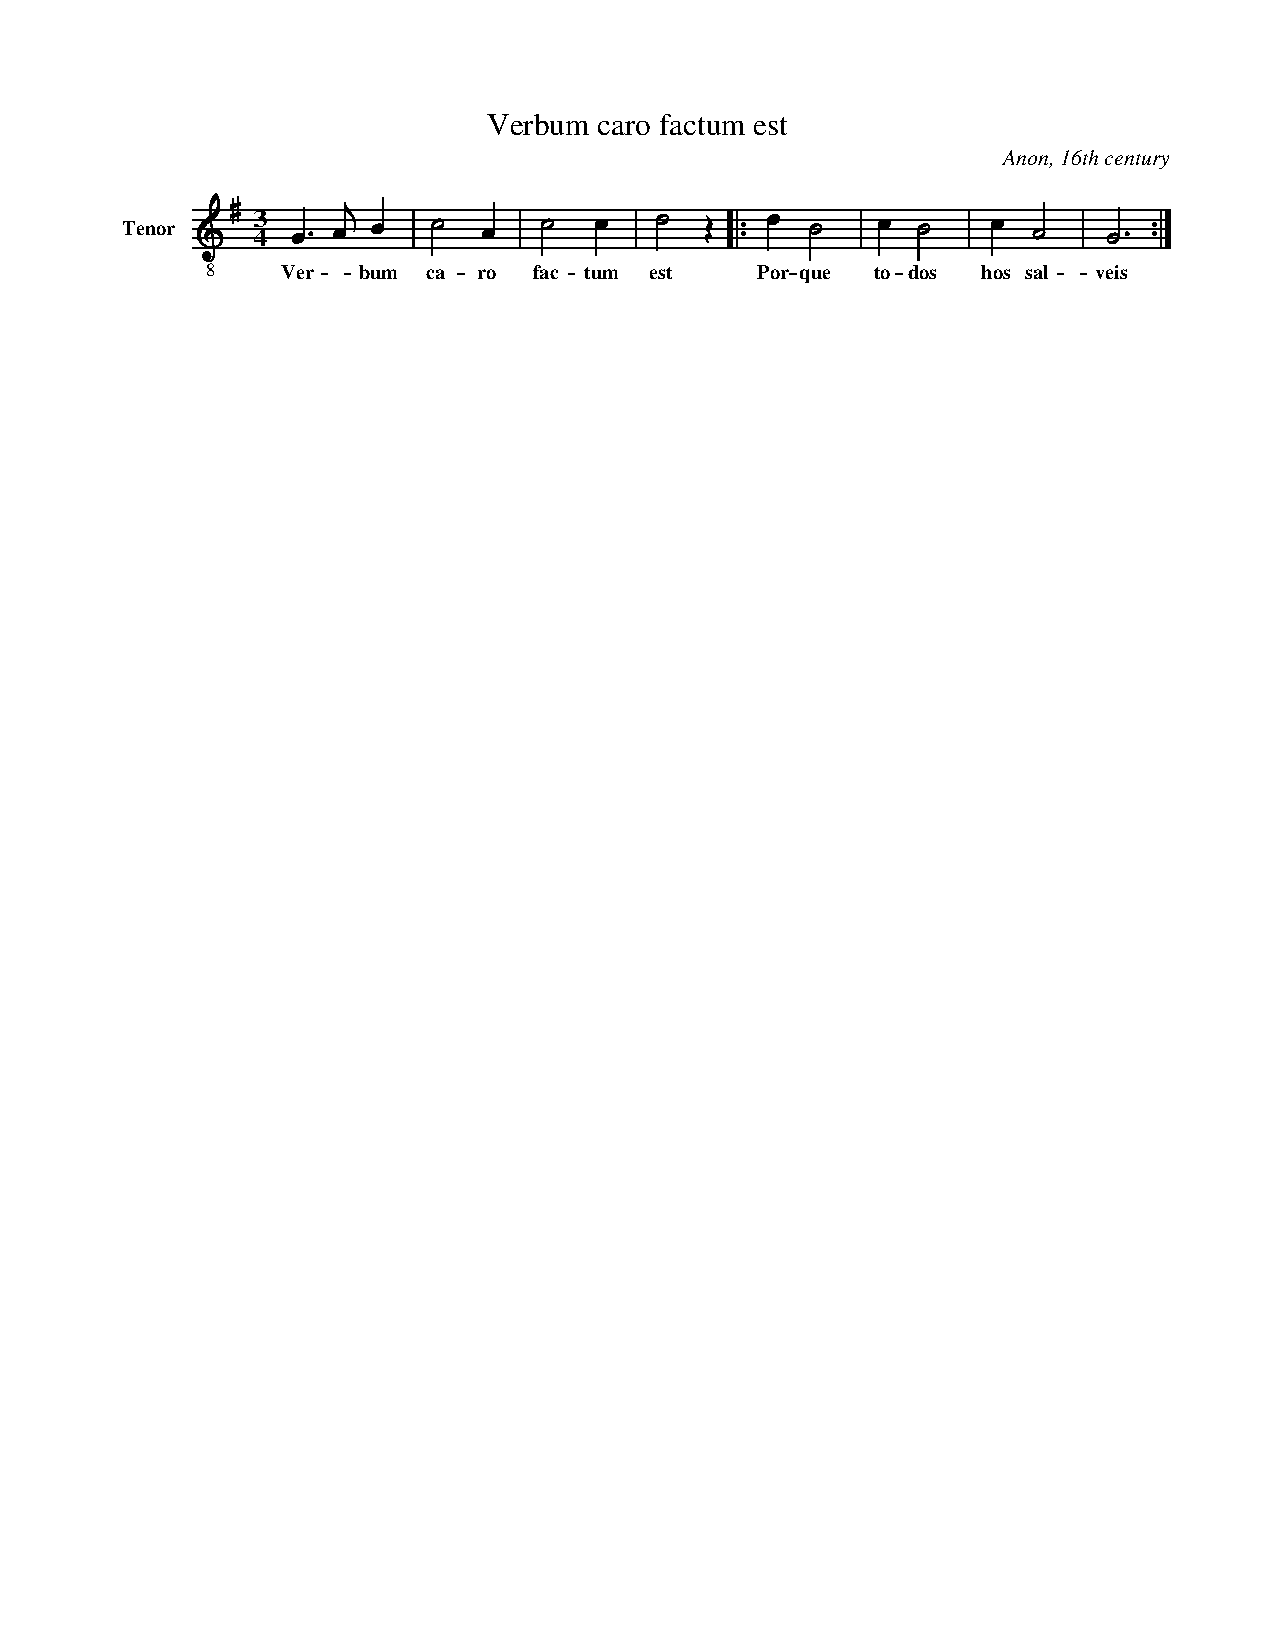
\includegraphics[width=0.8\textwidth, clip=true, trim = 15mm 231mm 17mm 0mm]{img/103.pdf}
    \caption{Verbum caro factum est: Section 1; Part 3 - Tenor (Score)}
  \end{center}
\end{figure}

\lstinputlisting[caption={Verbum caro factum est: Section 1; Part 1 \& 3},label={lst:verbum_s1_p1_p3_pasted},captionpos=t,abovecaptionskip=-\medskipamount]{misc/verbum_s1_p1_p3_pasted.tex}

\vspace{-1.30cm}
\begin{figure}[h]
  \begin{center}
    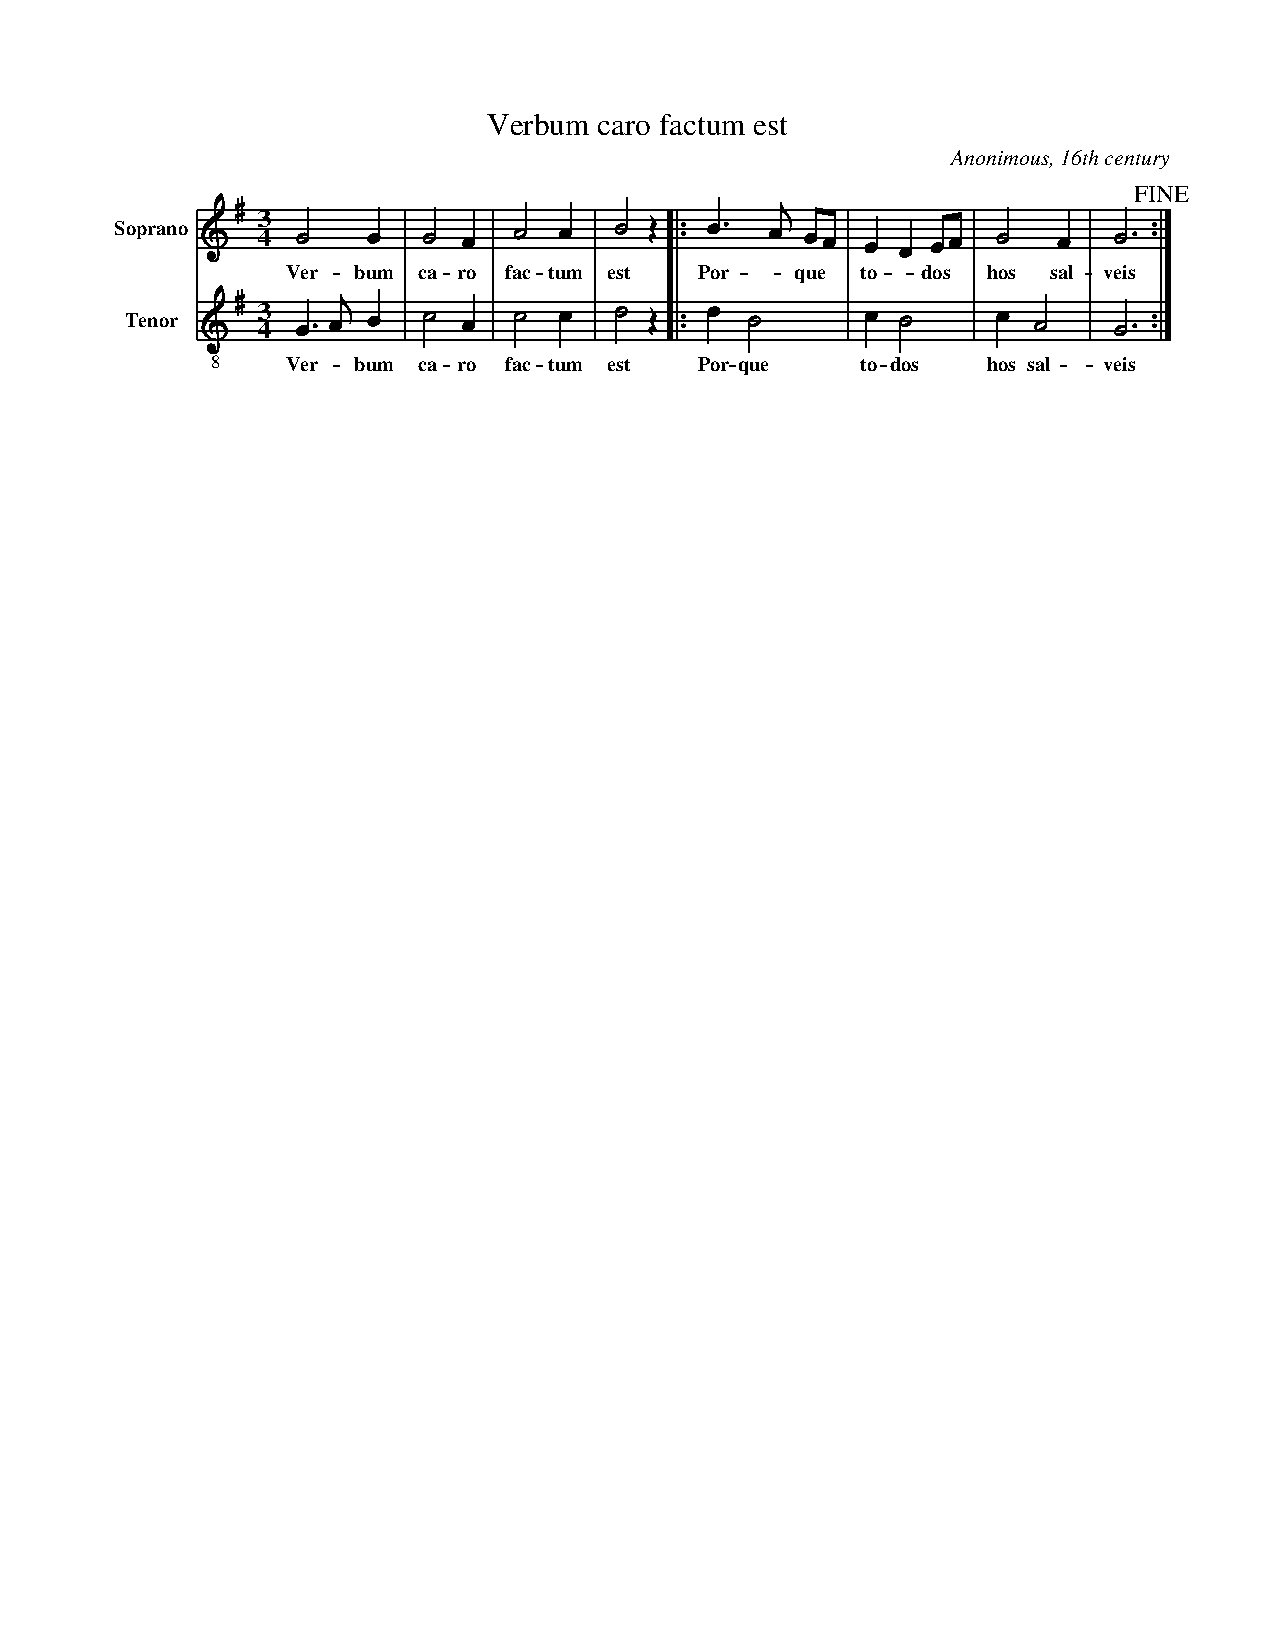
\includegraphics[width=0.8\textwidth, clip=true, trim = 15mm 210mm 15mm 0mm]{img/verbum_s1_p1_p3.pdf}
    \caption{Verbum caro factum est: Section 1; Part 1 \& 3 (Score)}
    \label{fig:verbum_s1_p1_p3_score}
  \end{center}
\end{figure}


\section{Cat ABC}
This tool is based on \unix{}'s \emph{cat}, as it consists in the concatenation of each tune one
after the other in the time perspective. In other words, any voice present in the second tune is
printed after the time offset corresponding to the end of the first tune, and so on.

Some design goals were established:

\begin{enumerate}
  \item The resulting tune's header derives from the first tune which has an actual tune written, in
  other words, at least one \emph{note}.
  \item The \context{} is updated every time a change is detected during the tune's traversal. It is
  a local data structure that comprises the \emph{current voice} and its \emph{key}, \emph{meter},
  \emph{length} and \emph{tempo}. The \emph{number of measures} per voice is recorded separately for
  each tune.
  \item Any \context{} change detected, like the \emph{key} or the \emph{meter}, is written to the
  resulting tune only if it is different from the current \context{}.
  \item For each tune, before appending it to the resulting tune, a verification for missing voices
  is made in the current tune and all prior to that. This way, \measurerests{} can be appended to any
  missing voice in order to ensure that the voice starts at the correct time offset.
  \item In the resulting tune, any voice that has fewer measures than the longest one is appended
  with the necessary \measurerests{} to match the longest.
\end{enumerate}

\subsection*{Algorithm}

\catabc{}'s algorithm is similar to \pasteabc{}'s except that after processing an \abc{} tune with
\dt{}, \measurerests{} may be appended to some voices before and after the actual tune is written.
Since all voices in an \abc{} file are written after the time offset corresponding to the end of the
previous \abc{} file, there may be music missing for some voices from one file to the other, thus
the need for \measurerests{} to fill those "holes".

So the algorithm has the following stages: \textbf{1)} retrieving the header for the resulting tune,
\textbf{2)} printing each tune and any necessary \measurerests{}. In the end, the output generated
is printed to the output.

An algorithmic description is made in algorithm \ref{alg:catabc}.

\begin{enumerate}
  \item The resulting tune's header comes from the first tune with at least one \emph{note} written.

  This stage does exactly the same as \pasteabc{}'s first stage.

  \item For each tune:

  \begin{enumerate}
    \item Applies \dt{} to the current tune;
    \item Appends \measurerests{} to every voice that is present in previous tunes and not in the current one;
    \item Appends \measurerests{} to every voice presented for the first time;
    \item Appends \dt{}'s output, which is the actual tune;
    \item Appends any necessary \measurerests{} to the processed tune (same as stage \textbf{3)} in
    \pasteabc{}'s main algorithm);
  \end{enumerate}

  \begin{program}
    When concatenating tune \emph{A} with tune \emph{B} and tune \emph{B} is being processed, step
    \textbf{b)} appends the \measurerests{} illustrated by the letter \emph{P1} and step \textbf{c)}
    appends the \measurerests{} illustrated by the letter \emph{P2}.

    % \vspace{-1.30cm}
    \begin{center}
      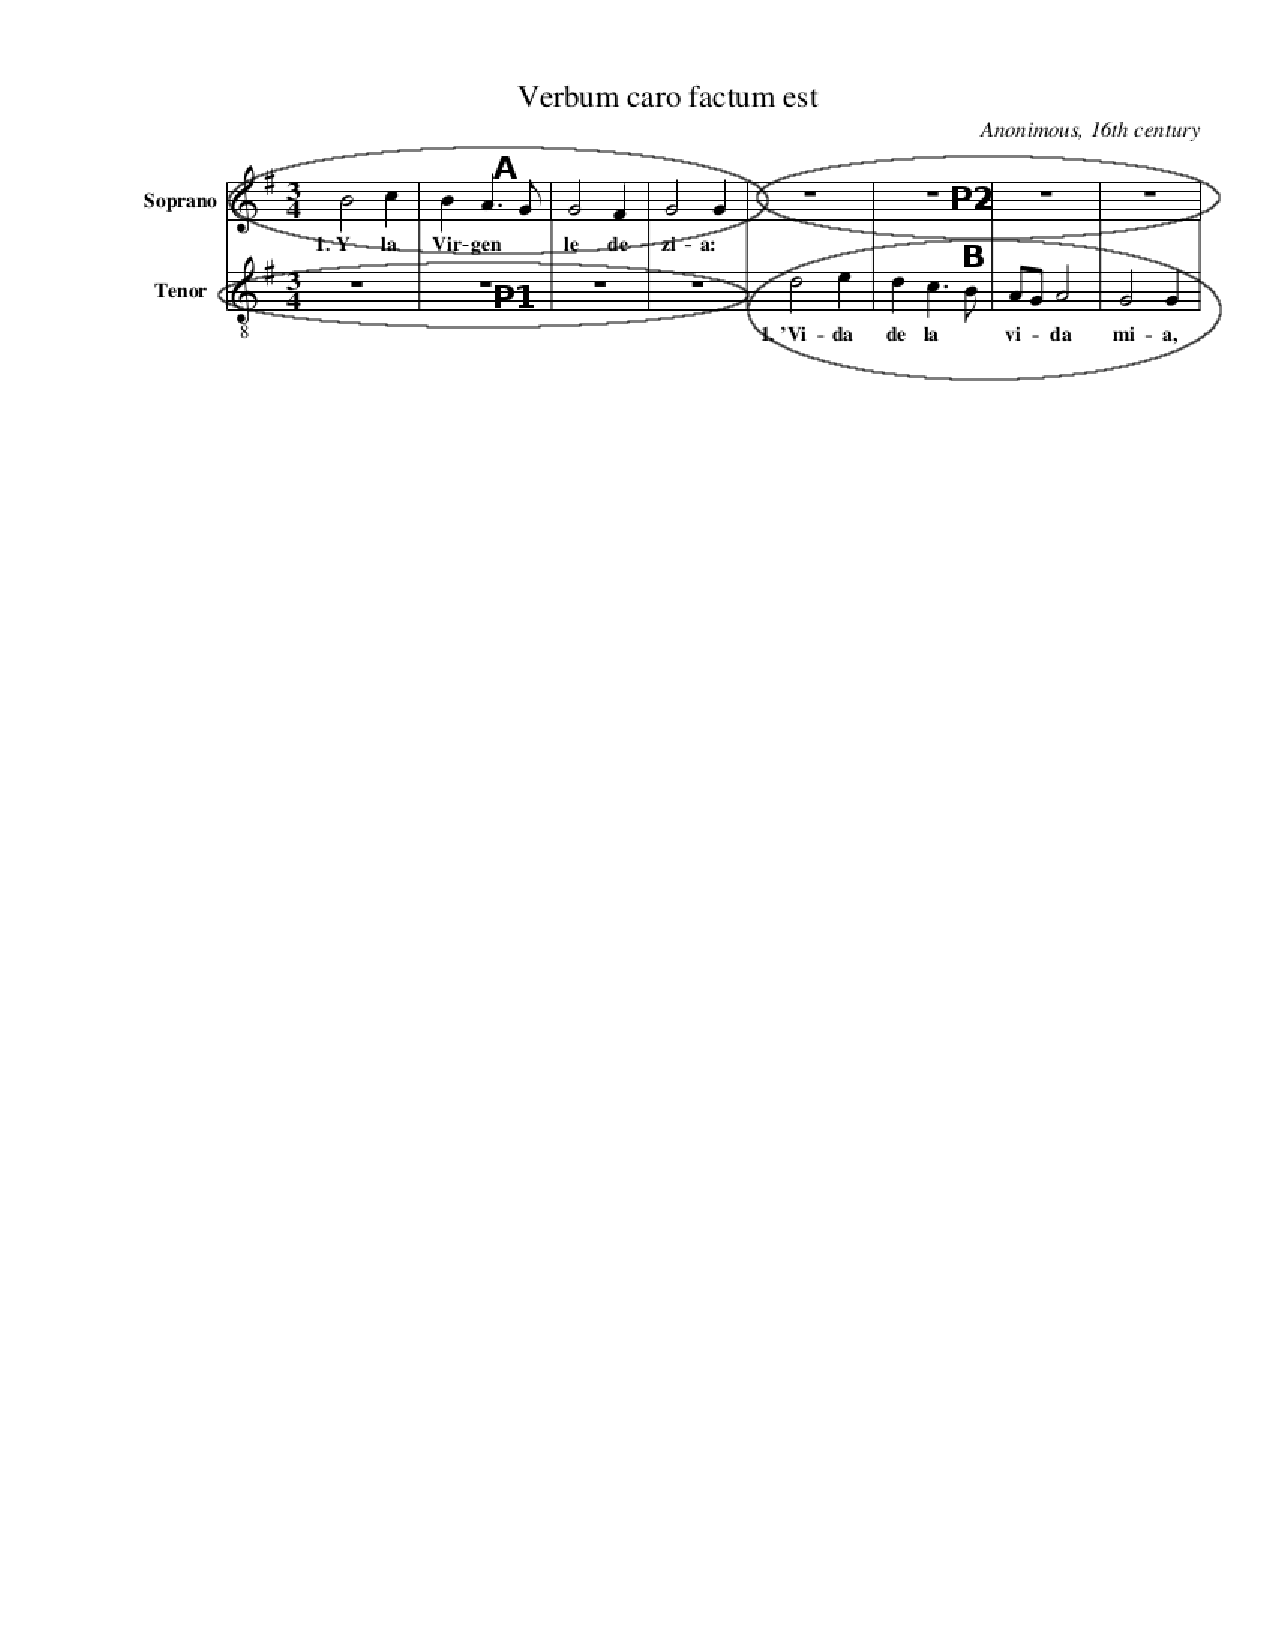
\includegraphics[width=0.8\textwidth, clip=true, trim = 15mm 213mm 0mm 10mm]{img/verbum_measures.pdf}
    \end{center}

    \caption{Appending necessary \measurerests{}}
  \end{program}

  Each individual result is concatenated into the resulting tune.\\

  The set of \abcdtrules{} used in this stage is the same as in \pasteabc{}'s second stage. However,
  \catabc{} provides two more options for concatenating tunes: inserting a number of \measurerests{}
  at the beginning of each tune (option \emph{-d}) and repeating each tune a number of times (option
  \emph{-r}).

  To implement the first option, some modifications were made to the set of \abcdtrules{}:

  \begin{itemize}
    \item The default transformation for each \abcelement{} is not \toabc{}, but instead a local
    function that, once for each voice, inserts a \measurerest{} with the request length before the
    element itself and also updates the \context{}'s measure count for that voice.
    \item The \context{}'s measure count update is made when a \emph{bar} or a \emph{mrest} is
    found.
  \end{itemize}

  Those modifications are described in table \ref{tab:cat_snd_stg_rules}.

  \begin{center}
    \begin{table}[h]
      \begin{tabular}{|p{2.5cm}|p{4.75cm}|p{8cm}|}
        \hline
        Actuator & Transformation (Perl) & Notes\\
        \hline
        \hline
        \emph{bar} & update\_measure\_count(1); insert\_canon\_delta(); &
        \emph{update\_measure\_count} is a local function that increments, in this case by 1, the
        \context{}'s measure count for the current voice. \emph{insert\_canon\_delta} is a local
        function that inserts a \measurerest{} before the element itself, once for each voice.
        \\
        \hline

        \hline
        \emph{mrest} & update\_measure\_count( \$sym->\{info\}->\{len\} - 1 );
        insert\_canon\_delta(); &
        \emph{\$sym} is the \abcelement{} currently being processed, a \measurerest{}.
        \emph{\$sym->\{info\}->\{len\}} is the number of measures in rest.
        \\
        \hline

        \hline
        \emph{-default} & insert\_canon\_delta(); &
        \\
        \hline
      \end{tabular}
      \caption{\abcdtrules{} for \catabc{}'s second stage}
      \label{tab:cat_snd_stg_rules}
    \end{table}
  \end{center}

  The second option is obtained by simply repeating steps \textbf{a} to \textbf{e} a requested
  number of times.
\end{enumerate}

\begin{algorithm}[h]
  \KwIn{abc\_tunes}
  \ForAll{$ tune \in abc\_tunes $}{
    $header \gets dt(tune,$ rules from table \ref{tab:paste_fst_stg_rules}$)$ \hfill //1)\\
  }
  \ForAll{$ tune \in abc\_tunes $}{
    \For{$ 0 .. $ value of \emph{-r} option }{
      $c\_tune \gets dt(tune,$ rules from tables \ref{tab:paste_snd_stg_rules} and \ref{tab:cat_snd_stg_rules}$)$ \hfill //2-a)\\
      $res \gets res$ ++ $add\_measures\_to\_missing\_voices()$ \hfill //2-b)\\
      $res \gets res$ ++ $add\_measures\_to\_new\_voices()$ \hfill //2-c)\\
      $res \gets res$ ++ $c\_tune$ \hfill //2-d)\\
      $res \gets res$ ++ $add\_measures()$ \hfill //2-e)\\
    }
  }
  \Return{$header$ ++ $res$}
  \caption{\catabc{}'s algorithm}
  \label{alg:catabc}
\end{algorithm}

\subsection*{Usage}

Listing \ref{lst:catabcman} shows \catabc{}'s manual.\\

\lstinputlisting[caption={\catabc{}'s manual},label={lst:catabcman},captionpos=t,abovecaptionskip=-\medskipamount]{misc/cat_manual.tex}

Listing \ref{lst:cat_abc_by_example} shows a usage example for \catabc{}. It reads tunes
\textbf{201.abc} (listing \ref{lst:verbum_s2_p1}) and \textbf{303.abc} (listing
\ref{lst:verbum_s3_p3}) and the output is shown in listing \ref{lst:verbum_s2_p1_s3_p3_cated} with
its respective score (figure \ref{fig:verbum_s2_p1_s3_p3}).\\

\begin{lstlisting}[caption={\catabc{} by example},label={lst:cat_abc_by_example},captionpos=t,abovecaptionskip=-\medskipamount]
cat_abc 201.abc 303.abc
\end{lstlisting}

\lstinputlisting[caption={Verbum caro factum est: Section 2; Part 1 - Soprano},label={lst:verbum_s2_p1},captionpos=t,abovecaptionskip=-\medskipamount]{misc/201.tex}

\vspace{-1.30cm}
\begin{figure}[h]
  \begin{center}
    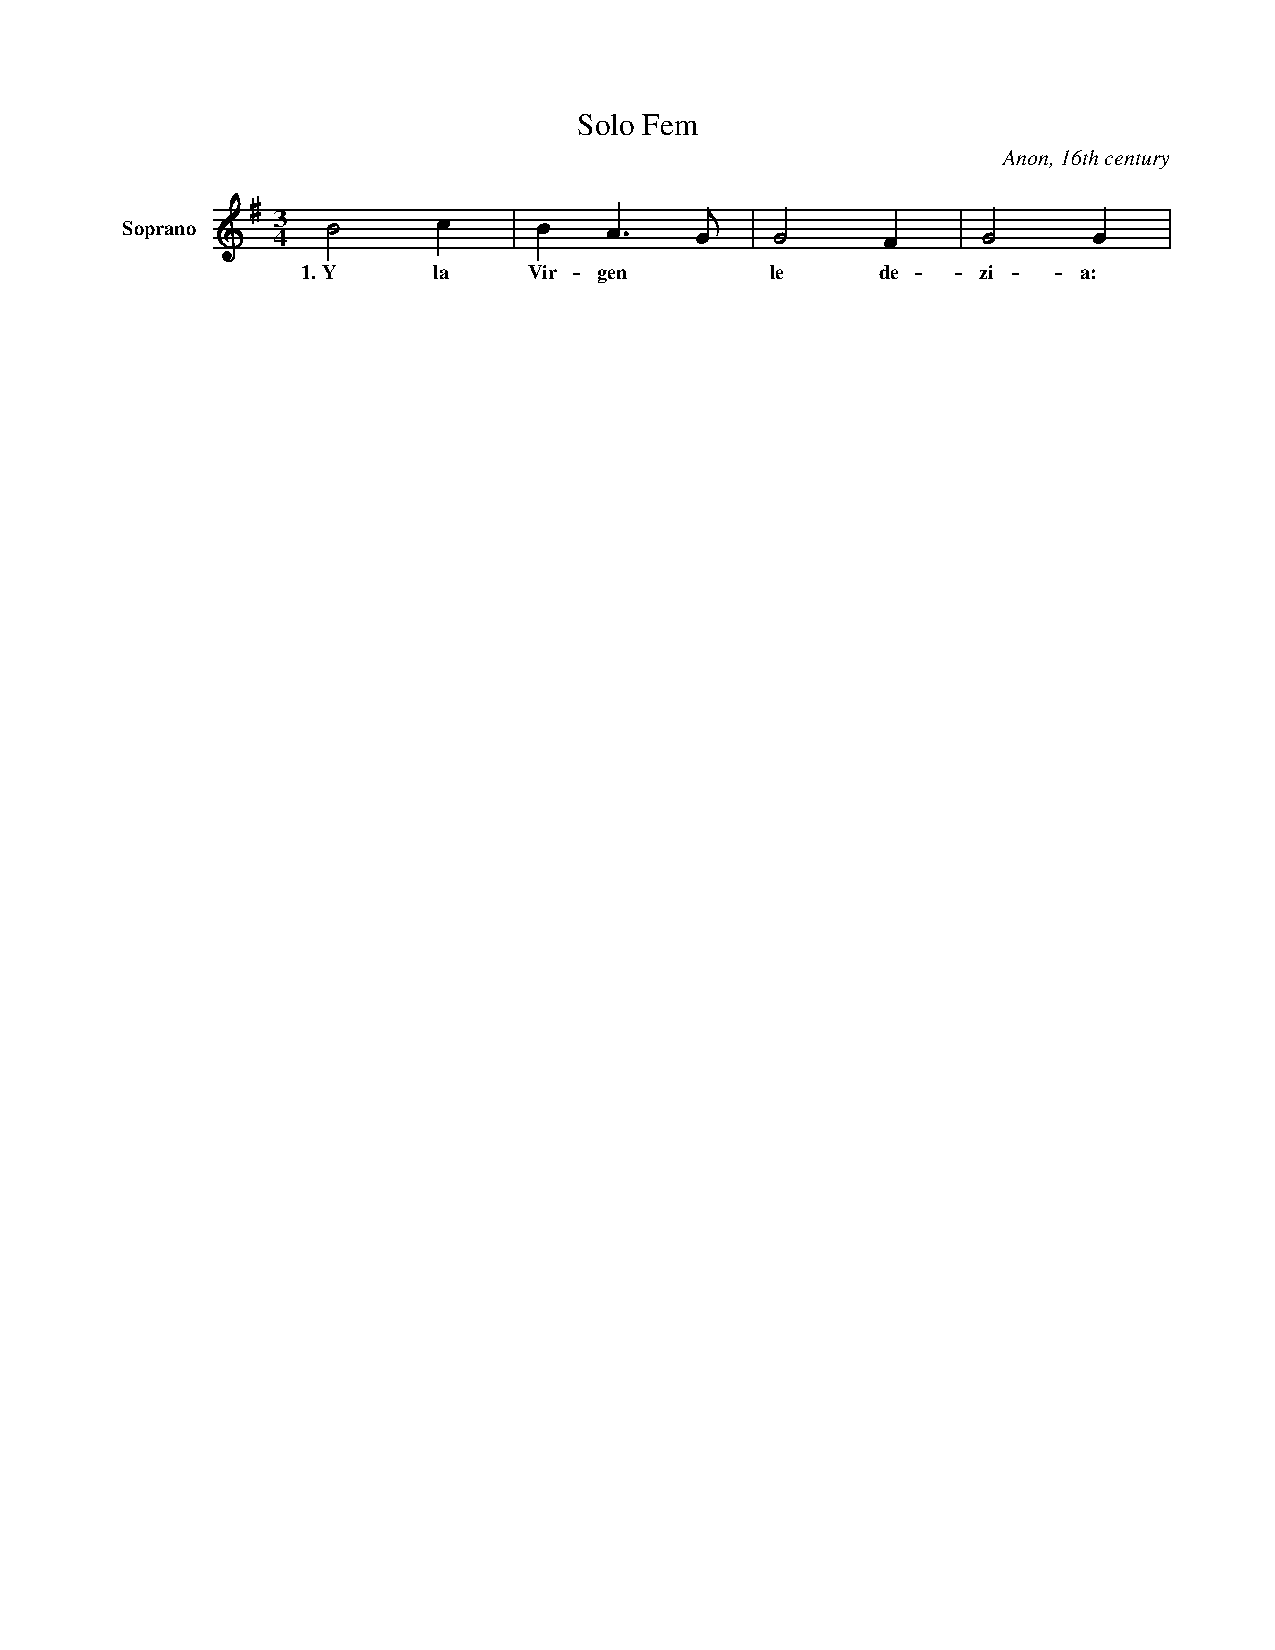
\includegraphics[width=0.8\textwidth, clip=true, trim = 15mm 231mm 0mm 0mm]{img/201.pdf}
    \caption{Verbum caro factum est: Section 2; Part 1 - Soprano (Score)}
  \end{center}
\end{figure}

\lstinputlisting[caption={Verbum caro factum est: Section 3; Part 3 - Tenor},label={lst:verbum_s3_p3},captionpos=t,abovecaptionskip=-\medskipamount]{misc/303.tex}

% \vspace{-1.30cm}
\begin{figure}[H]
  \begin{center}
    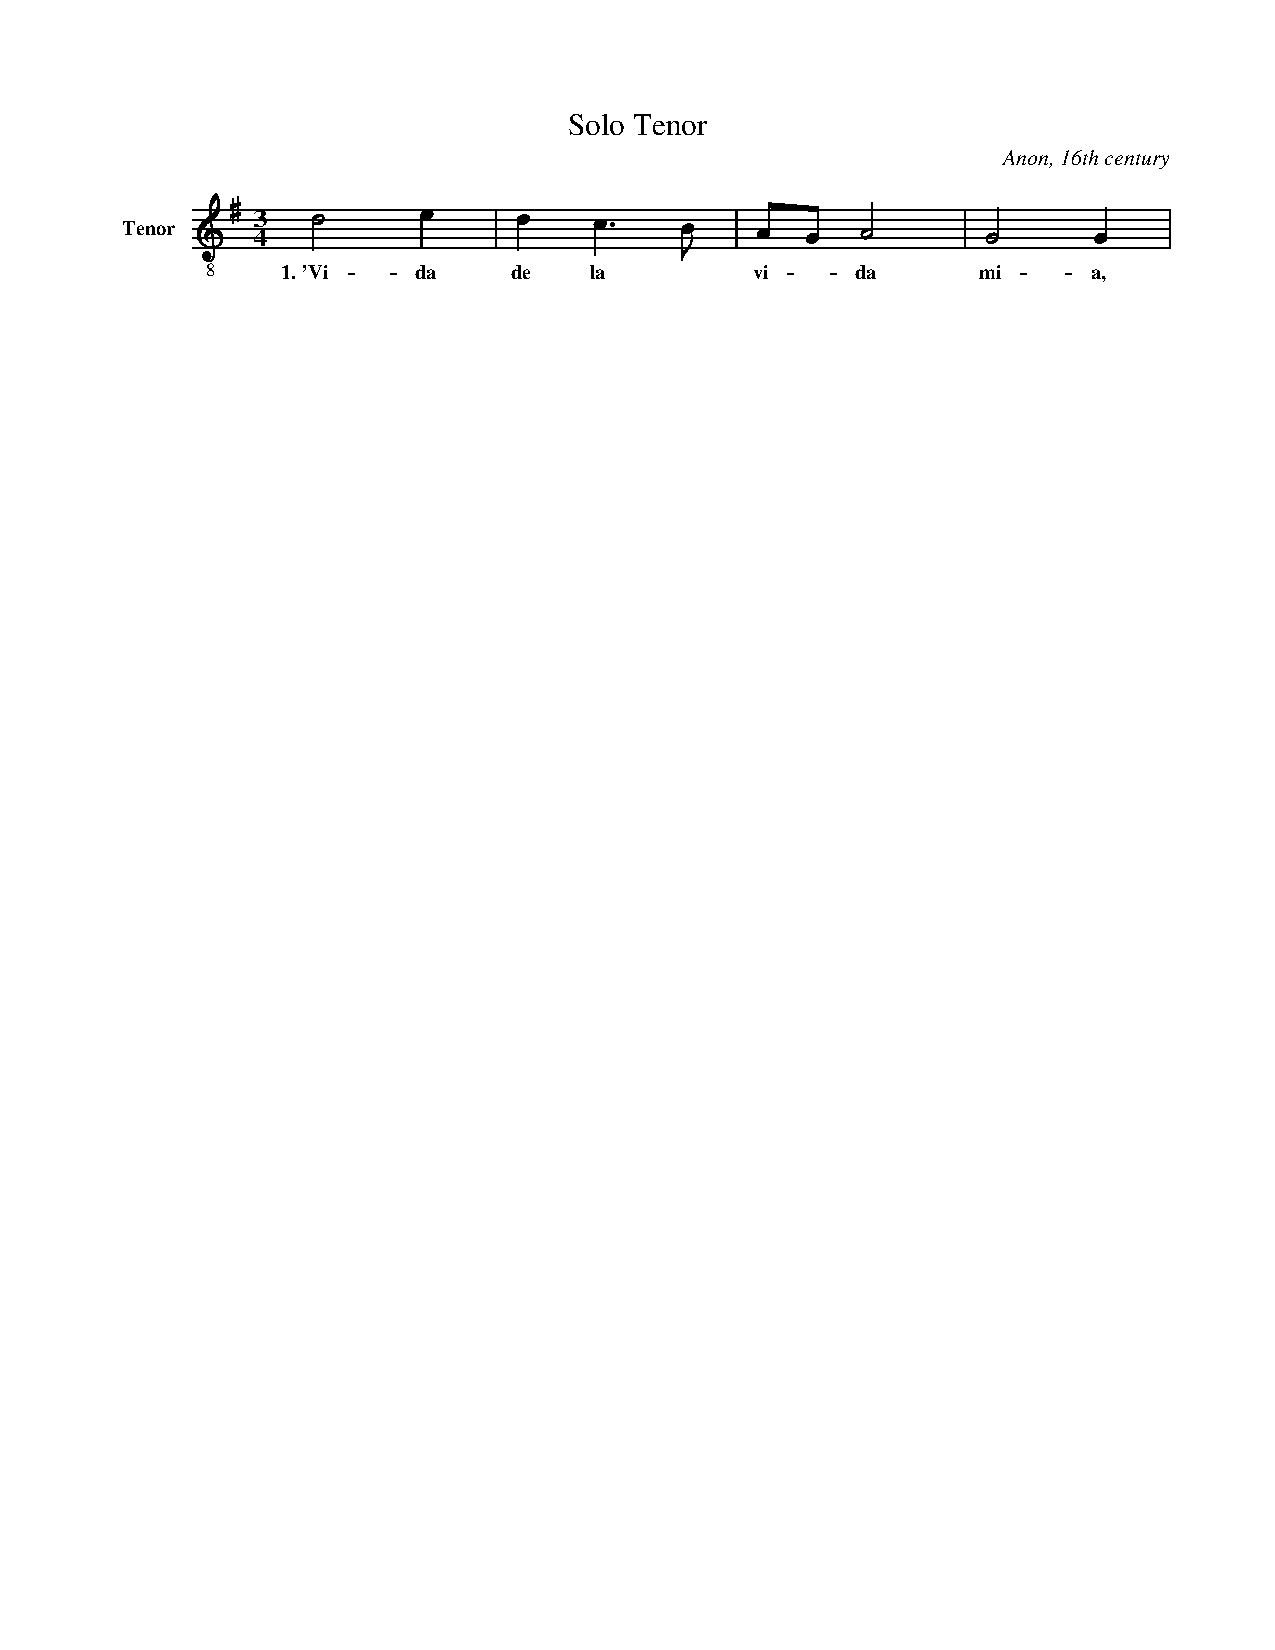
\includegraphics[width=0.8\textwidth, clip=true, trim = 15mm 231mm 0mm 0mm]{img/303.pdf}
    \caption{Verbum caro factum est: Section 3; Part 3 - Tenor (Score)}
  \end{center}
\end{figure}

\lstinputlisting[caption={Verbum caro factum est: Section 2; Part 1 \& Section 3: Part 3},label={lst:verbum_s2_p1_s3_p3_cated},captionpos=t,abovecaptionskip=-\medskipamount]{misc/verbum_s2_p1_s3_p3_cated.tex}

\vspace{-1.50cm}
\begin{figure}[H]
  \begin{center}
    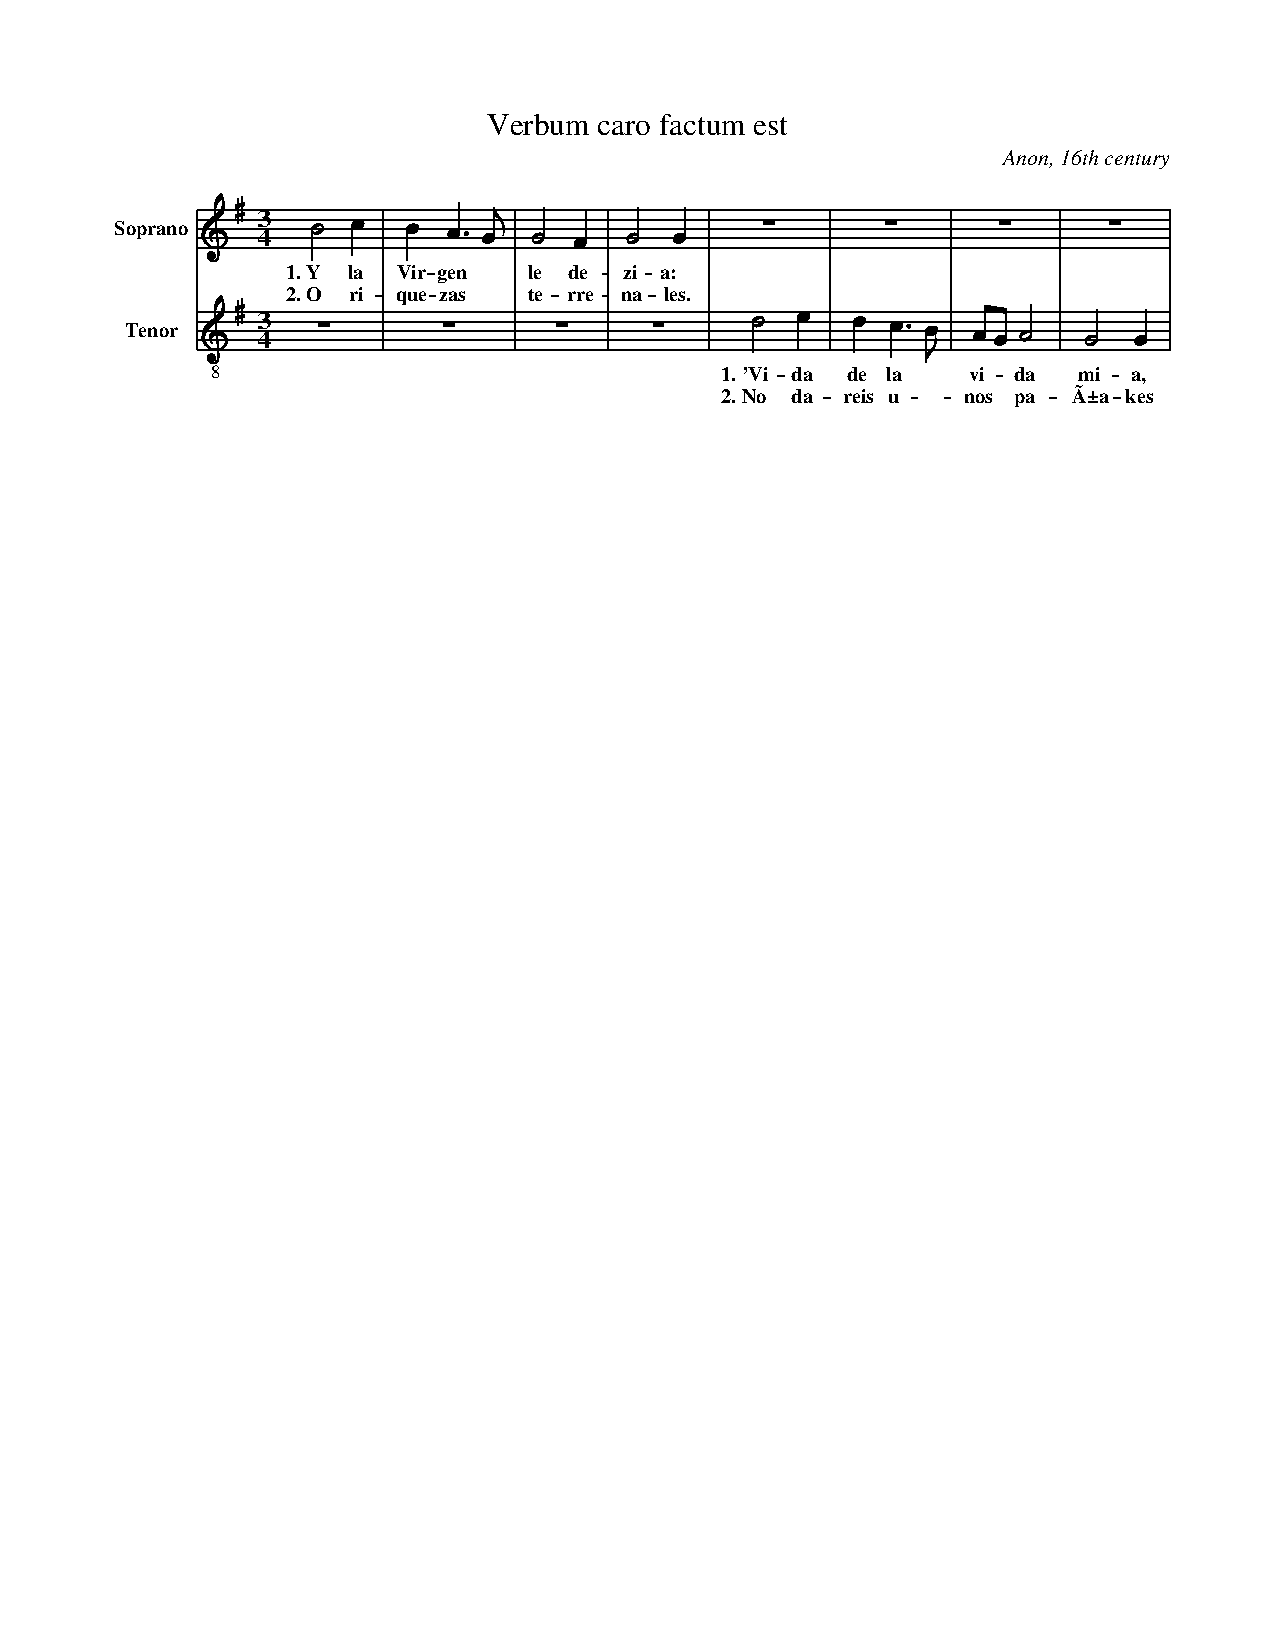
\includegraphics[width=0.8\textwidth, clip=true, trim = 18mm 210mm 16mm 0mm]{img/verbum_s2_p1_s3_p3.pdf}
    \caption{Verbum caro factum est: Section 2; Part 1 \& Section 3: Part 3 (Score)}
    \label{fig:verbum_s2_p1_s3_p3}
  \end{center}
\end{figure}


\section{Learning ABC}
When there is a multi-voice score, like a four part choir, it is important to, for instance, the
Soprano to be able to study her part individually. Sometimes there's the need to hear all the other
parts except hers, so that she may know what the rest is going to sound. Other times the opposite is
what is needed.

The \learningabc{} tool generates two \abc{} scores whose goal is to help musicians in individual
rehearsal of multi-voice music for studying purposes. One reduces the volume of a particular voice
and the other increases the volume of a particular voice and reduces the volume of the remaining
voices.

\subsection*{Algorithm}

\learningabc{}'s algorithm consists of 3 stages that are applied to each tune.

An algorithmic description is made in algorithm \ref{alg:learningabc}.\\

For each tune:
\begin{enumerate}
  \item \textbf{Retrieve voice data}

  In this stage, the tune is processed by \dt{}, in which each voice's name, channel and program
  (instrument) are stored to be used in the following stages.

  The set of \abcdtrules{} is shown in table \ref{tab:learning_abc_fst_stage}.

  \begin{center}
    \begin{table}[h]
      \begin{tabular}{|p{3cm}|p{5cm}|p{7.5cm}|}
        \hline
        Actuator & Transformation (Perl) & Notes\\
        \hline
        \hline
        \emph{V:} & store\_channel\_and\_name(); & Local function that stores each voice's channel
        and name.
        \\
        \hline

        \hline
        \emph{MIDI::program} & store\_program(); & Local function that stores each voice's program.
        \\
        \hline
      \end{tabular}
      \caption{\abcdtrules{} for \learningabc{}'s first stage}
      \label{tab:learning_abc_fst_stage}
    \end{table}
  \end{center}

  \item \textbf{All but one}

  In \abc{}, it is possible to add commands to control audio properties through the use of \midi{}
  directives (\emph{\%\%MIDI}, followed by different parameters) that \abctomidi{} recognizes.

  In this stage, the tune is processed by \dt{}, in which a \midi{} directive to reduce the volume
  of the voice is inserted. To be more precise, a change-volume \midi{} directive (\emph{\%\%MIDI
  control 7 NewVolume}, where \emph{NewVolume} is a number between (0-127)- is appended after the
  voice definition.

  In the end, the processed tune is written to a new \abc{} file.

  The set of \abcdtrules{} is shown in table \ref{tab:learning_abc_snd_stage}.

  \begin{center}
    \begin{table}[h]
      \begin{tabular}{|p{2.25cm}|p{6.75cm}|p{6.5cm}|}
        \hline
        Actuator & Transformation (Perl) & Notes\\
        \hline
        \hline
        \emph{V:\$req\_voice} & toabc() . "\%\%MIDI control 7 \$min\_volume\textbackslash{}n"); &
        \emph{\$req\_voice} keeps the voice requested when calling \learningabc{}.
        \\
        \hline
      \end{tabular}
      \caption{\abcdtrules{} for \learningabc{}'s second stage}
      \label{tab:learning_abc_snd_stage}
    \end{table}
  \end{center}

  \item \textbf{Just one}

  In this stage, the tune is processed by \dt{}, in which, for each voice, three \midi{} directives
  are inserted after the \emph{X:} statement. The first is a select-channel directive
  (\emph{\%\%MIDI channel Channel}, where \emph{Channel} is a number between (1-16)), the second a
  select-program directive (\emph{\%\%MIDI program Channel Program}, where \emph{Program} is the
  instrument (0-127) for channel \emph{Channel}) and the third is a change-volume directive to
  reduce or increase the voice's volume. Furthermore, the select-channel directive is also appended
  to the voice statement so that \abctomidi{} can make the association between the voice and the
  channel when reproducing.

  In the end, the processed tune is written to a new \abc{} file.

  The set of \abcdtrules{} is shown in table \ref{tab:learning_abc_trd_stage}.

  \begin{center}
    \begin{table}[h]
      \begin{tabular}{|p{1.5cm}|p{7.5cm}|p{6.5cm}|}
        \hline
        Actuator & Transformation (Perl) & Notes\\
        \hline
        \hline
        \emph{X:} & set\_volume(); & Local function that sets the volume by appending the three
        \midi{} directives mentioned before for each voice.
        \\
        \hline

        \hline
        \emph{V:} & toabc() . "\%\%MIDI channel
        \$voice\_channel\{\$c\_voice\}\{channel\}\textbackslash{}n"; & Appends the select-channel
        directive after its corresponding voice.
        \\
        \hline
      \end{tabular}
      \caption{\abcdtrules{} for \learningabc{}'s third stage}
      \label{tab:learning_abc_trd_stage}
    \end{table}
  \end{center}
\end{enumerate}

\begin{algorithm}[h]
  \KwIn{abc\_tunes}
  \ForAll{$ tune \in abc\_tunes $}{
    $dt(tune,$ rules from table \ref{tab:learning_abc_fst_stage}$)$ \hfill //1)\\
    $just\_one \gets dt(tune,$ rules from table \ref{tab:learning_abc_snd_stage}$)$ \hfill //2)\\
    $write\_to\_file(just\_one)$ \hfill //2)\\
    $all\_but\_one \gets dt(tune,$ rules from table \ref{tab:learning_abc_trd_stage}$)$ \hfill //3)\\
    $write\_to\_file(all\_but\_one)$ \hfill //3)\\
  }
  \Return{}
  \caption{\learningabc{}'s algorithm}
  \label{alg:learningabc}
\end{algorithm}

\subsection*{Usage}

Listing \ref{lst:learningabcman} shows \learningabc{}'s manual.\\

\lstinputlisting[caption={\learningabc{}'s manual},label={lst:learningabcman},captionpos=t,abovecaptionskip=-\medskipamount]{misc/learning_manual.tex}

Listing \ref{lst:learningabcbyexample} shows a usage example for \learningabc{}. It reads tune
\textbf{100.abc} (listing \ref{lst:verbum_s1}) and the output is shown in listing
\ref{lst:100_all_but_tenor} and \ref{lst:100_just_tenor}.\\

\begin{lstlisting}[caption={\learningabc{} by example},label={lst:learningabcbyexample},captionpos=t,abovecaptionskip=-\medskipamount]
learning_abc -v=Tenor -min=25 100.abc
\end{lstlisting}

\begin{center}
  \begin{minipage}{.49\textwidth}
    \lstinputlisting[caption={100.abc},label={lst:verbum_s1},captionpos=t,abovecaptionskip=-\medskipamount]{misc/verbum_s1.tex}
  \end{minipage}
  \hfill
  \begin{minipage}{.49\textwidth}
    \lstinputlisting[caption={100\_all\_but\_Tenor.abc},label={lst:100_all_but_tenor},captionpos=t,abovecaptionskip=-\medskipamount]{misc/100_all_but_Tenor.tex}
  \end{minipage}
\end{center}

Note the \midi{} command \texttt{\%\%MIDI control 7 25} after \texttt{V:3} in listing
\ref{lst:100_all_but_tenor}. That way, voice "Tenor" is going to be attenuated when \abctomidi{}
reproduces the score.\\

\lstinputlisting[caption={100\_just\_Tenor.abc},label={lst:100_just_tenor},captionpos=t,abovecaptionskip=-\medskipamount]{misc/100_just_Tenor.tex}


\section{Wc ABC}
This tool, is similar to \unix{}'s wc, in the sense that it prints voices, measures and
notes/pitches per voice counts for each \abc{} file.

This tool generates a textual summary of the counts made.
For each tune it prints:
\begin{itemize}
  \item number of voices
  \item for each voice:
  \begin{itemize}
    \item total number of notes
    \item total number of measures
    \item number of occurrences of a certain note (pitch)
  \end{itemize}
\end{itemize}

\subsection*{Algorithm}

\wcabc{}'s algorithm consists in processing each tune with \dt{} in order to produce the desired
counts. In the end an output is generated with the produced data.

An algorithmic description is made in algorithm \ref{alg:wcabc}.

The voice count is updated when the \emph{voice} element is found, the note and pitch counts are
updated when the \emph{note} element is found and the measure count is updated when the \emph{bar}
element is found. The set of \abcdtrules{} is shown in table \ref{tab:wc_abc_rules}.

\begin{center}
  \begin{table}[h]
    \begin{tabular}{|p{2cm}|p{5cm}|p{7.5cm}|}
      \hline
      Actuator & Transformation (Perl) & Notes\\
      \hline
      \hline
      \emph{V:} & update\_voice\_count(); & Local function that increments the voice count when a
      new voice is found.
      \\ \cline{1-2}
      \hline

      \hline
      \emph{note} & update\_note\_count(); & Local function that increments the note and pitch
      count. For the pitch name, it uses \abcdt{}'s function \emph{get\_pitch\_name()}.
      \\ \cline{1-2}
      \hline

      \hline
      \emph{bar} & update\_measure\_count(); & Local function that increments the measure count
      according to the bar number.
      \\ \cline{1-2}
      \hline
    \end{tabular}
    \caption{\abcdtrules{} for \wcabc{}}
    \label{tab:wc_abc_rules}
  \end{table}
\end{center}

\begin{algorithm}[h]
  \KwIn{abc\_tunes}
  \ForAll{$ tune \in abc\_tunes $}{
    $dt(tune,$ rules from table \ref{tab:wc_abc_rules}$)$\\
  }
  $res \gets create\_output()$\\
  \Return{$res$}
  \caption{\wcabc{}'s algorithm}
  \label{alg:wcabc}
\end{algorithm}

\subsection*{Usage}

Listing \ref{lst:wcabcman} shows \wcabc{}'s manual.\\

\lstinputlisting[caption={\wcabc{}'s manual},label={lst:wcabcman},captionpos=t,abovecaptionskip=-\medskipamount]{misc/wc_manual.tex}

Listing \ref{lst:wcabcbyexample} shows a usage example for \wcabc{}. It reads the tune generated by
\pasteabc{} (listing \ref{lst:verbum_s1_p1_p3_pasted}) and the output is shown in listing
\ref{lst:wc_output}.\\

\begin{lstlisting}[caption={\wcabc{} by example},label={lst:wcabcbyexample},captionpos=t,abovecaptionskip=-\medskipamount]
wc_abc 101_103.abc
\end{lstlisting}

\lstinputlisting[caption={\wcabc{}'s output},label={lst:wc_output},captionpos=t,abovecaptionskip=-\medskipamount]{misc/verbum_s1_p1_p3_pasted_wc.tex}

\wcabc{} reports that there are 2 voices. Voice with \emph{id} 1 has 8 measures, a total of 18 notes
and 6 \emph{G}'s, 4 \emph{F}'s, 3 \emph{A}'s, 3 \emph{E}'s, 2 \emph{B}'s and 1 \emph{D}.  The
interpretation for voice with \emph{id} 3 is analogous.


\section{Detect Errors ABC}
\abc{} is a textual music notation, therefore it is very common for an \abc{} score to have
syntactical errors, such as, having more beats in a measure than it can hold.

There are three kinds of behavior when facing an error: correct it immediately (e.g.: insert a bar
when it's missing); warn the user of the error's existence; and comment the error and annotate a
\emph{FIXME} comment so that the user can locate and fix the error manually.

Due to time limitations, only one behavior is adopted in \detecterrorsabc{}, which is to warn the
user. So, for each file, it detects errors and produces an output with error messages along with the
voice and measure number where they occurred.

\detecterrorsabc{} will expose the following errors:

\begin{description}
  \item[Incomplete/Overflowing measure] \hfill \\
    A measure is a segment of time defined by a given number of beats which is delimited by a
    \emph{bar} element. The number of beats in a measure is determined by the \emph{Meter (M:)}
    previously defined.

    The first metrically complete measure within a score is the first measure. When the score begins
    with an anacrusis (an incomplete measure at the head of a score), the first measure is the
    following measure.

    So, the number of beats (the length of all notes and rests) in a measure (except if it is an
    anacrusis) must be equal to that measure's defined length.

  \item[Last \abc{} element per voice isn't a bar] \hfill \\
    \abc{} allows a score to not having a \emph{bar} at the end of a voice, however, it isn't
    considered a good practice in modern music notation.

    Therefore, a voice must finish with a \emph{bar} element, in other words, the last
    \abcelement{}, except \emph{eoln}, for a voice has to be a \emph{bar}.

  \item[Different number of measures per voice] \hfill \\
    All voices must have the same number of measures.

  \item[Different key definitions per measure] \hfill \\
    In modern music, there are certain properties that apply to many elements simultaneously, for
    instance, in a multi-voice score, the second measure is the second measure for all voices, as
    well as the key, among others. However, in \abc{}, that assumption may be ignored.

    Thus, for each measure, the key must be the same for all voices.

\end{description}

\subsection*{Algorithm}

\detecterrorsabc{}'s algorithm consists of 2 stages that are applied to each tune.

An algorithmic description is made in algorithm \ref{alg:detecterrorsabc}.\\

For each tune:

\begin{enumerate}
  \item \textbf{Retrieve data and detect incomplete/overflowing measures}

  In this stage, the tune is processed by \dt{}, in which each voice's \emph{last \abc {} element},
  \emph{number of measures} and the \emph{key per measure} are stored to be used in the following
  stage.

  It also stores the \emph{current measure's real length} in order to detect incomplete/overflowing
  measures. In order to accomplish the latter, when the \emph{bar} element is found, it compares the
  \emph{current measure's real length} with the current measure's defined length.

  The set of \abcdtrules{} is shown in table \ref{tab:detect_errors_abc_fst_stage}.

  \begin{center}
    \begin{table}[h]
      \begin{tabular}{|p{2cm}|p{6cm}|p{7.5cm}|}
        \hline
        Actuator & Transformation (Perl) & Notes\\
        \hline
        \hline
        \emph{in\_tune} & update\_data(\{\}); & Local function that sets the current element as the
        current voice's last \abc{} element.
        \\
        \hline

        \hline
        \emph{note} & update\_data(\{meas\_dur => 1, n\_meas => 1\}); & Local function that sets the
        current element as the current voice's last \abc{} element. When \emph{meas\_dur} is 1, it
        increments the current measure's real length with the element's value. When \emph{n\_meas}
        is 1, it updates the current voice's number of measures.
        \\
        \hline

        \hline
        \emph{rest} & update\_data(\{meas\_dur => 1, n\_meas => 1\}); &
        \\
        \hline

        \hline
        \emph{mrest} & update\_data(\{key => 1\}); & Local function that sets the current element as
        the current voice's last \abc{} element. When \emph{key} is 1, it updates the key for all
        measures that \emph{mrest} covers.
        \\
        \hline

        \hline
        \emph{bar} & \$ret .= check\_measure\_length(); update\_data(\{n\_meas => 1, key => 1\}); &
        \emph{check\_measure\_length} is a local function that detects if the current measure is
        incomplete or overflowing and returns an error message in case it finds one.
        \\
        \hline

        \hline
        \emph{eoln} & q\{\}; & The end of a line won't be set as a voice's last element.
        \\
        \hline
      \end{tabular}
      \caption{\abcdtrules{} for \detecterrorsabc{}'s first stage}
      \label{tab:detect_errors_abc_fst_stage}
    \end{table}
  \end{center}

  \item \textbf{Detect the remaining syntactical errors}

  It detects if the tune's last \abc{} element for all voices is a \emph{bar} and if the number of
  measures is the same for all voices. Error messages are produced in case errors are found.

  If no errors were found until this moment, then the detection for different key definitions per
  measure proceeds.
\end{enumerate}

\begin{algorithm}[H]
  \KwIn{abc\_tunes}
  \ForAll{$ tune \in abc\_tunes $}{
    $dt(tune,$ rules from table \ref{tab:detect_errors_abc_fst_stage}$)$ \hfill //1)\\
    $res \gets res$ ++ $detect\_remaining\_errors()$ \hfill //2)\\
  }
  \Return{$res$}
  \caption{\detecterrorsabc{}'s algorithm}
  \label{alg:detecterrorsabc}
\end{algorithm}

\subsection*{Usage}

Listing \ref{lst:detecterrorsabcman} shows \detecterrorsabc{}'s manual.\\

\lstinputlisting[caption={\detecterrorsabc{}'s manual},label={lst:detecterrorsabcman},captionpos=t,abovecaptionskip=-\medskipamount]{misc/detect_errors_manual.tex}

Listing \ref{lst:detecterrorsabcbyexample} shows a usage example for \detecterrorsabc{}. It reads
the tune \textbf{100\_errors.abc} (listing \ref{lst:100errors}) and the output is shown in listing
\ref{lst:detect_errors_output}.\\

\begin{lstlisting}[caption={\detecterrorsabc{} by example},label={lst:detecterrorsabcbyexample},captionpos=t,abovecaptionskip=-\medskipamount]
detect_errorsabc 100_errors.abc
\end{lstlisting}

\lstinputlisting[caption={100.abc with errors},label={lst:100errors},captionpos=t,abovecaptionskip=-\medskipamount]{misc/100_errors.tex}

\lstinputlisting[caption={\detecterrorsabc{}'s output},label={lst:detect_errors_output},captionpos=t,abovecaptionskip=-\medskipamount]{misc/detect_errors_output.tex}


\section{Find Chords ABC}
\findchordsabc{} searches voices for melodically expressed chord formations (chords formed from a
list of consecutive notes) such as a \emph{dominant seventh} or a \emph{major triad}. It then
inserts an accompaniment chord with the labeled chord in the first note of a found chord.

\subsection*{Algorithm}

\findchordsabc{}'s algorithm consists in processing each tune with \dt{} in order to find the
request chord formations. In the end, it returns the original tune with a labeled chord inserted as
accompaniment chord into the first note of all chords found.

An algorithmic description is made in algorithm \ref{alg:findchordsabc}.\\

The set of \abcdtrules{} has only one rule. Basically, for each visited \emph{note} element, all
consecutive notes in that measure are collected in order to form a chord and test if its formation
has been requested by the user. The actuator isn't static though, i.e. the user may limit the search
to a particular voice, consequently a \emph{voice restriction} needs to be added to the \emph{note}
actuator.

The set of \abcdtrules{} is shown in table \ref{tab:find_chords_abc_stage}.

\begin{center}
  \begin{table}[h]
    \begin{tabular}{|p{2cm}|p{7cm}|p{6cm}|}
      \hline
      Actuator & Transformation (Perl) & Notes\\
      \hline
      \hline
      \multirow{15}{*}{\$note\_act}
      & my @notes = find\_consecutive\_notes\_in\_measure( { skip\_unisons => 1, skip\_octaves => 1,
      skip\_rests   => 1, no\_undef     => 1 } );& \abcdt{}'s function that gets a list of
      consecutive notes, skipping unisons, octaves, and rests.
      \\

      & search\_requested\_chords(@notes); & Local function that searches for each requested chord
      formation by taking \emph{X} consecutive notes at a time from \emph{@notes} and creating the
      chord to be tested against the requested chord formations. \emph{X} is a number taken from a
      table that associates a chord formation to the number of notes that form it.
      \\

      & to\_abc(); & Prints the \emph{note} element that may have or not a labeled chord as
      accompaniment chord.
      \\
      \hline
    \end{tabular}
    \caption{\abcdtrules{} for \findchordsabc{}}
    \label{tab:find_chords_abc_stage}
  \end{table}
\end{center}

To test a chord's formation, some \abcdt{} functions are being used, namely, \emph{root()},
\emph{get\_pitch\_name()}, \emph{is\_major\_triad()}, \emph{is\_minor\_triad()},
\emph{is\_dominant\_seventh()}. These are explained in appendix \ref{sec:abcdt_functions}.

\findchordsabc{} also allows the user to specify which voices shouldn't be searched. That feature is
translated into a set of \abcdtrules{} for each of the specified voices, in which, each rule assigns
\toabc{} to a \emph{note} element with a \emph{voice restriction}. So, if \emph{\$ex\_voice} is a
particular voice to be excluded from the search, then the additional rule in table
\ref{tab:find_chords_abc_additional_rule} would be added to the existing set of \abcdtrules{}.

\begin{center}
  \begin{table}[h]
    \begin{tabular}{|p{4.5cm}|p{4cm}|p{6.5cm}|}
      \hline
      Actuator & Transformation (Perl) & Notes\\
      \hline
      \hline
      "V:\$ex\_voice" . '::note' & to\_abc(); & No chord formations will be searched in this
      particular voice.\\
      \hline
    \end{tabular}
    \caption{Additional \abcdtrules{} for \findchordsabc{}}
    \label{tab:find_chords_abc_additional_rule}
  \end{table}
\end{center}

\begin{algorithm}[H]
  \KwIn{abc\_tunes}
  \ForAll{$ tune \in abc\_tunes $}{
    $res \gets res$ ++ $dt(tune,$ rules from tables \ref{tab:find_chords_abc_stage} and \ref{tab:find_chords_abc_additional_rule} $)$\\
  }
  \Return{$res$}
  \caption{\findchordsabc{}'s algorithm}
  \label{alg:findchordsabc}
\end{algorithm}

\subsection*{Usage}

Listing \ref{lst:findchordsabcman} shows \findchordsabc{}'s manual.\\

\lstinputlisting[caption={\findchordsabc{}'s manual},label={lst:findchordsabcman},captionpos=t,abovecaptionskip=-\medskipamount]{misc/findchords_manual.tex}

Listing \ref{lst:findchords_abc_by_example} shows a usage example for \findchordsabc{}. It reads
tunes \textbf{100\_with\_maj\_t.abc} (listing \ref{lst:verbum_s1_with_maj_t}) and the output is
shown in listing \ref{lst:verbum_s1_with_chords}.\\

\begin{lstlisting}[caption={\findchordsabc{} by example},label={lst:findchords_abc_by_example},captionpos=t,abovecaptionskip=-\medskipamount]
find_chords_abc 100_with_maj_t.abc
\end{lstlisting}

\begin{center}
  \begin{minipage}{.49\textwidth}
    \lstinputlisting[caption={100\_with\_maj\_t.abc},label={lst:verbum_s1_with_maj_t},captionpos=t,abovecaptionskip=-\medskipamount]{misc/verbum_s1_with_maj_t.tex}
  \end{minipage}
  \hfill
  \begin{minipage}{.49\textwidth}
    \lstinputlisting[caption={\findchordsabc{}'s output},label={lst:verbum_s1_with_chords},captionpos=t,abovecaptionskip=-\medskipamount]{misc/verbum_s1_with_chords.tex}
  \end{minipage}
\end{center}


\section{Canon ABC}
\canonabc{} generates a complete canon\footnote{In music, a canon is a contrapuntal compositional
technique that employs a melody with one or more imitations of the melody played after a given
duration. It is possible for a canon to be accompanied by one or more additional independent parts
which do not take part in imitating the melody.} score from a set of \abc{} files containing the
melodic part and other file containing the accompaniment part. The order in which the \abc{} files
are provided to \canonabc{} is important as they determine the voices' order in the final score.

The only part in a canon's form that is not simple to automate is the canon's finale, as it depends
on the composer's will and taste. So that part is left for the composer to change manually.

In \canonabc, the base duration, after which another voice may start playing, is a full measure.
Thus, in this section, that duration is treated in \measurerests{}.

The melodic part is played by as many voices as the user specifies and each one of them may start at
different time offsets (specified by the user in number of \measurerests{}). The accompaniment part
is repeated until it has the same number of measures as the melodic parts.

\canonabc{} requires the user to provide the number of \measurerests{} each melodic part should have
at the beginning as well as identify which \abc{} file is the accompaniment part. This is achieved
through a slight modification on the arguments that \canonabc{} is expecting. So, in order to meet
the first requisite, the user must append to each melody file the string \emph{+Num} (where
\emph{Num} is the number of \measurerests{} to insert at the beginning) and to meet the second
requisite he must append the string \emph{++}.

This tool reuses other \abcpt{}s (\catabc{} and \pasteabc{}) in order to accomplish some of the
features proposed.

\subsection*{Algorithm}

\canonabc{}'s algorithm consists of 3 stages: \textbf{1)} extract information from \canonabc{}'s
arguments, \textbf{2)} build the canon's melodic parts and \textbf{3)} build the canon's
accompaniment part. In the end, the generated score is printed to the output.

An algorithmic description is made in algorithm \ref{alg:canonabc}.\\

\begin{enumerate}
  \item Extract information from \canonabc{}'s arguments about the parts of the canon.

  In this stage, for each melodic part, the file name and the number of \measurerests{} are stored.
  For the accompaniment part the file name is stored.

  \item Build the canon's melodic parts

    For each melodic part and its information:
    \begin{enumerate}
      \item Add \measurerests{} at the beginning

      The \abcpt{} \catabc{} is used to achieve this by using the option \emph{-d}.

      \item Add voice header

      This consists of processing the part (\abc{} tune) with \dt{} in order to add a single new
      voice header (e.g.: \emph{V:1}). The set of \abcdt{} rules is shown in table
      \ref{tab:canon_add_voice_rules}.

      \begin{center}
        \begin{table}[h]
          \begin{tabular}{|p{2.5cm}|p{4.75cm}|p{8cm}|}
            \hline
            Actuator & Transformation (Perl) & Notes\\
            \hline
            \hline
            \emph{in\_header::K:} & add\_voice\_header(); & Local function that appends a voice header
            after the key definition.
            \\
            \hline
          \end{tabular}
          \caption{\abcdtrules{} for \canonabc{}'s stage 2-b)}
          \label{tab:canon_add_voice_rules}
        \end{table}
      \end{center}
    \end{enumerate}
    At the end of this stage, all melodic parts are merged into one single score, here called of
    \emph{melody}. This is achieved with \pasteabc{}.

  \item Build the canon's accompaniment part

    \begin{enumerate}
      \item Add voice header to the accompaniment part and count measures

      This consists of processing the accompaniment part (\abc{} tune) with \dt{} in order to add a new voice
      header (e.g.: \emph{V:1}) and count the number of measures. The set of \abcdt{} rules is shown
      in table \ref{tab:canon_add_voice_and_count_measures_rules}.

      \begin{center}
        \begin{table}[h]
          \begin{tabular}{|p{2.5cm}|p{4.75cm}|p{8cm}|}
            \hline
            Actuator & Transformation (Perl) & Notes\\
            \hline
            \hline
            \emph{in\_header::K:} & add\_voice\_header(); & Local function that appends a voice header
            to the key definition.
            \\
            \hline

            \hline
            \emph{bar} & update\_measure\_count(); & Local function that updates the measure count
            \\
            \hline
          \end{tabular}
          \caption{\abcdtrules{} for \canonabc{}'s stage 3-a)}
          \label{tab:canon_add_voice_and_count_measures_rules}
        \end{table}
      \end{center}

      \item Count measures of \emph{melody}

      The number of measures in \emph{melody} is counted. The set of \abcdt{} rules is shown in
      table \ref{tab:canon_count_measures_rules}.

      \begin{center}
        \begin{table}[h]
          \begin{tabular}{|p{2.5cm}|p{4.75cm}|p{8cm}|}
            \hline
            Actuator & Transformation (Perl) & Notes\\
            \hline
            \hline
            \emph{bar} & update\_measure\_count(); & Local function that updates the measure count
            \\
            \hline
          \end{tabular}
          \caption{\abcdtrules{} for \canonabc{}'s stage 3-b)}
          \label{tab:canon_count_measures_rules}
        \end{table}
      \end{center}


      \item Repeat the accompaniment part

      In this step, the number of times the accompaniment part will be repeated is calculated by
      dividing \emph{melody}'s number of measures by the accompaniment part's number of measures.

      Then, the accompaniment part is repeated using \catabc{} with option \emph{-r}.

      \item Merge melody and accompaniment

      The final step consists in merging the melodic and accompaniment parts to form the canon. This
      is achieved through \pasteabc{}.
    \end{enumerate}
\end{enumerate}

\begin{algorithm}[h]
  \KwIn{args}
  $canon\_info \gets extract\_canon\_info(args)$ \hfill //1)\\
  \ForAll{$ melody \in canon\_info\{melodic\_parts\} $}{
    $m1 \gets cat\_abc$ -$d$=$melody\{delta\}$ $melody\{file\}$ \hfill //2-a)\\
    $m2 \gets dt(m1,$ rules from table \ref{tab:canon_add_voice_rules}$)$ \hfill //2-b)\\
  }
  $mel \gets paste\_abc $ (* for every $m2$ *) \hfill //2)\\

  $(acc, acc\_meas) \gets dt(canon\_info\{accomp\_part\},$ rules from table \ref{tab:canon_add_voice_and_count_measures_rules}$)$ \hfill //3-a)\\
  $mel\_meas \gets dt(res,$ rules from table \ref{tab:canon_count_measures_rules}$)$ \hfill //3-b)\\
  $acc\_reps \gets calculate\_reps(mel\_meas, acc\_meas)$ \hfill //3-c)\\
  $acc \gets cat\_abc$ -$r$=$acc\_reps$ $acc$ \hfill //3-c)\\
  $res \gets paste\_abc$ $mel$ $acc$ \hfill //3-d)\\
  \Return{$res$}
  \caption{\canonabc{}'s algorithm}
  \label{alg:canonabc}
\end{algorithm}

\subsection*{Usage}

Listing \ref{lst:canonabcman} shows \canonabc{}'s manual.\\

\lstinputlisting[caption={\canonabc{}'s manual},label={lst:canonabcman},captionpos=t,abovecaptionskip=-\medskipamount]{misc/canon_manual.tex}


Listing \ref{lst:canonabcbyexample} shows a usage example for \canonabc{}. It reads the melody files
\textbf{violini.abc} (appendix \ref{sec:pcanon_melody}) along with the respective number of
\measurerests{} and the accompaniment file \textbf{basso.abc} (appendix \ref{sec:pcanon_accomp}).
The output is shown in appendix \ref{sec:pcanon} and figure \ref{fig:pcanon_scheme} illustrates the
output's scheme.\\

\begin{lstlisting}[caption={\canonabc{} by example},label={lst:canonabcbyexample},captionpos=t,abovecaptionskip=-\medskipamount]
canon_abc violini.abc+8 violini.abc+16 violini.abc+24 basso.abc++
\end{lstlisting}

\begin{figure}[H]
  \begin{center}
    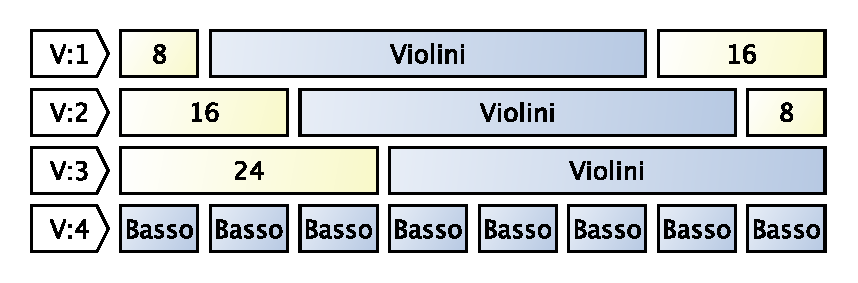
\includegraphics[width=0.8\textwidth]{img/pcanon_scheme.pdf}
    \caption{\canonabc{}'s output scheme}
    \label{fig:pcanon_scheme}
  \end{center}
\end{figure}


\section{Working Together}
This section shows a real example of how to combine three of the \abcpt{}s created: \catabc{},
\pasteabc{} and \learningabc{}.

In this example, a user wants to study his voice (\emph{Tenor}) and \emph{Soprano}'s on the first three sections
of the \emph{Christmas Villancico}\footnote{A Villancico is a musical and poetic form written in
Spanish and Portuguese, traditional from Spain, Latin America and Portugal. These pieces were
popular between century XV and XVIII.} \textit{Verbum caro factum est}.

Each section and voice is written in separate files, so the parts requested will be assembled by
combining \pasteabc{} with \catabc{}.

Then \learningabc{} is going to be used with the combined score in order to produce two scores: one
where voice \emph{Tenor} is highlighted and another where the other voices are.

Listing \ref{lst:cat_paste_by_example} shows the first step being put into action. Listing
\ref{lst:verbum} shows its output, which, in this section, is going to be referred to as
\emph{verbum.abc} and figure \ref{fig:verbum} the corresponding score.\\

\begin{lstlisting}[caption={\catabc{} and \pasteabc{} by example},label={lst:cat_paste_by_example},captionpos=t,abovecaptionskip=-\medskipamount]
cat_abc (
  paste_abc ( 101.abc 103.abc )
  cat_abc   ( 201.abc 303.abc )
) > verbum.abc
\end{lstlisting}

\vspace{1cm}
\lstinputlisting[caption={\emph{verbum.abc}},label={lst:verbum},captionpos=t,abovecaptionskip=-\medskipamount]{misc/verbum.tex}

% \vspace{-1.30cm}
\begin{figure}[H]
  \centering
  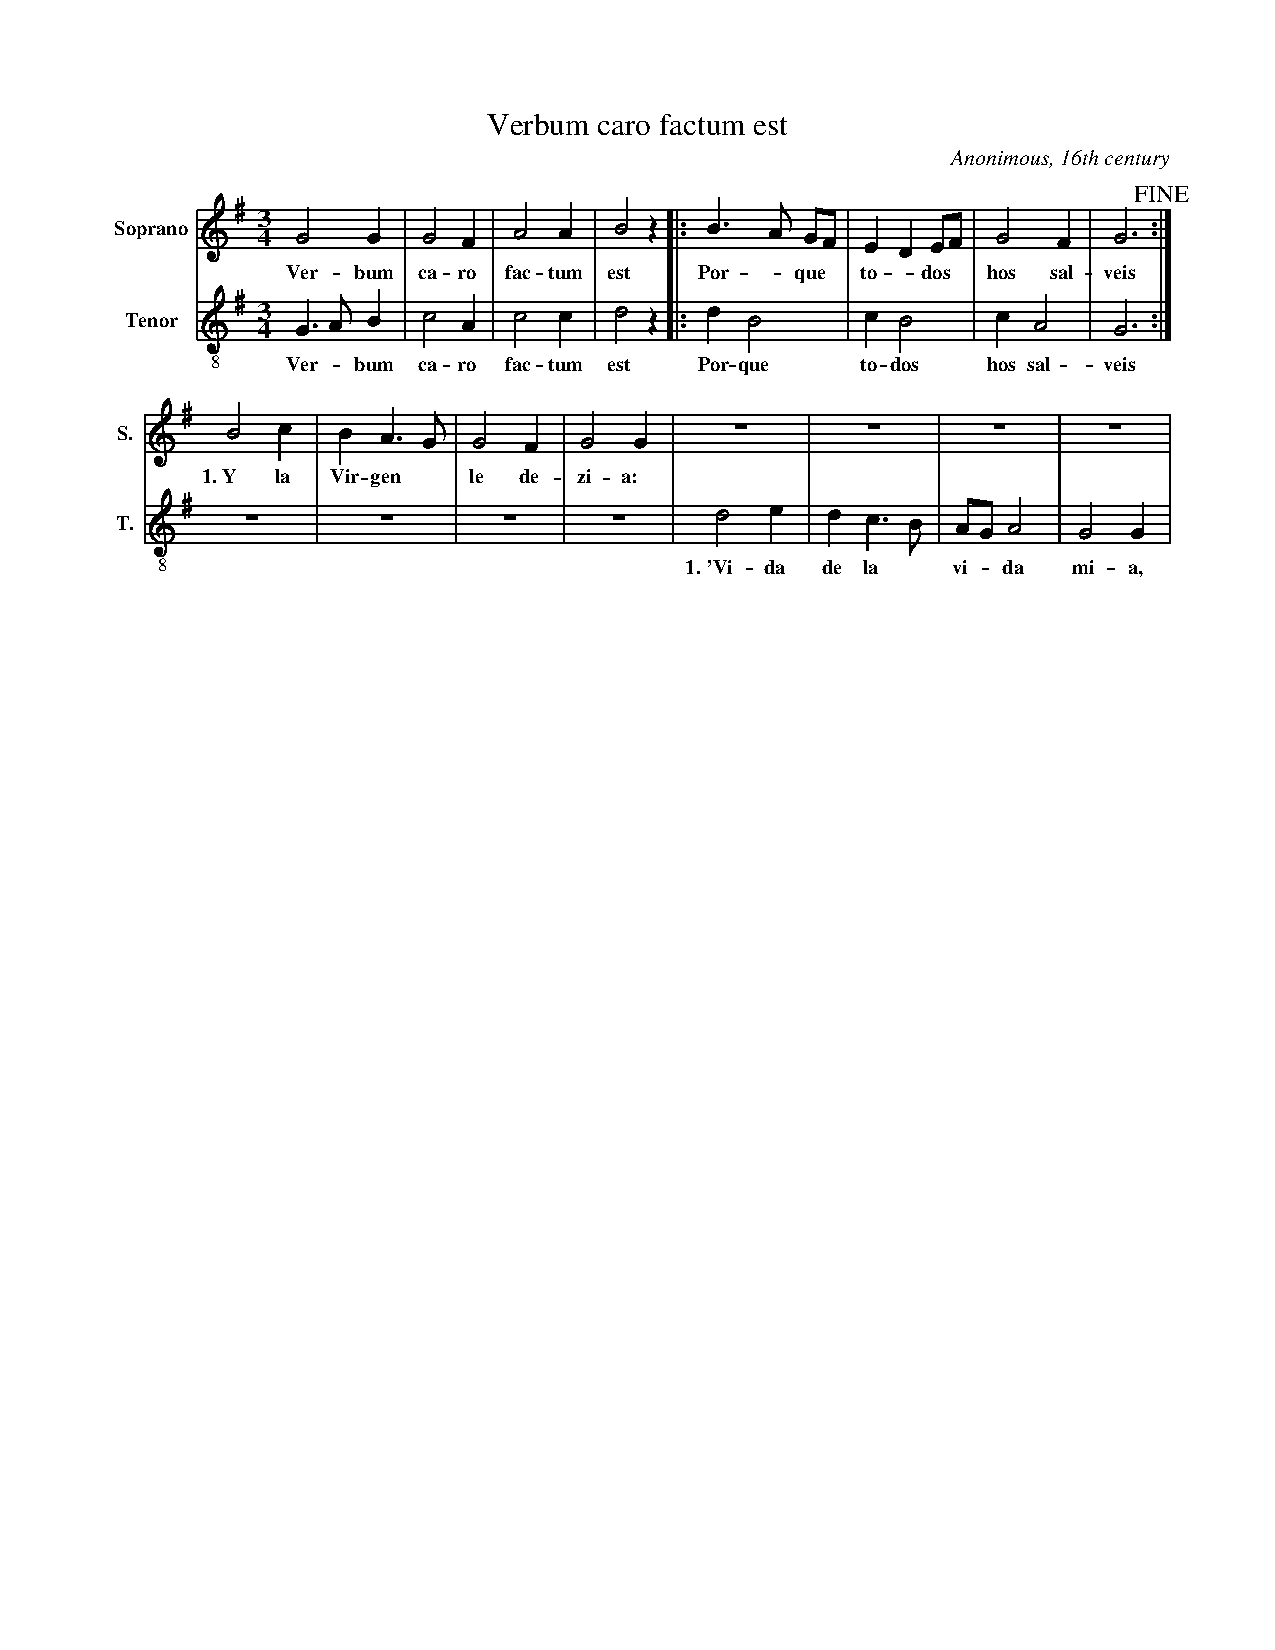
\includegraphics[width=0.8\textwidth, clip=true, trim = 15mm 180mm 15mm 30mm]{img/verbum.pdf}
  \caption{Verbum caro factum est Score: Sections 1, 2 \& 3; Parts 1 \& 3}
  \label{fig:verbum}
\end{figure}

After putting the score together, it's time to modify it in order to help the user study. So
\learningabc{} (see listing \ref{lst:learning_on_cat_paste}) generates a score where just voice
\emph{Tenor} is highlighted (\ref{lst:just_tenor}) and one where all voices but \emph{Tenor}'s are
highlighted (\ref{lst:all_but_tenor}).\\

\begin{lstlisting}[caption={\learningabc{} on combined score},label={lst:learning_on_cat_paste},captionpos=t,abovecaptionskip=-\medskipamount]
learning_abc -v=Tenor verbum.abc
\end{lstlisting}

\lstinputlisting[caption={verbum\_just\_Tenor.abc},label={lst:just_tenor},captionpos=t,abovecaptionskip=-\medskipamount]{misc/v_just_Tenor.tex}
\lstinputlisting[caption={verbum\_all\_but\_Tenor.abc},label={lst:all_but_tenor},captionpos=t,abovecaptionskip=-\medskipamount]{misc/v_all_but_Tenor.tex}



  \chapter{Test and Evaluation}
  \label{chap:test_eval}
  This chapter's goal is to help measure and analyze the behavior of \abcpt{}s created with \abcdt{}
with real world tasks and to support some claims that have been made throughout this dissertation. A
thorough evaluation was not possible mainly because of time limitations, although it's planned to
happen in the near future.

The \abcpt{} being evaluated is \canonabc{} which will process a real world \abc{} score -
\emph{Pachelbel's Canon}, a canon belonging Pachelbel's \emph{Canon and Gigue for 3 violins and
basso continuo}.

The melodic part (here called \textbf{violini.abc}) can be seen in appendix \ref{sec:pcanon_melody}
and the accompaniment (here called \textbf{basso.abc}) in \ref{sec:pcanon_accomp}.

Listing \ref{lst:canonabc_pach} shows how \canonabc{} is called.\\

\begin{lstlisting}[caption={\canonabc{} for Pachelbel's Canon},label={lst:canonabc_pach},captionpos=t,abovecaptionskip=-\medskipamount]
canon_abc violini.abc+8 violini.abc+16 violini.abc+24 basso.abc++
\end{lstlisting}

The output generated is shown in appendix \ref{sec:pcanon}.\\

Using \wcabc{} on the generated canon (see listing \ref{lst:canon_wc}, the pitch counts were removed
since they are not needed for this explanation), there are 4 voices, each with 168 measures. The
individual melody (\textbf{violini.abc}) has 144 measures (see listing \ref{lst:melody_wc}, pitch
counts removed) and considering that the biggest number of \measurerests{} that are inserted to each
melody is 24 (as can be seen on \ref{lst:canonabc_pach} and \ref{fig:pcanon_scheme}), the number of
expected measures per voice in the canon is 168 (144+24), which matches the count produced in
listing \ref{lst:canon_wc}.\\

\lstinputlisting[caption={\wcabc{} on Pachelbel's Canon},label={lst:canon_wc},captionpos=t,abovecaptionskip=-\medskipamount]{misc/canonwc.tex}

\lstinputlisting[caption={\wcabc{} on Pachelbel's Canon Melody},label={lst:melody_wc},captionpos=t,abovecaptionskip=-\medskipamount]{misc/melodywc.tex}

Furthermore, the number of notes in each of the first three voices (melody parts) is the same as in
the original melody as expected considering that the only thing that \canonabc{} inserts into
melodic parts is \measurerests{}.

The accompaniment part (\textbf{basso.abc}) has 8 notes and 8 measures (see listing
\ref{lst:accomp_wc}, pitch counts removed). Since it is repeated until it has the same number of
measures as the melody, the expected result is 168 notes in 168 measures which matches the count
produced in listing \ref{lst:canon_wc}.\\

\lstinputlisting[caption={\wcabc{} on Pachelbel's Canon Accompaniment},label={lst:accomp_wc},captionpos=t,abovecaptionskip=-\medskipamount]{misc/accompwc.tex}

The execution time for this test's case rounds the 2.3 seconds (see table
\ref{tab:execution_times}). It's quite acceptable since it has 4 voices and 168 measures each which
translates into a lot of external calls to \catabc{} and \pasteabc{} in order to gradually build
each individual voice and finally put them all together.

\begin{center}
  \begin{table}[h]
    \begin{tabular}{|p{10cm}|p{4cm}|}
      \hline
      Tool & Execution Time\footnotemark[1]\\
      \hline
      \hline
      \canonabc{} violini.abc+8 ... ... ... > canon.abc & ~2.3 s
      \\
      \hline

      \hline
      \wcabc{} canon.abc & ~0.4 s
      \\
      \hline
    \end{tabular}
    \caption{Execution times}
    \label{tab:execution_times}
  \end{table}
\end{center}

\footnotetext[1]{The times presented were measured in a 5 year old laptop with the following
features: Processor: 2x Intel(R) Core(TM)2 Duo CPU T9400 \@ 2.53GHz; Memory: 3GB; Operating System:
Linux Mint 13 Maya}

The tool itself wasn't very hard to complete. It has around 85 lines of Perl code (not counting
empty lines), excluding \catabc{} and \pasteabc{} and it was quite quick to put together from the
moment the algorithm was designed.

All in all, this test with a real \abc{} score, even though not being an exhaustive one,
demonstrates that generating scores with many measures, notes and with a few minutes of length is
viable. This operation doesn't involve complex calculations, however there are several traversals to
the \abc{} structure as well as a few auxiliary calculations which affect the overall performance.
In the end it produces the expected result proving that an \abcpt{} built using \abcdt{} can deal
with real \abc{} and not with just some controlled testing tunes.


  % So what?
  % What are the possible applications or recommendations?
  % What contribution does it make to knowledge?
  % What next?
  \chapter{Conclusions and Future Work}
  \label{chap:conclusions_future_work}
  % This chapter presents a summary of the work performed in the context of this dissertation,
% establishing some conclusions about some .
%
% Additionally, future work possibilities are discussed, including .

\section{Conclusions}

The \unix{} philosophy and its simple and successful ideas were essential to the conception of this
dissertation:

\begin{itemize}
  \item The concept of simple and compact tools/commands that solve problems of small complexity and
  can be articulated with others was adopted;
  \item The universal type (the text stream) suggested \abc{} as the obvious universal type since it
  is text as well;
  \item The creation of the language \emph{C} to help developing \unix{} inspired the creation of a
  language as well (a \ac{DSL}) called \abcdt{}.
\end{itemize}

So, the natural course of events is to map some of the existing \unix{} tools into \abc{} ones like
\emph{cat}, \emph{paste} and \emph{wc}.\\


The strategy of creating a robust parser for a reflexive language (Perl) is obtained in 3 steps: 1)
searching the best tool that processes what is wanted; 2) isolating its parser; 3) adding a function
that traverses the parser's generated \ac{IR} and serializes it in order to be evaluated.

The \ac{IR} used must be complete enough to enable the application of many different analytic tasks.
However, that fact doesn't invalidate an approach that starts by generating a sequential and
\sourcewise{} structure and then transforming it into something that suits more complex demands.

Reusing \abcmtops{}' parser was very important to help guarantee this work's quality, coverage and
developing time. The generated \ac{IR} is \sourcewise{} which, along with the calculation of the
current \context{} (consult section \ref{sec:abcdt_rules}), allows performing a
representation-agnostic processing.\\


With the \ac{DSL} \abcdt{} there is a considerable simplification of the process of creating an
\abcpt{} considering the following features:

\begin{itemize}
  \item It's not necessary to specify what doesn't need to be transformed (default functions);
  \item A transformation specification is rule-based which facilitates its writing;
  \item There's a set of rich \actuators{} which allows to precisely select a specific point to
  transform.
\end{itemize}

Using a structured processing of \abc{} allows an \abcpt{} to be described in an effective and
compact way.  Processing a complex structure is possible if divided into smaller parts, i.e.,
applying many surgical transformations to its parts (according to its structure) and composing each
individual result into a single result.

A rule based processor (\abcdt{}'s \dt{} function) makes it possible to write very compact and
effective tools. Most of the processing is done by default, i.e. the user only needs to specify what
needs to be transformed. The default function is the identity function, \emph{toabc()}.

Using Perl as the language embedded into \abcdt{} provides a rich environment to allow easy
processing of text. Furthermore, through the use of data structures, like hashes, the user has
bigger expressive power to specify transformations.\\


Currently, there are tools that process \abc{} with specific purposes as well as big software
packages that integrate a lot of features, however there's always the need to process music, this
is, making custom modifications to the original \abc{}, producing some sort of information,
integrating existing tools, etc... That is the main reason for creating an \ac{OS} comprised of
simple tools for generic \abc{} processing which can be composed with each other, as well as a
versatile environment to create new tools through a compact \ac{DSL} embedded in Perl.

\section{Future Work}

As expected, there are many parts of this work that can be improved and extended. In this section,
only a few are going to be described.

\subsection*{Internal Representation}

A \partwise{} \ac{IR} is more suited to melody processing, while a \timewise{} \ac{IR} is more
suited to harmony processing and a \sourcewise{} to a general, robust processing. These
"\emph{views}" of the \ac{IR} provide different spacial perspectives over a score. Each one of them
covers different aspects of music and can even hide those less relevant.

So there will be a mechanism that, during the \ac{IR}'s traversal, recalculates the structure's
orientation when needed in order to provide different notions of the spacial context.

Consequently, a more thorough investigation on data structures and music representations is required
in order to obtain a set of \ac{IR}s capable of answering to very specific tasks in the best way
possible.

\subsection*{Musical Corpora}

Due to time limitations, no work has been done towards this area of research, even though it's one
of the most interesting areas that can bring a lot of useful features.

Building an \abc{} corpus to serve as testing material for the toolkit and also to train systems
that learn from data is still a main goal.

A set of statistical models is planned to be developed over \abc{} corpora in order to produce
features like automatic classification of scores by genre, time period, author, ...

The composition field has been, from the beginning of this dissertation's writing, postponed due to
its complexity. However, it's definitely an area of research worth working in, therefore one of the
features that will be developed is the automatic generation of music. For instance, training a
program to generate a score that follows a certain style, author, or other characteristics
associated, through the use of models, like \emph{Hidden Markov}~\cite{chai2001folk,Lo2010}. Also,
techniques of text mining~\cite{Tan1999} will be used to extract interesting and non-trivial
patterns from text documents.

\subsection*{ABC::DT}

\abcdt{} is far from being complete, it's actually in constant development. Still, some
improvements, extensions, even fixes are to be done in the near future.

The parser used - \abcmtops{}' - has its own bugs that the author has identified but not fixed yet,
as well as bugs that were identified during \abcdt{}'s development. So, whenever possible, any bug
found will be reported to the author in order to help to the parser's and the tools' it is used in -
\abcmtops{} and \tclabc{} - improvement.\\


The set of available \actuators{} will be expanded to accept even more detailed queries.

Another approach to \actuator{} specification will be devised. What's intended is a richer syntax
for identifying \abc{} elements, one that uses path expressions to navigate through an \abc{} tune
and has a set of standard functions to help selecting \abc{} elements. This approach is very similar
to \emph{XPath}'s\cite{XPath:Online}.

More default functions will be added to \abcdt{}'s API.

The identity function - \toabc{} - is not perfect and still needs some improvements.

\subsection*{Toolkit}
\paragraph{}
More \unix{}-like tools will be developed, such as:
\begin{itemize}
  \item \emph{grep\_abc}\\
    Prints melodic lines that match a pattern
  \item \emph{diff\_abc}\\
    Compares scores, for instance, voice by voice
  \item \emph{cut\_abc}, \emph{sed\_abc}, \emph{head\_abc}, \emph{tail\_abc}, \ldots
\end{itemize}

Other tools are planned to be developed:
\begin{itemize}
  \item \emph{transpose\_abc}\\
    Transposes a score up or down by an interval. There are already some tools that perform this
    task, such as \texttt{abc2abc}~\cite{abc2abc:Online} and the Perl script
    \texttt{transpose\_abc.pl}~\cite{transposeabc:Online}.

    It's desired that this feature is available as a polymorphic \abcdt{}'s function, i.e., it may
    be applied to the \emph{note} element, as well to the \emph{key} element and also an
    \emph{accompaniment chord}.
  \item \emph{fugue\_abc}\\
    Similar to \canonabc{}, only that each voice may change the pitch of the original theme. The
    fugue form, is not simple and has more details to its structure, however this tool may serve as
    an initial structure to build one.
\end{itemize}

For the existing tools a few improvements will be done as well:

\begin{description}
  \item[wc\_abc] \hfill
    \begin{itemize}
      \item Add more counts
      \item Provide options to select specific counts from the output
    \end{itemize}
  \item[canon\_abc] \hfill
    \begin{itemize}
      \item Add the option to assign a name to a voice
      \item Add the option to assign a \midi{} instrument to a voice
    \end{itemize}
  \item[find\_chords\_abc] \hfill
    \begin{itemize}
      \item Add more chord formations to find
    \end{itemize}
  \item[detect\_errors\_abc] \hfill
    \begin{itemize}
      \item Add more errors to detect
      \item Error fixing
        \begin{itemize}
          \item Incomplete measures $\Rightarrow$ Add Rests
          \item Overflowing measures $\Rightarrow$ For example, comment the exceeding elements and
          annotate a FIXME
          \item Final bar $\Rightarrow$ Add bar
        \end{itemize}
    \end{itemize}
\end{description}


  \bibliographystyle{plain}

  \cleardoublepage
  \renewcommand\bibname{References}

  \nocite{*}
  \bibliography{references}
  
  \appendix
\thispagestyle{plain}
  \chapter{abcm2ps's parser IR}
  \label{sec:abcm2ps_parser_ir}

This appendix presents an Haskell specification of the serialized structure generated by an
\abcpt{}'s parsing stage.\\

%% ODER: format ==         = "\mathrel{==}"
%% ODER: format /=         = "\neq "
%
%
\makeatletter
\@ifundefined{lhs2tex.lhs2tex.sty.read}%
  {\@namedef{lhs2tex.lhs2tex.sty.read}{}%
   \newcommand\SkipToFmtEnd{}%
   \newcommand\EndFmtInput{}%
   \long\def\SkipToFmtEnd#1\EndFmtInput{}%
  }\SkipToFmtEnd

\newcommand\ReadOnlyOnce[1]{\@ifundefined{#1}{\@namedef{#1}{}}\SkipToFmtEnd}
% \usepackage{amstext}
% \usepackage{amssymb}
% \usepackage{stmaryrd}
\DeclareFontFamily{OT1}{cmtex}{}
\DeclareFontShape{OT1}{cmtex}{m}{n}
  {<5><6><7><8>cmtex8
   <9>cmtex9
   <10><10.95><12><14.4><17.28><20.74><24.88>cmtex10}{}
\DeclareFontShape{OT1}{cmtex}{m}{it}
  {<-> ssub * cmtt/m/it}{}
\newcommand{\texfamily}{\fontfamily{cmtex}\selectfont}
\DeclareFontShape{OT1}{cmtt}{bx}{n}
  {<5><6><7><8>cmtt8
   <9>cmbtt9
   <10><10.95><12><14.4><17.28><20.74><24.88>cmbtt10}{}
\DeclareFontShape{OT1}{cmtex}{bx}{n}
  {<-> ssub * cmtt/bx/n}{}
\newcommand{\tex}[1]{\text{\texfamily#1}}	% NEU

\newcommand{\Sp}{\hskip.33334em\relax}


\newcommand{\Conid}[1]{\mathit{#1}}
\newcommand{\Varid}[1]{\mathit{#1}}
\newcommand{\anonymous}{\kern0.06em \vbox{\hrule\@width.5em}}
\newcommand{\plus}{\mathbin{+\!\!\!+}}
\newcommand{\bind}{\mathbin{>\!\!\!>\mkern-6.7mu=}}
\newcommand{\rbind}{\mathbin{=\mkern-6.7mu<\!\!\!<}}% suggested by Neil Mitchell
\newcommand{\sequ}{\mathbin{>\!\!\!>}}
\renewcommand{\leq}{\leqslant}
\renewcommand{\geq}{\geqslant}
% \usepackage{polytable}

%mathindent has to be defined
\@ifundefined{mathindent}%
  {\newdimen\mathindent\mathindent\leftmargini}%
  {}%

\def\resethooks{%
  \global\let\SaveRestoreHook\empty
  \global\let\ColumnHook\empty}
\newcommand*{\savecolumns}[1][default]%
  {\g@addto@macro\SaveRestoreHook{\savecolumns[#1]}}
\newcommand*{\restorecolumns}[1][default]%
  {\g@addto@macro\SaveRestoreHook{\restorecolumns[#1]}}
\newcommand*{\aligncolumn}[2]%
  {\g@addto@macro\ColumnHook{\column{#1}{#2}}}

\resethooks

\newcommand{\onelinecommentchars}{\quad-{}- }
\newcommand{\commentbeginchars}{\enskip\{-}
\newcommand{\commentendchars}{-\}\enskip}

\newcommand{\visiblecomments}{%
  \let\onelinecomment=\onelinecommentchars
  \let\commentbegin=\commentbeginchars
  \let\commentend=\commentendchars}

\newcommand{\invisiblecomments}{%
  \let\onelinecomment=\empty
  \let\commentbegin=\empty
  \let\commentend=\empty}

\visiblecomments

\newlength{\blanklineskip}
\setlength{\blanklineskip}{0.66084ex}

\newcommand{\hsindent}[1]{\quad}% default is fixed indentation
\let\hspre\empty
\let\hspost\empty
\newcommand{\NB}{\textbf{NB}}
\newcommand{\Todo}[1]{$\langle$\textbf{To do:}~#1$\rangle$}

\EndFmtInput
\makeatother
%
%
%
%
%
%
% This package provides two environments suitable to take the place
% of hscode, called "plainhscode" and "arrayhscode". 
%
% The plain environment surrounds each code block by vertical space,
% and it uses \abovedisplayskip and \belowdisplayskip to get spacing
% similar to formulas. Note that if these dimensions are changed,
% the spacing around displayed math formulas changes as well.
% All code is indented using \leftskip.
%
% Changed 19.08.2004 to reflect changes in colorcode. Should work with
% CodeGroup.sty.
%
\ReadOnlyOnce{polycode.fmt}%
\makeatletter

\newcommand{\hsnewpar}[1]%
  {{\parskip=0pt\parindent=0pt\par\vskip #1\noindent}}

% can be used, for instance, to redefine the code size, by setting the
% command to \small or something alike
\newcommand{\hscodestyle}{}

% The command \sethscode can be used to switch the code formatting
% behaviour by mapping the hscode environment in the subst directive
% to a new LaTeX environment.

\newcommand{\sethscode}[1]%
  {\expandafter\let\expandafter\hscode\csname #1\endcsname
   \expandafter\let\expandafter\endhscode\csname end#1\endcsname}

% "compatibility" mode restores the non-polycode.fmt layout.

\newenvironment{compathscode}%
  {\par\noindent
   \advance\leftskip\mathindent
   \hscodestyle
   \let\\=\@normalcr
   \let\hspre\(\let\hspost\)%
   \pboxed}%
  {\endpboxed\)%
   \par\noindent
   \ignorespacesafterend}

\newcommand{\compaths}{\sethscode{compathscode}}

% "plain" mode is the proposed default.
% It should now work with \centering.
% This required some changes. The old version
% is still available for reference as oldplainhscode.

\newenvironment{plainhscode}%
  {\hsnewpar\abovedisplayskip
   \advance\leftskip\mathindent
   \hscodestyle
   \let\hspre\(\let\hspost\)%
   \pboxed}%
  {\endpboxed%
   \hsnewpar\belowdisplayskip
   \ignorespacesafterend}

\newenvironment{oldplainhscode}%
  {\hsnewpar\abovedisplayskip
   \advance\leftskip\mathindent
   \hscodestyle
   \let\\=\@normalcr
   \(\pboxed}%
  {\endpboxed\)%
   \hsnewpar\belowdisplayskip
   \ignorespacesafterend}

% Here, we make plainhscode the default environment.

\newcommand{\plainhs}{\sethscode{plainhscode}}
\newcommand{\oldplainhs}{\sethscode{oldplainhscode}}
\plainhs

% The arrayhscode is like plain, but makes use of polytable's
% parray environment which disallows page breaks in code blocks.

\newenvironment{arrayhscode}%
  {\hsnewpar\abovedisplayskip
   \advance\leftskip\mathindent
   \hscodestyle
   \let\\=\@normalcr
   \(\parray}%
  {\endparray\)%
   \hsnewpar\belowdisplayskip
   \ignorespacesafterend}

\newcommand{\arrayhs}{\sethscode{arrayhscode}}

% The mathhscode environment also makes use of polytable's parray 
% environment. It is supposed to be used only inside math mode 
% (I used it to typeset the type rules in my thesis).

\newenvironment{mathhscode}%
  {\parray}{\endparray}

\newcommand{\mathhs}{\sethscode{mathhscode}}

% texths is similar to mathhs, but works in text mode.

\newenvironment{texthscode}%
  {\(\parray}{\endparray\)}

\newcommand{\texths}{\sethscode{texthscode}}

% The framed environment places code in a framed box.

\def\codeframewidth{\arrayrulewidth}
% \RequirePackage{calc}

\newenvironment{framedhscode}%
  {\parskip=\abovedisplayskip\par\noindent
   \hscodestyle
   \arrayrulewidth=\codeframewidth
   \tabular{@{}|p{\linewidth-2\arraycolsep-2\arrayrulewidth-2pt}|@{}}%
   \hline\framedhslinecorrect\\{-1.5ex}%
   \let\endoflinesave=\\
   \let\\=\@normalcr
   \(\pboxed}%
  {\endpboxed\)%
   \framedhslinecorrect\endoflinesave{.5ex}\hline
   \endtabular
   \parskip=\belowdisplayskip\par\noindent
   \ignorespacesafterend}

\newcommand{\framedhslinecorrect}[2]%
  {#1[#2]}

\newcommand{\framedhs}{\sethscode{framedhscode}}

% The inlinehscode environment is an experimental environment
% that can be used to typeset displayed code inline.

\newenvironment{inlinehscode}%
  {\(\def\column##1##2{}%
   \let\>\undefined\let\<\undefined\let\\\undefined
   \newcommand\>[1][]{}\newcommand\<[1][]{}\newcommand\\[1][]{}%
   \def\fromto##1##2##3{##3}%
   \def\nextline{}}{\) }%

\newcommand{\inlinehs}{\sethscode{inlinehscode}}

% The joincode environment is a separate environment that
% can be used to surround and thereby connect multiple code
% blocks.

\newenvironment{joincode}%
  {\let\orighscode=\hscode
   \let\origendhscode=\endhscode
   \def\endhscode{\def\hscode{\endgroup\def\@currenvir{hscode}\\}\begingroup}
   %\let\SaveRestoreHook=\empty
   %\let\ColumnHook=\empty
   %\let\resethooks=\empty
   \orighscode\def\hscode{\endgroup\def\@currenvir{hscode}}}%
  {\origendhscode
   \global\let\hscode=\orighscode
   \global\let\endhscode=\origendhscode}%

\makeatother
\EndFmtInput
%

\begin{hscode}\SaveRestoreHook
\column{B}{@{}>{\hspre}l<{\hspost}@{}}%
\column{15}{@{}>{\hspre}l<{\hspost}@{}}%
\column{17}{@{}>{\hspre}l<{\hspost}@{}}%
\column{18}{@{}>{\hspre}l<{\hspost}@{}}%
\column{19}{@{}>{\hspre}l<{\hspost}@{}}%
\column{49}{@{}>{\hspre}l<{\hspost}@{}}%
\column{E}{@{}>{\hspre}l<{\hspost}@{}}%
\>[B]{}\mbox{\onelinecomment  * Type definitions}{}\<[E]%
\\[\blanklineskip]%
\>[B]{}\mathbf{data}\;\Conid{AbcTunes}\mathrel{=}{}\<[18]%
\>[18]{}\Conid{AbcTunes}\;[\mskip1.5mu \Conid{AbcTune}\mskip1.5mu]{}\<[E]%
\\[\blanklineskip]%
\>[B]{}\mbox{\onelinecomment   Tune definition}{}\<[E]%
\\
\>[B]{}\mathbf{data}\;\Conid{AbcTune}\mathrel{=}{}\<[17]%
\>[17]{}\Conid{AbcTune}\;\{\mskip1.5mu {}\<[E]%
\\
\>[17]{}\hsindent{2}{}\<[19]%
\>[19]{}\Varid{abc\char95 vers}\mathbin{::}\Conid{Int},{}\<[E]%
\\
\>[17]{}\hsindent{2}{}\<[19]%
\>[19]{}\Varid{client\char95 data}\mathbin{::}\Varid{string},{}\<[E]%
\\
\>[17]{}\hsindent{2}{}\<[19]%
\>[19]{}\Varid{micro\char95 tb}\mathbin{::}[\mskip1.5mu \Conid{Int}\mskip1.5mu],{}\<[E]%
\\
\>[17]{}\hsindent{2}{}\<[19]%
\>[19]{}\Varid{symbols}\mathbin{::}[\mskip1.5mu \Conid{AbcSym}\mskip1.5mu]{}\<[E]%
\\
\>[17]{}\mskip1.5mu\}{}\<[E]%
\\[\blanklineskip]%
\>[B]{}\mbox{\onelinecomment   Symbol Definition}{}\<[E]%
\\
\>[B]{}\mathbf{data}\;\Conid{AbcSym}\mathrel{=}{}\<[17]%
\>[17]{}\Conid{AbcSym}\;\{\mskip1.5mu {}\<[E]%
\\
\>[17]{}\hsindent{2}{}\<[19]%
\>[19]{}\mathbf{type}\mathbin{::}\Conid{Int},{}\<[E]%
\\
\>[17]{}\hsindent{2}{}\<[19]%
\>[19]{}\Varid{state}\mathbin{::}\Conid{Int},{}\<[E]%
\\
\>[17]{}\hsindent{2}{}\<[19]%
\>[19]{}\Varid{colnum}\mathbin{::}\Conid{Int},{}\<[E]%
\\
\>[17]{}\hsindent{2}{}\<[19]%
\>[19]{}\Varid{flags}\mathbin{::}\Conid{Int},{}\<[E]%
\\
\>[17]{}\hsindent{2}{}\<[19]%
\>[19]{}\Varid{linenum}\mathbin{::}\Conid{Int},{}\<[E]%
\\
\>[17]{}\hsindent{2}{}\<[19]%
\>[19]{}\Varid{text}\mathbin{::}\Conid{String},{}\<[E]%
\\
\>[17]{}\hsindent{2}{}\<[19]%
\>[19]{}\Varid{comment}\mathbin{::}\Conid{String},{}\<[E]%
\\
\>[17]{}\hsindent{2}{}\<[19]%
\>[19]{}\Varid{u}\mathbin{::}\Conid{SymInfo}{}\<[E]%
\\
\>[17]{}\mskip1.5mu\}{}\<[E]%
\\[\blanklineskip]%
\>[B]{}\mbox{\onelinecomment   Tune Information Definition}{}\<[E]%
\\
\>[B]{}\mathbf{data}\;\Conid{SymInfo}{}\<[15]%
\>[15]{}\mathrel{=}\Conid{Key}\;\{\mskip1.5mu {}\<[49]%
\>[49]{}\mbox{\onelinecomment  K: info}{}\<[E]%
\\
\>[15]{}\hsindent{4}{}\<[19]%
\>[19]{}\Varid{sf}\mathbin{::}\Conid{Int},{}\<[E]%
\\
\>[15]{}\hsindent{4}{}\<[19]%
\>[19]{}\Varid{empty}\mathbin{::}\Conid{Int},{}\<[E]%
\\
\>[15]{}\hsindent{4}{}\<[19]%
\>[19]{}\Varid{exp}\mathbin{::}\Conid{Int},{}\<[E]%
\\
\>[15]{}\hsindent{4}{}\<[19]%
\>[19]{}\Varid{mode}\mathbin{::}\Conid{Int},{}\<[E]%
\\
\>[15]{}\hsindent{4}{}\<[19]%
\>[19]{}\Varid{nacc}\mathbin{::}\Conid{Int},{}\<[E]%
\\
\>[15]{}\hsindent{4}{}\<[19]%
\>[19]{}\Varid{octave}\mathbin{::}\Conid{Int},{}\<[E]%
\\
\>[15]{}\hsindent{4}{}\<[19]%
\>[19]{}\Varid{pits}\mathbin{::}[\mskip1.5mu \Conid{Int}\mskip1.5mu],{}\<[E]%
\\
\>[15]{}\hsindent{4}{}\<[19]%
\>[19]{}\Varid{accs}\mathbin{::}[\mskip1.5mu \Conid{Int}\mskip1.5mu]{}\<[E]%
\\
\>[15]{}\hsindent{2}{}\<[17]%
\>[17]{}\mskip1.5mu\}{}\<[E]%
\\
\>[15]{}\mid \Conid{Length}\;\{\mskip1.5mu {}\<[49]%
\>[49]{}\mbox{\onelinecomment  L: info}{}\<[E]%
\\
\>[15]{}\hsindent{4}{}\<[19]%
\>[19]{}\Varid{base\char95 length}\mathbin{::}\Conid{Int}{}\<[E]%
\\
\>[15]{}\hsindent{2}{}\<[17]%
\>[17]{}\mskip1.5mu\}{}\<[E]%
\\
\>[15]{}\mid \Conid{Meter}\;\{\mskip1.5mu {}\<[49]%
\>[49]{}\mbox{\onelinecomment  M: info}{}\<[E]%
\\
\>[15]{}\hsindent{4}{}\<[19]%
\>[19]{}\Varid{wmeasure}\mathbin{::}\Conid{Int},{}\<[E]%
\\
\>[15]{}\hsindent{4}{}\<[19]%
\>[19]{}\Varid{nmeter}\mathbin{::}\Conid{Int},{}\<[E]%
\\
\>[15]{}\hsindent{4}{}\<[19]%
\>[19]{}\Varid{expdur}\mathbin{::}\Conid{Int},{}\<[E]%
\\
\>[15]{}\hsindent{4}{}\<[19]%
\>[19]{}\Varid{meter}\mathbin{::}[\mskip1.5mu \Conid{MeterDef}\mskip1.5mu]{}\<[E]%
\\
\>[15]{}\hsindent{2}{}\<[17]%
\>[17]{}\mskip1.5mu\}{}\<[E]%
\\
\>[15]{}\mid \Conid{Tempo}\;\{\mskip1.5mu {}\<[49]%
\>[49]{}\mbox{\onelinecomment  Q: info}{}\<[E]%
\\
\>[15]{}\hsindent{4}{}\<[19]%
\>[19]{}\Varid{str1}\mathbin{::}\Conid{String},{}\<[E]%
\\
\>[15]{}\hsindent{4}{}\<[19]%
\>[19]{}\Varid{length}\mathbin{::}[\mskip1.5mu \Conid{Int}\mskip1.5mu],{}\<[E]%
\\
\>[15]{}\hsindent{4}{}\<[19]%
\>[19]{}\Varid{value}\mathbin{::}\Conid{String},{}\<[E]%
\\
\>[15]{}\hsindent{4}{}\<[19]%
\>[19]{}\Varid{str2}\mathbin{::}\Conid{String}{}\<[E]%
\\
\>[15]{}\hsindent{2}{}\<[17]%
\>[17]{}\mskip1.5mu\}{}\<[E]%
\\
\>[15]{}\mid \Conid{Voice}\;\{\mskip1.5mu {}\<[49]%
\>[49]{}\mbox{\onelinecomment  V: info}{}\<[E]%
\\
\>[15]{}\hsindent{4}{}\<[19]%
\>[19]{}\Varid{id}\mathbin{::}\Conid{String},{}\<[E]%
\\
\>[15]{}\hsindent{4}{}\<[19]%
\>[19]{}\Varid{fname}\mathbin{::}\Conid{String},{}\<[E]%
\\
\>[15]{}\hsindent{4}{}\<[19]%
\>[19]{}\Varid{nname}\mathbin{::}\Conid{String},{}\<[E]%
\\
\>[15]{}\hsindent{4}{}\<[19]%
\>[19]{}\Varid{scale}\mathbin{::}\Conid{Float},{}\<[E]%
\\
\>[15]{}\hsindent{4}{}\<[19]%
\>[19]{}\Varid{voice}\mathbin{::}\Conid{Int},{}\<[E]%
\\
\>[15]{}\hsindent{4}{}\<[19]%
\>[19]{}\Varid{octave}\mathbin{::}\Conid{Int},{}\<[E]%
\\
\>[15]{}\hsindent{4}{}\<[19]%
\>[19]{}\Varid{merge}\mathbin{::}\Conid{Int},{}\<[E]%
\\
\>[15]{}\hsindent{4}{}\<[19]%
\>[19]{}\Varid{stem}\mathbin{::}\Conid{Int},{}\<[E]%
\\
\>[15]{}\hsindent{4}{}\<[19]%
\>[19]{}\Varid{gstem}\mathbin{::}\Conid{Int},{}\<[E]%
\\
\>[15]{}\hsindent{4}{}\<[19]%
\>[19]{}\Varid{dyn}\mathbin{::}\Conid{Int},{}\<[E]%
\\
\>[15]{}\hsindent{4}{}\<[19]%
\>[19]{}\Varid{lyrics}\mathbin{::}\Conid{Int},{}\<[E]%
\\
\>[15]{}\hsindent{4}{}\<[19]%
\>[19]{}\Varid{gchord}\mathbin{::}\Conid{Int}{}\<[E]%
\\
\>[15]{}\hsindent{2}{}\<[17]%
\>[17]{}\mskip1.5mu\}{}\<[E]%
\\
\>[15]{}\mid \Conid{Bar}\;\{\mskip1.5mu {}\<[49]%
\>[49]{}\mbox{\onelinecomment  bar, mrest (multi-measure rest) or mrep (measure repeat)}{}\<[E]%
\\
\>[15]{}\hsindent{4}{}\<[19]%
\>[19]{}\mathbf{type}\mathbin{::}\Conid{Int},{}\<[E]%
\\
\>[15]{}\hsindent{4}{}\<[19]%
\>[19]{}\Varid{repeat\char95 bar}\mathbin{::}\Conid{Int},{}\<[E]%
\\
\>[15]{}\hsindent{4}{}\<[19]%
\>[19]{}\Varid{len}\mathbin{::}\Conid{Int},{}\<[E]%
\\
\>[15]{}\hsindent{4}{}\<[19]%
\>[19]{}\Varid{dotted}\mathbin{::}\Conid{Int},{}\<[E]%
\\
\>[15]{}\hsindent{4}{}\<[19]%
\>[19]{}\Varid{dc}\mathbin{::}\Conid{Deco}{}\<[E]%
\\
\>[15]{}\hsindent{2}{}\<[17]%
\>[17]{}\mskip1.5mu\}{}\<[E]%
\\
\>[15]{}\mid \Conid{Clef}\;\{\mskip1.5mu {}\<[49]%
\>[49]{}\mbox{\onelinecomment  clef (and staff!)}{}\<[E]%
\\
\>[15]{}\hsindent{4}{}\<[19]%
\>[19]{}\Varid{name}\mathbin{::}\Conid{String},{}\<[E]%
\\
\>[15]{}\hsindent{4}{}\<[19]%
\>[19]{}\Varid{staffscale}\mathbin{::}\Conid{Float},{}\<[E]%
\\
\>[15]{}\hsindent{4}{}\<[19]%
\>[19]{}\Varid{stafflines}\mathbin{::}\Conid{Int},{}\<[E]%
\\
\>[15]{}\hsindent{4}{}\<[19]%
\>[19]{}\mathbf{type}\mathbin{::}\Conid{Int},{}\<[E]%
\\
\>[15]{}\hsindent{4}{}\<[19]%
\>[19]{}\Varid{line}\mathbin{::}\Conid{Int},{}\<[E]%
\\
\>[15]{}\hsindent{4}{}\<[19]%
\>[19]{}\Varid{octave}\mathbin{::}\Conid{Int},{}\<[E]%
\\
\>[15]{}\hsindent{4}{}\<[19]%
\>[19]{}\Varid{transpose}\mathbin{::}\Conid{Int},{}\<[E]%
\\
\>[15]{}\hsindent{4}{}\<[19]%
\>[19]{}\Varid{invis}\mathbin{::}\Conid{Int},{}\<[E]%
\\
\>[15]{}\hsindent{4}{}\<[19]%
\>[19]{}\Varid{check\char95 pitch}\mathbin{::}\Conid{Int}{}\<[E]%
\\
\>[15]{}\hsindent{2}{}\<[17]%
\>[17]{}\mskip1.5mu\}{}\<[E]%
\\
\>[15]{}\mid \Conid{Note}\;\{\mskip1.5mu {}\<[49]%
\>[49]{}\mbox{\onelinecomment  note, rest}{}\<[E]%
\\
\>[15]{}\hsindent{4}{}\<[19]%
\>[19]{}\Varid{note}\mathbin{::}\Conid{NoteDef}{}\<[E]%
\\
\>[15]{}\hsindent{2}{}\<[17]%
\>[17]{}\mskip1.5mu\}{}\<[E]%
\\
\>[15]{}\mid \Conid{User}\;\{\mskip1.5mu {}\<[49]%
\>[49]{}\mbox{\onelinecomment  user defined accent}{}\<[E]%
\\
\>[15]{}\hsindent{4}{}\<[19]%
\>[19]{}\Varid{symbol}\mathbin{::}\Conid{Int},{}\<[E]%
\\
\>[15]{}\hsindent{4}{}\<[19]%
\>[19]{}\Varid{value}\mathbin{::}\Conid{Int}{}\<[E]%
\\
\>[15]{}\hsindent{2}{}\<[17]%
\>[17]{}\mskip1.5mu\}{}\<[E]%
\\
\>[15]{}\mid \Conid{Eoln}\;\{\mskip1.5mu {}\<[49]%
\>[49]{}\mbox{\onelinecomment  end of line}{}\<[E]%
\\
\>[15]{}\hsindent{4}{}\<[19]%
\>[19]{}\mathbf{type}\mathbin{::}\Conid{Int}{}\<[E]%
\\
\>[15]{}\hsindent{2}{}\<[17]%
\>[17]{}\mskip1.5mu\}{}\<[E]%
\\
\>[15]{}\mid \Conid{VOver}\;\{\mskip1.5mu {}\<[49]%
\>[49]{}\mbox{\onelinecomment  voice overlay}{}\<[E]%
\\
\>[15]{}\hsindent{4}{}\<[19]%
\>[19]{}\mathbf{type}\mathbin{::}\Conid{Int},{}\<[E]%
\\
\>[15]{}\hsindent{4}{}\<[19]%
\>[19]{}\Varid{voice}\mathbin{::}\Conid{Int}{}\<[E]%
\\
\>[15]{}\hsindent{2}{}\<[17]%
\>[17]{}\mskip1.5mu\}{}\<[E]%
\\
\>[15]{}\mid \Conid{Tuplet}\;\{\mskip1.5mu {}\<[49]%
\>[49]{}\mbox{\onelinecomment  tuplet (n:t:x}{}\<[E]%
\\
\>[15]{}\hsindent{4}{}\<[19]%
\>[19]{}\Varid{p\char95 plet}\mathbin{::}\Conid{Int},{}\<[E]%
\\
\>[15]{}\hsindent{4}{}\<[19]%
\>[19]{}\Varid{q\char95 plet}\mathbin{::}\Conid{Int},{}\<[E]%
\\
\>[15]{}\hsindent{4}{}\<[19]%
\>[19]{}\Varid{r\char95 plet}\mathbin{::}\Conid{Int}{}\<[E]%
\\
\>[15]{}\hsindent{2}{}\<[17]%
\>[17]{}\mskip1.5mu\}{}\<[E]%
\\[\blanklineskip]%
\>[B]{}\mbox{\onelinecomment   Meter Definition}{}\<[E]%
\\
\>[B]{}\mathbf{data}\;\Conid{MeterDef}\mathrel{=}\Conid{MeterDef}\;\{\mskip1.5mu {}\<[E]%
\\
\>[B]{}\hsindent{19}{}\<[19]%
\>[19]{}\Varid{top}\mathbin{::}\Conid{String},{}\<[E]%
\\
\>[B]{}\hsindent{19}{}\<[19]%
\>[19]{}\Varid{bot}\mathbin{::}\Conid{String}{}\<[E]%
\\
\>[B]{}\hsindent{17}{}\<[17]%
\>[17]{}\mskip1.5mu\}{}\<[E]%
\\[\blanklineskip]%
\>[B]{}\mbox{\onelinecomment   Note Definition}{}\<[E]%
\\
\>[B]{}\mathbf{data}\;\Conid{NoteDef}{}\<[15]%
\>[15]{}\mathrel{=}\Conid{NoteDef}\;\{\mskip1.5mu {}\<[49]%
\>[49]{}\mbox{\onelinecomment  note or rest}{}\<[E]%
\\
\>[15]{}\hsindent{4}{}\<[19]%
\>[19]{}\Varid{pits}\mathbin{::}[\mskip1.5mu \Conid{Int}\mskip1.5mu],{}\<[E]%
\\
\>[15]{}\hsindent{4}{}\<[19]%
\>[19]{}\Varid{lens}\mathbin{::}[\mskip1.5mu \Conid{Int}\mskip1.5mu],{}\<[E]%
\\
\>[15]{}\hsindent{4}{}\<[19]%
\>[19]{}\Varid{accs}\mathbin{::}[\mskip1.5mu \Conid{Int}\mskip1.5mu],{}\<[E]%
\\
\>[15]{}\hsindent{4}{}\<[19]%
\>[19]{}\Varid{sl1}\mathbin{::}[\mskip1.5mu \Conid{Int}\mskip1.5mu],{}\<[E]%
\\
\>[15]{}\hsindent{4}{}\<[19]%
\>[19]{}\Varid{sl2}\mathbin{::}[\mskip1.5mu \Conid{Int}\mskip1.5mu],{}\<[E]%
\\
\>[15]{}\hsindent{4}{}\<[19]%
\>[19]{}\Varid{ti1}\mathbin{::}[\mskip1.5mu \Conid{Int}\mskip1.5mu],{}\<[E]%
\\
\>[15]{}\hsindent{4}{}\<[19]%
\>[19]{}\Varid{decs}\mathbin{::}[\mskip1.5mu \Conid{Int}\mskip1.5mu],{}\<[E]%
\\
\>[15]{}\hsindent{4}{}\<[19]%
\>[19]{}\Varid{chlen}\mathbin{::}\Conid{Int},{}\<[E]%
\\
\>[15]{}\hsindent{4}{}\<[19]%
\>[19]{}\Varid{nhd}\mathbin{::}\Conid{Int},{}\<[E]%
\\
\>[15]{}\hsindent{4}{}\<[19]%
\>[19]{}\Varid{slur\char95 st}\mathbin{::}\Conid{Int},{}\<[E]%
\\
\>[15]{}\hsindent{4}{}\<[19]%
\>[19]{}\Varid{slur\char95 end}\mathbin{::}\Conid{Int},{}\<[E]%
\\
\>[15]{}\hsindent{4}{}\<[19]%
\>[19]{}\Varid{brhythm}\mathbin{::}\Conid{Int},{}\<[E]%
\\
\>[15]{}\hsindent{4}{}\<[19]%
\>[19]{}\Varid{dc}\mathbin{::}\Conid{Deco}{}\<[E]%
\\
\>[15]{}\hsindent{2}{}\<[17]%
\>[17]{}\mskip1.5mu\}{}\<[E]%
\\[\blanklineskip]%
\>[B]{}\mbox{\onelinecomment  Decoration Definition}{}\<[E]%
\\
\>[B]{}\mathbf{data}\;\Conid{Deco}{}\<[15]%
\>[15]{}\mathrel{=}\Conid{Deco}\;\{\mskip1.5mu {}\<[49]%
\>[49]{}\mbox{\onelinecomment  decorations}{}\<[E]%
\\
\>[15]{}\hsindent{4}{}\<[19]%
\>[19]{}\Varid{n}\mathbin{::}\Conid{Int},{}\<[E]%
\\
\>[15]{}\hsindent{4}{}\<[19]%
\>[19]{}\Varid{h}\mathbin{::}\Conid{Int},{}\<[E]%
\\
\>[15]{}\hsindent{4}{}\<[19]%
\>[19]{}\Varid{s}\mathbin{::}\Conid{Int},{}\<[E]%
\\
\>[15]{}\hsindent{4}{}\<[19]%
\>[19]{}\Varid{t}\mathbin{::}[\mskip1.5mu \Conid{Int}\mskip1.5mu]{}\<[E]%
\\
\>[15]{}\hsindent{2}{}\<[17]%
\>[17]{}\mskip1.5mu\}{}\<[E]%
\ColumnHook
\end{hscode}\resethooks


  \chapter{ABC::DT}
  This appendix presents \abcdtrules{}' list of existing actuators and a list of the functions that
\abcdt{} provides.

\section{ABC::DT Rules' Actuators}
\label{sec:abcdt_rules_actuators}

This appendix presents \abcdtrules{}' list of existing actuators.

\begin{center}
  \begin{tabular}{|p{2cm}|p{4.5cm}|p{3.5cm}|p{5cm}|}
    \hline
    Scope & Actuator & Example & Description \\
    \hline
    \hline
    \multirow{4}{*}{GENERAL}
    & <state>
    & 'in\_header'
    & Selects all \abc{} elements that appear in context <state> (in\_global, in\_header, in\_tune, in\_header)
    \\ \cline{2-4}
    \hline

    \hline
    \multirow{3}{*}{SPECIAL}
    & '-default'
    &
    & Default transformation for unselected \abc{} elements
    \\ \cline{2-4}

    & '-end'
    &
    & General post processing
    \\ \cline{2-4}
    \hline

    \hline
    \multirow{8}{*}{PSCOM}
    & 'pscom'
    &
    & Selects all formatting commands; Any element starting with '\%\%'
    \\ \cline{2-4}

    & 'FORMAT'
    &
    & Selects all formatting commands
    \\ \cline{2-4}

    & 'FORMAT::' . <formatting\_command>
    & 'FORMAT::staves'
    & Selects a specific formatting command
    \\ \cline{2-4}

    & 'MIDI'
    &
    & Selects all abcMIDI commands
    \\ \cline{2-4}

    & 'MIDI::' . <abc\_midi>
    & 'MIDI::channel'
    & Selects a specific abcMIDI command
    \\ \cline{2-4}
    \hline

  \end{tabular}
\end{center}

\begin{center}
  \begin{tabular}{|p{1.75cm}|p{4cm}|p{3cm}|p{6cm}|}
    \hline
    Scope & Actuator & Example & Description \\
    \hline
    \hline
    \multirow{15}{*}{NOTE}
    & 'note'
    &
    & Selects all \abc{} elements that are notes
    \\ \cline{2-4}

    & 'note::' . <note>
    & 'note::C'
    & Selects a specific note
    \\ \cline{2-4}

    & 'V:' . <voice\_name> . '::' . 'note'
    & 'V:Tenor::note'
    & Selects a note that appears in the context of a voice with name <voice\_name>
    \\ \cline{2-4}

    & 'V:' . <voice\_id> . '::' . 'note'
    & 'V:2::note'
    & Selects a note that appears in the context of a voice with id <voice\_id>
    \\ \cline{2-4}

    & 'V:' . <voice\_name> . '::' . 'note::' . <note>
    & 'V:Tenor::note::C'
    & Selects a specific note that appears in the context of a voice with name <voice\_name>
    \\ \cline{2-4}

    & 'V:' . <voice\_id> . '::' . 'note::' . <note>
    & 'V:2::note::C'
    & Selects a specific note that appears in the context of a voice with id <voice\_id>
    \\ \cline{2-4}
    \hline

    \hline
    \multirow{8}{*}{REST}
    & 'rest'
    &
    & Selects all \abc{} elements that are rests
    \\ \cline{2-4}

    & 'V:' . <voice\_name> . '::' . 'rest'
    & 'V:Tenor::rest'
    & Selects a rest that appears in the context of a voice with name <voice\_name>
    \\ \cline{2-4}

    & 'V:' . <voice\_id> . '::' . 'rest'
    & 'V:2::rest'
    & Selects a rest that appears in the context of a voice with id <voice\_id>
    \\ \cline{2-4}
    \hline

    \hline
    \multirow{9}{*}{BAR}
    & 'bar'
    &
    & Selects all \abc{} elements that are bars
    \\ \cline{2-4}

    & <bar>
    & ':|'
    & Selects a specific bar
    \\ \cline{2-4}

    & 'V:' . <voice\_name> . '::' . 'bar'
    & 'V:Tenor::bar'
    & Selects a bar that appears in the context of a voice with name <voice\_name>
    \\ \cline{2-4}

    & 'V:' . <voice\_id> . '::' . 'bar'
    & 'V:2::bar'
    & Selects a bar that appears in the context of a voice with id <voice\_id>
    \\ \cline{2-4}
    \hline

  \end{tabular}
\end{center}

\begin{center}
  \begin{tabular}{|p{1.75cm}|p{3.5cm}|p{3cm}|p{7cm}|}
    \hline
    Scope & Actuator & Example & Description \\
    \hline
    \hline
    \multirow{11}{*}{GCHORD}
    & 'gchord'
    &
    & Selects all \abc{} elements that are accompaniment chords
    \\ \cline{2-4}

    & 'gchord::' . <gchord>
    & 'gchord::F'
    & Selects a specific accompaniment chord
    \\ \cline{2-4}

    & <type> . '::gchord'
    & 'note::gchord'
    & Selects an accompaniment chord that is associated with a <type> (note, rest or bar)
    \\ \cline{2-4}

    & <type> . '::gchord' . <gchord>
    & 'note::gchord::F'
    & Selects a specific accompaniment chord that is associated with a <type> (note, rest or bar)
    \\ \cline{2-4}
    \hline

    \hline
    \multirow{9}{*}{DECO}
    & 'deco'
    &
    & Selects all \abc{} elements that are decorations/ornaments
    \\ \cline{2-4}

    & <deco>
    & '!ff!'
    & Selects a specific decoration
    \\ \cline{2-4}

    & <type> . '::deco'
    & 'note::deco'
    & Selects a decoration that is associated with a <type> (note, rest or bar)
    \\ \cline{2-4}

    & <type> . '::' . <deco>
    &  'note::!ff!'
    & Selects a specific decoration that is associated with a <type> (note, rest or bar)
    \\ \cline{2-4}
    \hline

    \hline
    \multirow{5}{*}{CLEF}
    & 'clef'
    &
    & Selects all \abc{} elements that are clefs
    \\ \cline{2-4}

    & <state> . '::clef'
    & 'in\_tune::clef'
    & Selects a clef that appears in context <state> (in\_global, in\_header, in\_tune, in\_header)
    \\ \cline{2-4}
    \hline

  \end{tabular}
\end{center}


\begin{center}
  \begin{tabular}{|p{1.5cm}|p{3.5cm}|p{3.25cm}|p{7cm}|}
    \hline
    Scope & Actuator & Example & Description \\
    \hline
    \hline
    \multirow{23}{*}{INFO}
    & 'info'
    &
    & Selects all \abc{} elements that are info/headers (key, length, meter, voice, ...)
    \\ \cline{2-4}

    & <info>
    & 'K:'
    & Selects a specific info/header (key, length, meter, voice, ...)
    \\ \cline{2-4}

    & <state> . '::info'
    & 'in\_line::info'
    & Selects an info/header (key, length, meter, voice, ...) that appears in context <state>
    (in\_global, in\_header, in\_tune, in\_header)
    \\ \cline{2-4}

    & <state> . '::' . <info> . ':'
    & 'in\_line::K:'
    & Selects a specific info/header (key, length, meter, voice, ...) that appears in context
    <state> (in\_global, in\_header, in\_tune, in\_header)
    \\ \cline{2-4}

    & 'M:' . <meter>
    & 'M:3/4'
    & Selects a meter with text <meter>
    \\ \cline{2-4}

    & <state> . '::M:' . <meter>
    & 'in\_line::M:3/4'
    & Selects a meter with text <meter> that appears in context <state> (in\_global, in\_header, in\_tune, in\_header)
    \\ \cline{2-4}


    & 'V:' . <voice\_name>
    & 'V:Tenor'
    & Selects a voice with name <voice\_name>
    \\ \cline{2-4}

    & 'V:' . <voice\_id>
    & 'V:2'
    & Selects a voice with id <voice\_id>
    \\ \cline{2-4}

    & <state> . '::V:' . <voice\_name>
    & 'in\_line::V:Tenor'
    & Selects a voice with name <voice\_name> that appears in context <state> (in\_global, in\_header, in\_tune, in\_header)
    \\ \cline{2-4}

    & <state> . '::V:' . <voice\_id>
    & 'in\_line::V:2'
    & Selects a voice with id <voice\_id> that appears in context <state> (in\_global, in\_header, in\_tune, in\_header)
    \\ \cline{2-4}
    \hline

    \hline
    \multirow{5}{*}{OTHER}
    & <type>
    & 'tuplet'
    & Selects all \abc{} elements that are <type> (eoln (end of line), mrest (measure rest), mrep (measure
      repeat), v\_over (voice overlay) or tuplet)
    \\ \cline{2-4}
    \hline
  \end{tabular}
\end{center}


\section{ABC::DT Functions}
\label{sec:abcdt_functions}

This appendix presents a list of the functions that \abcdt{} provides.

\begin{center}
  \begin{tabular}{|p{3.5cm}|p{2cm}|p{5.5cm}|p{4cm}|}
    \hline
    Function & Arguments & Description & Notes \\
    \hline
    \hline
    \emph{dt()}
    & \emph{\$abc\_file}, \emph{\%rules}
    & Processes \abc{} tunes. Receives the filename of an \abc{} tune and a set of functions
    (\emph{\%rules}) defining the processing and associated values for each \abc{} element.
    &
    \\
    \hline

    \hline
    \emph{dt\_string()}
    & \emph{\$abc\_string}, \emph{\%rules}
    & Processes \abc{} tunes. Receives an \abc{} tune in string format and a set of functions
    (\emph{\%rules}) defining the processing and associated values for each \abc{} element.
    &
    \\
    \hline

    \hline
    \multirow{5}{*}{\emph{toabc()}}
    & \multirow{5}{*}{\emph{\$sym}}
    & \abcdt{} main processor's default function. The identity function. It produces the original
    \abc{} for a given \ac{IR} element (\abc{} element)
    & Inspired on Jean-François Moine's \tclabc{} \symdumpi{} function.
    \\
    \hline

    \hline
    \multirow{4}{*}{\emph{get\_chords()}}
    & \multirow{4}{*}{\emph{\$sym}}
    & Produces the guitar/accompaniment chords that come associated with a note, rest or bar.
    &
    \\
    \hline

    \hline
    \multirow{2}{*}{\emph{get\_key()}}
    &
    & Returns the current voice's key
    &
    \\
    \hline

    \hline
    \multirow{2}{*}{\emph{get\_length()}}
    &
    & Returns the current voice's note length
    &
    \\
    \hline

    \hline
    \multirow{2}{*}{\emph{get\_meter()}}
    &
    & Returns the current voice's tune meter
    &
    \\
    \hline

  \end{tabular}
\end{center}

\begin{center}
  \begin{tabular}{|p{2.75cm}|p{2.25cm}|p{5.5cm}|p{4.5cm}|}
    \hline
    Function & Arguments & Description & Notes \\
    \hline
    \hline
    \multirow{2}{*}{\emph{get\_wmeasure()}}
    &
    & Returns the current voice's expected measure duration
    &
    \\
    \hline

    \hline
    \multirow{4}{*}{\emph{get\_time()}}
    &
    & Returns the elapsed time (in the internal time representation) until the current element.
    &
    \\
    \hline

    \hline
    \multirow{3}{*}{\emph{get\_time\_ql()}}
    &
    & Returns the elapsed time (in quarter notes) until the current element.
    &
    \\
    \hline

    \hline
    \multirow{4}{*}{\emph{get\_chord\_step()}}
    & \multirow{4}{3cm}{\emph{\$sym}, \emph{\$chord\_step}, \emph{\$test\_root}}
    & Returns the (first) note structure found on the chord (\emph{\$sym}) (\abc{} element
    \emph{note}) at the provided scale degree (\emph{\$chord\_step}). Returns \texttt{undef} if none
    can be found.
    & Inspired in Music21 \texttt{music21.chord} module's \emph{getChordStep()} method.
    \\
    \hline

    \hline
    \multirow{3}{*}{\emph{get\_fifth()}}
    & \multirow{3}{*}{\emph{\$sym}}
    & Returns a note structure describing the fifth of the chord (\emph{\$sym}) (\abc{} element
    \emph{note}).  Shortcut for \emph{get\_chord\_step(5)}.
    & Inspired in Music21 \texttt{music21.chord} module's \emph{getFifth()} method.
    \\
    \hline

    \hline
    \multirow{4}{*}{\emph{get\_third()}}
    & \multirow{4}{*}{\emph{\$sym}}
    & Returns a note structure describing the third of the chord (\emph{\$sym}) (\abc{} element
    \emph{note}).  Shortcut for \emph{get\_chord\_step(3)}.
    & Inspired in Music21 \texttt{music21.chord} module's \emph{getThird()} method.
    \\
    \hline

    \hline
    \multirow{4}{*}{\emph{get\_seventh()}}
    & \multirow{4}{*}{\emph{\$sym}}
    & Returns a note structure describing the seventh of the chord (\emph{\$sym}) (\abc{} element
    \emph{note}).  Shortcut for \emph{get\_chord\_step(7)}.
    & Inspired in Music21 \texttt{music21.chord} module's \emph{getSeventh()} method.
    \\
    \hline

  \end{tabular}
\end{center}

\begin{center}
  \begin{tabular}{|p{2.75cm}|p{2cm}|p{5.75cm}|p{4.5cm}|}
    \hline
    Function & Arguments & Description & Notes \\
    \hline
    \hline
    \multirow{12}{*}{\emph{is\_major\_triad()}}
    & \multirow{12}{*}{\emph{\$sym}}
    & Returns True if the chord (\emph{\$sym}) (\abc{} element \emph{note}) is a Major Triad, that
    is, if it contains only notes that are either in unison with the root, a major third above the
    root, or a perfect fifth above the root. Additionally, it must contain at least one of each
    third and fifth above the root. The chord must be spelled correctly. Otherwise returns False.
    & Inspired in Music21 \texttt{music21.chord} module's \emph{isMajorTriad()} method.
    \\
    \hline

    \hline
    \multirow{12}{*}{\emph{is\_minor\_triad()}}
    & \multirow{12}{*}{\emph{\$sym}}
    & Returns True if the chord (\emph{\$sym}) (\abc{} element \emph{note}) is a Minor Triad, that
    is, if it contains only notes that are either in unison with the root, a minor third above the
    root, or a perfect fifth above the root. Additionally, it must contain at least one of each
    third and fifth above the root. The chord must be spelled correctly. Otherwise returns False.
    & Inspired in Music21 \texttt{music21.chord} module's \emph{isMinor()} method.
    \\
    \hline

    \hline
    \multirow{9}{3cm}{\emph{is\_dominant\_ seventh()}}
    & \multirow{9}{*}{\emph{\$sym}}
    & Returns True if the chord (\emph{\$sym}) (\abc{} element \emph{note}) is a Dominant Seventh,
    that is, if it contains only notes that are either in unison with the root, a major third above
    the root, a perfect fifth, or a major seventh above the root. Additionally, must contain at
    least one of each third and fifth above the root. Chord must be spelled correctly. Otherwise
    returns false.
    & Inspired in Music21 \texttt{music21.chord} module's \emph{isDominantSeventh()} method.
    \\
    \hline

  \end{tabular}
\end{center}

\begin{center}
  \begin{tabular}{|p{3.25cm}|p{2cm}|p{5.25cm}|p{4.5cm}|}
    \hline
    Function & Arguments & Description & Notes \\
    \hline
    \hline
    \multirow{5}{3cm}{\emph{find\_consecutive\_
    notes\_in\_measure()}}
    & \multirow{5}{*}{\emph{\$args}}
    & Returns a list of consecutive note structures belonging to the same measure. Receives an hash
    of options to filter the search (\emph{\$args}).
    & Inspired in Music21 \texttt{music21.stream} module's \emph{findConsecutiveNotes()} method.
    \\
    \hline

    \hline
    \multirow{3}{*}{\emph{root()}}
    & \multirow{3}{*}{\emph{\$sym}}
    & Looks for the chord's (\emph{\$sym}) root by finding the note with the most 3rds above it.
    & Inspired in Music21 \texttt{music21.chord} module's \emph{root()} method.
    \\
    \hline

    \hline
    \multirow{4}{*}{\emph{get\_pitch\_class()}}
    & \multirow{4}{*}{\emph{\$note}}
    & Returns the pitch class of the note. The pitch\_class is a number from 0-11, where 0 = C, 1 =
    C\#/D-, etc.
    & Inspired in Music21 \texttt{music21.pitch} module's \emph{pitchClass} attribute.
    \\
    \hline

    \hline
    \multirow{2}{*}{\emph{get\_pitch\_name()}}
    & \multirow{2}{*}{\emph{\$note}}
    & Returns the pitch name of a note: A-flat, C-sharp.
    & Inspired in Music21 \texttt{music21.pitch} module.
    \\
    \hline
  \end{tabular}
\end{center}


  \chapter{Pachelbel's Canon}
  X:1
T:Canon per Violini e Basso
C:Johann Pachelbel
C:(1653-1706)
M:C
L:1/4
K:D
V:1
Z8|
f4| e4| d4| c4| B4| A4| B4| c4|
d4| c4| B4| A4| G4| F4| G4| E4|
D2F2| A2G2| F2D2| F2E2| D2B,2| D2A2| G2B2| A2G2|
F2D2| E2c2| d2f2| a2A2| B2G2| A2F2| D2d2| Td3c|
dcdD| CAEF| DdcB| cfab| gfeg| fedc| BAGF| EGFE|
DEFG| AEAG| FBAG| AGFE| DB,Bc| dcBA| GFEB| ABAG|
F2f2| e4| z2d2| f4| b4| a4| b4| c'4|
d'2d2| c4| z2B2| d4| d4-|d2d2| d2g2| e2a2|
af/g/ af/g/| a/A/B/c/ d/e/f/g/| fd/e/ fF/G/| A/B/A/G/ A/F/G/A/| GB/A/ GF/E/| F/E/D/E/ F/G/A/B/| GB/A/ Bc/d/| A/B/c/d/ e/f/g/a/|
fd/e/ fe/d/| e/c/d/e/ f/e/d/c/| dB/c/ dD/E/| F/G/F/E/ F/d/c/d/|Bd/c/ BA/G/| A/G/F/G/ A/B/c/d/| Bd/c/ dc/B/| c/d/e/d/ c/d/B/c/|
d2d2|c4|z2B2|d4|D4|D2D2|D2G2|A2E2|
F2f2| e4| z2d2| A4| B4| A4| B4| c4|
dcdD| CAEF| DdcB| cfab| gfeg| fedc| BAGF| EGFE|
DEFG| AEAG| FBAG| AGFE| DB,Bc| dcBA| GFEB| ABAG|
F2D2| E2c2| d2f2| a2A2| B2G2| A2F2| D2d2| c2E2|
D2F2| A2G2| F2D2| F2E2| D2B,2| D2A2| G2B2| A2c2|
d4| c4| B4| A4| G4| F4| G4| A4|
f4| e4| d4| c4| B4| A4| B4| c4|
V:2
Z16|
f4| e4| d4| c4| B4| A4| B4| c4|
d4| c4| B4| A4| G4| F4| G4| E4|
D2F2| A2G2| F2D2| F2E2| D2B,2| D2A2| G2B2| A2G2|
F2D2| E2c2| d2f2| a2A2| B2G2| A2F2| D2d2| Td3c|
dcdD| CAEF| DdcB| cfab| gfeg| fedc| BAGF| EGFE|
DEFG| AEAG| FBAG| AGFE| DB,Bc| dcBA| GFEB| ABAG|
F2f2| e4| z2d2| f4| b4| a4| b4| c'4|
d'2d2| c4| z2B2| d4| d4-|d2d2| d2g2| e2a2|
af/g/ af/g/| a/A/B/c/ d/e/f/g/| fd/e/ fF/G/| A/B/A/G/ A/F/G/A/| GB/A/ GF/E/| F/E/D/E/ F/G/A/B/| GB/A/ Bc/d/| A/B/c/d/ e/f/g/a/|
fd/e/ fe/d/| e/c/d/e/ f/e/d/c/| dB/c/ dD/E/| F/G/F/E/ F/d/c/d/|Bd/c/ BA/G/| A/G/F/G/ A/B/c/d/| Bd/c/ dc/B/| c/d/e/d/ c/d/B/c/|
d2d2|c4|z2B2|d4|D4|D2D2|D2G2|A2E2|
F2f2| e4| z2d2| A4| B4| A4| B4| c4|
dcdD| CAEF| DdcB| cfab| gfeg| fedc| BAGF| EGFE|
DEFG| AEAG| FBAG| AGFE| DB,Bc| dcBA| GFEB| ABAG|
F2D2| E2c2| d2f2| a2A2| B2G2| A2F2| D2d2| c2E2|
D2F2| A2G2| F2D2| F2E2| D2B,2| D2A2| G2B2| A2c2|
d4| c4| B4| A4| G4| F4| G4| A4|
f4| e4| d4| c4| B4| A4| B4| c4|
V:3
Z24|
f4| e4| d4| c4| B4| A4| B4| c4|
d4| c4| B4| A4| G4| F4| G4| E4|
D2F2| A2G2| F2D2| F2E2| D2B,2| D2A2| G2B2| A2G2|
F2D2| E2c2| d2f2| a2A2| B2G2| A2F2| D2d2| Td3c|
dcdD| CAEF| DdcB| cfab| gfeg| fedc| BAGF| EGFE|
DEFG| AEAG| FBAG| AGFE| DB,Bc| dcBA| GFEB| ABAG|
F2f2| e4| z2d2| f4| b4| a4| b4| c'4|
d'2d2| c4| z2B2| d4| d4-|d2d2| d2g2| e2a2|
af/g/ af/g/| a/A/B/c/ d/e/f/g/| fd/e/ fF/G/| A/B/A/G/ A/F/G/A/| GB/A/ GF/E/| F/E/D/E/ F/G/A/B/| GB/A/ Bc/d/| A/B/c/d/ e/f/g/a/|
fd/e/ fe/d/| e/c/d/e/ f/e/d/c/| dB/c/ dD/E/| F/G/F/E/ F/d/c/d/|Bd/c/ BA/G/| A/G/F/G/ A/B/c/d/| Bd/c/ dc/B/| c/d/e/d/ c/d/B/c/|
d2d2|c4|z2B2|d4|D4|D2D2|D2G2|A2E2|
F2f2| e4| z2d2| A4| B4| A4| B4| c4|
dcdD| CAEF| DdcB| cfab| gfeg| fedc| BAGF| EGFE|
DEFG| AEAG| FBAG| AGFE| DB,Bc| dcBA| GFEB| ABAG|
F2D2| E2c2| d2f2| a2A2| B2G2| A2F2| D2d2| c2E2|
D2F2| A2G2| F2D2| F2E2| D2B,2| D2A2| G2B2| A2c2|
d4| c4| B4| A4| G4| F4| G4| A4|
f4| e4| d4| c4| B4| A4| B4| c4|
V:2
Z8| 
V:1
Z16| 
V:4
D,4|A,,4| B,,4| F,,4| G,,4| D,,4| G,,4| A,,4|
D,4|A,,4| B,,4| F,,4| G,,4| D,,4| G,,4| A,,4|
D,4|A,,4| B,,4| F,,4| G,,4| D,,4| G,,4| A,,4|
D,4|A,,4| B,,4| F,,4| G,,4| D,,4| G,,4| A,,4|
D,4|A,,4| B,,4| F,,4| G,,4| D,,4| G,,4| A,,4|
D,4|A,,4| B,,4| F,,4| G,,4| D,,4| G,,4| A,,4|
D,4|A,,4| B,,4| F,,4| G,,4| D,,4| G,,4| A,,4|
D,4|A,,4| B,,4| F,,4| G,,4| D,,4| G,,4| A,,4|
D,4|A,,4| B,,4| F,,4| G,,4| D,,4| G,,4| A,,4|
D,4|A,,4| B,,4| F,,4| G,,4| D,,4| G,,4| A,,4|
D,4|A,,4| B,,4| F,,4| G,,4| D,,4| G,,4| A,,4|
D,4|A,,4| B,,4| F,,4| G,,4| D,,4| G,,4| A,,4|
D,4|A,,4| B,,4| F,,4| G,,4| D,,4| G,,4| A,,4|
D,4|A,,4| B,,4| F,,4| G,,4| D,,4| G,,4| A,,4|
D,4|A,,4| B,,4| F,,4| G,,4| D,,4| G,,4| A,,4|
D,4|A,,4| B,,4| F,,4| G,,4| D,,4| G,,4| A,,4|
D,4|A,,4| B,,4| F,,4| G,,4| D,,4| G,,4| A,,4|
D,4|A,,4| B,,4| F,,4| G,,4| D,,4| G,,4| A,,4|
D,4|A,,4| B,,4| F,,4| G,,4| D,,4| G,,4| A,,4|
D,4|A,,4| B,,4| F,,4| G,,4| D,,4| G,,4| A,,4|
D,4|A,,4| B,,4| F,,4| G,,4| D,,4| G,,4| A,,4|


\end{document}
